\documentclass[sigplan,10pt,review,anonymous]{acmart}\settopmatter{printfolios=true,printccs=false,printacmref=false}

\usepackage{float}
%\usepackage{amssymb}
\usepackage{amsmath,amsfonts}
\usepackage[ruled, vlined]{algorithm2e}
\usepackage{graphicx}
\usepackage{textcomp}
\usepackage{xcolor}
\usepackage{listings}
\usepackage{caption}
\usepackage{subcaption}
\usepackage{multirow}
\usepackage{booktabs}
\usepackage{makecell}
\usepackage{galois}
\usepackage{mathpartir}
\usepackage{bussproofs}
\usepackage{mathtools}
\usepackage{colortbl}
\usepackage{hhline}

\EnableBpAbbreviations

\setcopyright{acmcopyright}
\copyrightyear{2018}
\acmYear{2018}
\acmDOI{10.1145/1122445.1122456}
\acmConference[Woodstock '18]{Woodstock '18: ACM Symposium on Neural
  Gaze Detection}{June 03--05, 2018}{Woodstock, NY}
\acmPrice{15.00}
\acmISBN{978-1-4503-XXXX-X/18/06}

% thicker vertical line
\newcolumntype{?}{!{\vrule width 1pt}}

% Styles
\definecolor{dkgreen}{rgb}{0,0.6,0}
\definecolor{gray}{rgb}{0.5,0.5,0.5}
\definecolor{mauve}{rgb}{0.58,0,0.82}
\lstdefinelanguage{JavaScript}{
  keywords={async, await, break, case, catch, class, const, continue, debugger,
    default, delete, do, else, enum, export, extends, false, finally, for,
    function, if, import, in, instanceof, new, null, return, super, switch, this,
    throw, true, try, typeof, var, void, while, with, yield},
  keywordstyle=\color{blue}\bfseries,
  ndkeywordstyle=\color{darkgray}\bfseries,
  identifierstyle=\color{black},
  sensitive=false,
  comment=[l]{//},
  morecomment=[s]{/*}{*/},
  commentstyle=\color{dkgreen}\ttfamily,
  stringstyle=\color{purple}\ttfamily,
  morestring=[b]',
  morestring=[b]"
}
\lstdefinestyle{myJSstyle}{
  language=JavaScript,
  numbers=left,
  stepnumber=1,
  extendedchars=true,
  basicstyle=\footnotesize\ttfamily,
  showstringspaces=false,
  showspaces=false,
  tabsize=2,
  breaklines=true,
  showtabs=false,
  captionpos=b
}

% Basic
\DeclareMathAlphabet{\mathpzc}{T1}{pzc}{m}{it}
\newcommand{\powerset}[1]{\mathcal{P}(#1)}
\newcommand{\imbox}[1]{\mbox{\small \textit{#1}}}
\newcommand{\name}[1]{\textsf{#1}}
\newcommand{\inred}[1]{{\color{red}{#1}}}
\newcommand{\todo}{\inred{TODO}}
\newcommand{\abs}[1]{{#1}^{\#}}
\newcommand{\finmap}{{\xrightarrow[]{\text{fin}}}}
\newcommand{\mapstos}{\;\dot{\mapsto}\;}
\newcommand{\Dom}{\name{Dom}}

% Tool
\newcommand{\tool}{\text{SAFE}_\name{DS}}

% Keywords
\newcommand{\jscode}[1]{\text{\lstinline[style=myJSstyle,numbers=none]!#1!}}
\newcommand{\code}[1]{\texttt{#1}}
\newcommand{\kwif}{\code{if}}
\newcommand{\kwelse}{\code{else}}
\newcommand{\kwret}{\code{ret}}
\newcommand{\kwobj}{\code{\{\}}}
\newcommand{\kwtrue}{\code{true}}
\newcommand{\kwfalse}{\code{false}}

% Notations
\newcommand{\prog}{P}
\newcommand{\labset}{\mathcal{L}}
\newcommand{\lab}{\mathpzc{l}}
\newcommand{\labdot}[1]{{{\bullet_{\lab_{#1}}}}}
\newcommand{\ilab}{\lab_\iota}
\newcommand{\labnext}{\name{next}}
\newcommand{\op}{\name{op}}
\newcommand{\ops}{\dot{\name{op}}}
\newcommand{\inst}{i}
\newcommand{\expr}{e}
\newcommand{\refer}{r}

% Numbers
\newcommand{\numset}{\mathbb{N}}

% States
\newcommand{\stset}{\mathbb{S}}
\newcommand{\st}{\sigma}
\newcommand{\istset}{\stset_\iota}
\newcommand{\ist}{\st_\iota}

% Memories
\newcommand{\memset}{\mathcal{M}}
\newcommand{\absmemset}{\abs{\memset}}
\newcommand{\mem}{M}
\newcommand{\absmem}{\abs{\mem}}

% Contexts
\newcommand{\ctxtset}{\mathbb{C}}
\newcommand{\absctxtset}{\abs{\ctxtset}}
\newcommand{\ctxt}{c}
\newcommand{\absctxt}{\abs{\ctxt}}
\newcommand{\eabsctxt}{\absctxt_\name{env}}

% Transition Relations
\newcommand{\trans}{\leadsto}
\newcommand{\rutrans}{%
            \mathrel{\raisebox{.1em}{%
            \rotatebox[origin=c]{30}{$\trans$}}}}
\newcommand{\rdtrans}{%
            \mathrel{\raisebox{.1em}{%
            \rotatebox[origin=c]{-30}{$\trans$}}}}


% Complete Lattice
\newcommand{\join}{\sqcup}
\newcommand{\meet}{\sqcap}
\newcommand{\bigjoin}{\bigsqcup}
\newcommand{\bigmeet}{\bigsqcap}
\newcommand{\order}{\sqsubseteq}

% Concrete Domains
\newcommand{\dom}{\mathbb{D}}
\newcommand{\elem}{d}
\newcommand{\ielem}{\elem_\iota}

% Abstract Domains
\newcommand{\absdom}{\abs{\dom}}
\newcommand{\abselem}{\abs{\elem}}
\newcommand{\iabselem}{\abs{\elem}_\iota}

% Concrete Semantics
\newcommand{\sem}[1]{[\![{#1}]\!]}
\newcommand{\transfer}{F}
\newcommand{\step}{\name{step}}

% Abstract Semantics
\newcommand{\abssem}[1]{\abs{\sem{#1}}}
\newcommand{\abstransfer}{\abs{\transfer}}
\newcommand{\absstep}{\abs{\step}}

% Abstract Sensitivity
\newcommand{\viewmap}{\delta}
\newcommand{\sabsdom}{\absdom_\viewmap}
\newcommand{\sabselem}{{\abselem_\viewmap}}
\newcommand{\viewset}{\Pi}
\newcommand{\view}{\pi}
\newcommand{\sabsstep}{\absstep_\viewmap}
\newcommand{\viewtrans}[2]{\abssem{#1 \rightarrow #2}}

% Flow Sensitivity
\newcommand{\fs}{\name{FS}}
\newcommand{\fsviewmap}{\viewmap^\fs}

% Locations
\newcommand{\locset}{\mathbb{L}}
\newcommand{\loc}{l}
\newcommand{\abslocset}{\abs\locset}
\newcommand{\absloc}{\abs\loc}

% Variables
\newcommand{\varset}{\mathbb{X}}
\newcommand{\varx}{\code{x}}

% Values
\newcommand{\valset}{\mathbb{V}}
\newcommand{\val}{v}
\newcommand{\pvalset}{\valset_\name{p}}
\newcommand{\pval}{\val_\name{p}}
\newcommand{\fvalset}{\mathbb{F}}
\newcommand{\fval}[2]{\lambda #1. #2}
\newcommand{\strset}{\valset_\name{str}}
\newcommand{\str}{\val_\name{str}}
\newcommand{\absvalset}{\abs{\valset}}
\newcommand{\absval}{\abs{\val}}

\newcommand{\valgamma}{\gamma_\val}

% Addresses
\newcommand{\addrset}{\mathbb{A}}
\newcommand{\eaddrset}{\addrset_\name{env}}
\newcommand{\oaddrset}{\addrset_\name{obj}}
\newcommand{\addr}{a}
\newcommand{\tladdr}{\addr_{\name{top}}}
\newcommand{\absaddrset}{\abs{\addrset}}
\newcommand{\absaddr}{\abs{\addr}}
\newcommand{\eabsaddr}{\absaddr_\name{env}}
\newcommand{\rabsaddr}{\absaddr_\name{ret}}
\newcommand{\oabsaddr}{\absaddr_\name{obj}}

% Abstract Counting
\newcommand{\abscount}{\abs{n}}
\newcommand{\inc}{\name{inc}}
\newcommand{\abscountset}{\abs{\mathbb{N}}}
\newcommand{\abszero}{\abs{0}}
\newcommand{\absone}{\abs{1}}
\newcommand{\absmany}{\abs{\geq\!\!2}}

% Sealed Symbolic Interpretation
\newcommand{\symb}{\omega}
\newcommand{\symbset}{\Omega}
\newcommand{\symbolic}[1]{{#1}_\symb}
\newcommand{\symbstset}{\symbolic{\stset}}
\newcommand{\symbst}{\symbolic{\st}}
\newcommand{\nsymbst}[1]{\st_{\symb,#1}}
\newcommand{\symbmemset}{\symbolic{\memset}}
\newcommand{\symbtrans}{\symbolic{\trans}}
\newcommand{\excst}{\bot}
\newcommand{\symbevt}{\symb_\jscode{evt}}
\newcommand{\symbint}{\symb_\jscode{int}}

% Combined Analysis
\newcommand{\comb}[1]{\widetilde{#1}}
\newcommand{\combdom}{\comb{\dom}}
\newcommand{\combelem}{\comb{\elem}}
\newcommand{\combgamma}{\comb{\gamma}}
\newcommand{\combstep}{\comb{\step}}
\newcommand{\combtransfer}{\comb{\transfer}}
\newcommand{\sgamma}{\gamma_\viewmap}
\newcommand{\converter}{\tau}
\newcommand{\saconverter}{\abs{\converter}}
\newcommand{\asconverter}{\symbolic{\converter}}
\newcommand{\combviewtrans}[2]{\sem{\comb{#1 \rightarrow #2}}}

\newcommand{\symbdom}{\symbolic{\dom}}
\newcommand{\symbelem}{\symbolic{\elem}}
\newcommand{\symbgamma}{\symbolic{\gamma}}
\newcommand{\symbstep}{\symbolic{\step}}

% Legacy
\newcommand{\scombstep}{\comb{\step}_\viewmap}
\newcommand{\scombgamma}{\combgamma_\viewmap}
\newcommand{\scombelem}{\comb{\elem}_\viewmap}

% Triage
\newcommand{\triage}{\name{triage}}
\newcommand{\atriage}{\triage_\aelem}

% Rules
\newcommand{\referrule}[3]{#1 \vdash_\refer #2 \Rightarrow  #3}
\newcommand{\exprrule}[3]{#1 \vdash_\expr #2 \Rightarrow #3}

% Abstract Semantics
\newcommand{\referabssem}[1]{\abssem{#1}_\refer}
\newcommand{\exprabssem}[1]{\abssem{#1}_\expr}

% Identity function
\newcommand{\identity}{\name{id}}

% Checker
\newcommand{\checker}{\name{checker}}

% Concerto
\newcommand{\concerto}{\textsc{Concerto}}

% Table 1
\newcommand{\myhead}[3]{
  \multicolumn{1}{c|}{\textbf{#1}} &
  \multicolumn{1}{c|@{~}}{\textbf{#2}} &
  \multicolumn{4}{@{~}c@{~}?}{\textbf{#3}} &
  \multicolumn{1}{c|}{\textbf{#1}} &
  \multicolumn{1}{c|@{~}}{\textbf{#2}} &
  \multicolumn{4}{@{~}c@{~}?}{\textbf{#3}} &
  \multicolumn{1}{c|}{\textbf{#1}} &
  \multicolumn{1}{c|@{~}}{\textbf{#2}} &
  \multicolumn{4}{@{~}c@{~}}{\textbf{#3}}\\\hline
}
\newcommand{\mydata}[6]{
  \multirow{#1}{*}{\jscode{#2}} &
  \jscode{#3} &
  \text{#4} &
  \text{/} &
  \text{#5} &
  \text{(#6\%)}
}
\newcommand{\mysucccolor}{yellow}
\newcommand{\mysucc}[6]{
  \multirow{#1}{*}{\jscode{#2}} &
  \multicolumn{1}{>{\columncolor{\mysucccolor}}l|@{~}}    {\jscode{#3}} &
  {\text{#4}} &
  {\text{/}} &
  {\text{#5}} &
  {\text{(#6\%)}}
}
\newcommand{\mymult}[6]{
  \jscode{#2} &
  \multirow{#1}{*}{\jscode{#3}} &
  \multirow{#1}{*}{\text{#4}} &
  \multirow{#1}{*}{\text{/}} &
  \multirow{#1}{*}{\text{#5}} &
  \multirow{#1}{*}{\text{(#6\%)}}
}
\newcommand{\myname}[2]{\multirow{#1}{*}{\jscode{#2}}&&&&&}
\newcommand{\mynewline}[6]{
  \\
  \cline{#1-#2}
  \cline{#3-#4}
  \cline{#5-#6}
}
\newcommand{\mylinef}  {\\\hhline{~|-----}}
\newcommand{\mylineff} {\\\hhline{~|-----~|-----}}
\newcommand{\mylinetf} {\\\hhline{------~|-----}}
\newcommand{\mylinefff}{\\\hhline{~|-----~|-----~|-----}}
\newcommand{\mylinefft}{\\\hhline{~|-----~|-----------}}
\newcommand{\mylineftf}{\\\hhline{~|-----------~|-----}}
\newcommand{\mylineftt}{\\\hhline{~|-----------------}}
\newcommand{\mylinetff}{\\\hhline{------~|-----~|-----}}
\newcommand{\mylinetft}{\\\hhline{------~|-----------}}
\newcommand{\mylinettf}{\\\hhline{------------~|-----}}
\newcommand{\mylinettt}{\\\hhline{------------------}}

% Instantiation Map
\newcommand{\imap}{m}
\newcommand{\imapset}{\mathbb{M}}
\newcommand{\absimap}{\abs{\imap}}
\newcommand{\absimapset}{\abs{\imapset}}
\newcommand{\instant}[2]{#1\!\!\mid\!\!_{#2}}
\newcommand{\imapgamma}{\gamma_\imap}

% Analysis Element
\newcommand{\aelem}{\epsilon}
\newcommand{\aelemset}{\mathbb{E}}
\newcommand{\aelemgamma}{\gamma_{\aelem}}

% Difference Set
\newcommand{\diffset}{\Delta}


\begin{document}

\title
[Accelerating JavaScript Static Analysis via Dynamic Shortcuts]
{Accelerating JavaScript Static Analysis\\ via Dynamic Shortcuts}

\author{Joonyoung Park}
\affiliation{%
  \institution{Korea Advanced Institute of Science and Technology}
  \state{Daejeon}
  \country{South Korea}
}
\email{gmb55@kaist.ac.kr}

\author{Jihyeok Park}
\affiliation{%
  \institution{Korea Advanced Institute of Science and Technology}
  \state{Daejeon}
  \country{South Korea}
}
\email{jhpark0223@kaist.ac.kr}

\author{Dongjun Youn}
\affiliation{%
  \institution{Korea Advanced Institute of Science and Technology}
  \state{Daejeon}
  \country{South Korea}
}
\email{f52985@kaist.ac.kr}

\author{Sukyoung Ryu}
\affiliation{%
  \institution{Korea Advanced Institute of Science and Technology}
  \state{Daejeon}
  \country{South Korea}
}
\email{sryu.cs@kaist.ac.kr}

\renewcommand{\shortauthors}{Park and Park, et al.}

\begin{abstract}
JavaScript has become one of the most widely used programming languages for web
development, server-side programming, and even micro-controllers for IoT.
However, its extremely functional and dynamic features degrade the scalability and precision
of static analysis.  Moreover, the variety of built-in functions and host
environments requires excessive manual modeling of their behaviors.  To
alleviate these problems, researchers have proposed various ways to
leverage dynamic analysis during JavaScript static analysis.  However,
they do not fully utilize the high performance of dynamic analysis and
often sacrifice the soundness of static analysis.

In this paper, we propose a novel technique to take advantage of the
high performance of dynamic analysis for JavaScript static analysis
in a sound way by using \textit{dynamic shortcuts}.  A dynamic shortcut
consists of three parts: 1) converting an abstract state to its corresponding
\textit{sealed symbolic state}, 2) performing \textit{sealed symbolic execution}
on the sealed symbolic state, and 3) converting a sealed symbolic state
to its corresponding abstract state. By taking dynamic shortcuts
during static analysis, we can significantly improve the analysis
scalability and precision by using highly-optimized commercial JavaScript engines
and lessen the modeling efforts by performing sealed symbolic execution for opaque code.
We formally define static analysis using dynamic shortcuts in the abstract
interpretation framework.  We actualize the technique via $\tool$, an
extended combination of SAFE and Jalangi, a static analyzer and a
dynamic analyzer, respectively.  We evaluated $\tool$ using
269 official tests of Lodash 4 library.
Our experiment shows that $\tool$ is \inred{6.30}x faster than the
baseline static analyzer, and it improves the precision to
detect 6 more dead branches on average by using sealed symbolic execution for
\inred{12} opaque functions.
\end{abstract}


\begin{CCSXML}
<ccs2012>
 <concept>
  <concept_id>10010520.10010553.10010562</concept_id>
  <concept_desc>Computer systems organization~Embedded systems</concept_desc>
  <concept_significance>500</concept_significance>
 </concept>
 <concept>
  <concept_id>10010520.10010575.10010755</concept_id>
  <concept_desc>Computer systems organization~Redundancy</concept_desc>
  <concept_significance>300</concept_significance>
 </concept>
 <concept>
  <concept_id>10010520.10010553.10010554</concept_id>
  <concept_desc>Computer systems organization~Robotics</concept_desc>
  <concept_significance>100</concept_significance>
 </concept>
 <concept>
  <concept_id>10003033.10003083.10003095</concept_id>
  <concept_desc>Networks~Network reliability</concept_desc>
  <concept_significance>100</concept_significance>
 </concept>
</ccs2012>
\end{CCSXML}

\ccsdesc[500]{Computer systems organization~Embedded systems}
\ccsdesc[300]{Computer systems organization~Redundancy}
\ccsdesc{Computer systems organization~Robotics}
\ccsdesc[100]{Networks~Network reliability}

\keywords{JavaScript, static analysis, dynamic analysis, dynamic shortcut, sealed symbolic execution}

\maketitle

\section{Introduction}\label{sec:intro}
Over the past decades, the rise of JavaScript as the de facto
language for web development has expanded its reach to diverse fields.
Node.js~\cite{nodejs} supports server-side programming, React
Native~\cite{react-native} and Electron~\cite{electron} produce cross-platform
applications, and Moddable~\cite{moddable} and Espruino~\cite{espruino}
provide JavaScript environments in micro-controllers for IoT.  Such wide prevalent
uses place JavaScript at \#7 in the TIOBE Programming Community
index\footnote{https://www.tiobe.com/tiobe-index/}.  Thus, researchers have
developed static analyzers such as JSAI~\cite{jsai}, TAJS~\cite{tajs},
WALA~\cite{wala}, and SAFE~\cite{safe,safe2} to understand behaviors of
JavaScript programs and to detect their bugs in a sound manner.

However, static analysis of real-world JavaScript programs suffers from immensely
functional and dynamic features of JavaScript such as callback
functions, first-class property names, and dynamic code generation.
While they provide flexibility in software development, it is
challenging to statically analyze such features.  To overcome these problems,
researchers have proposed several analysis techniques: advanced string
domains~\cite{string, regex, combining-string}, loop sensitivity~\cite{lsaECOOP,
lsaSPE}, analysis based on property relations~\cite{correlation, weaklyAPLAS,
weaklySPE, value-partitioning}, and on-demand backward
analysis~\cite{value-refinement}.

At the same time, various JavaScript host environments require excessive
manual modeling of their behaviors for static analysis.  Because built-in functions and
host-dependent functions are implemented in native language like C and
C++ instead of JavaScript, their code is \textit{opaque} during static
analysis.  Thus, static analyzers often model their behaviors
manually, which is error-prone, tedious, and labor-intensive.
While several researchers have proposed automatic modeling
techniques~\cite{safewapi, model-ts}, since they utilize only type
information, they generate imprecise modeling compared with the manual approach.

\begin{figure}[t]
  \centering
  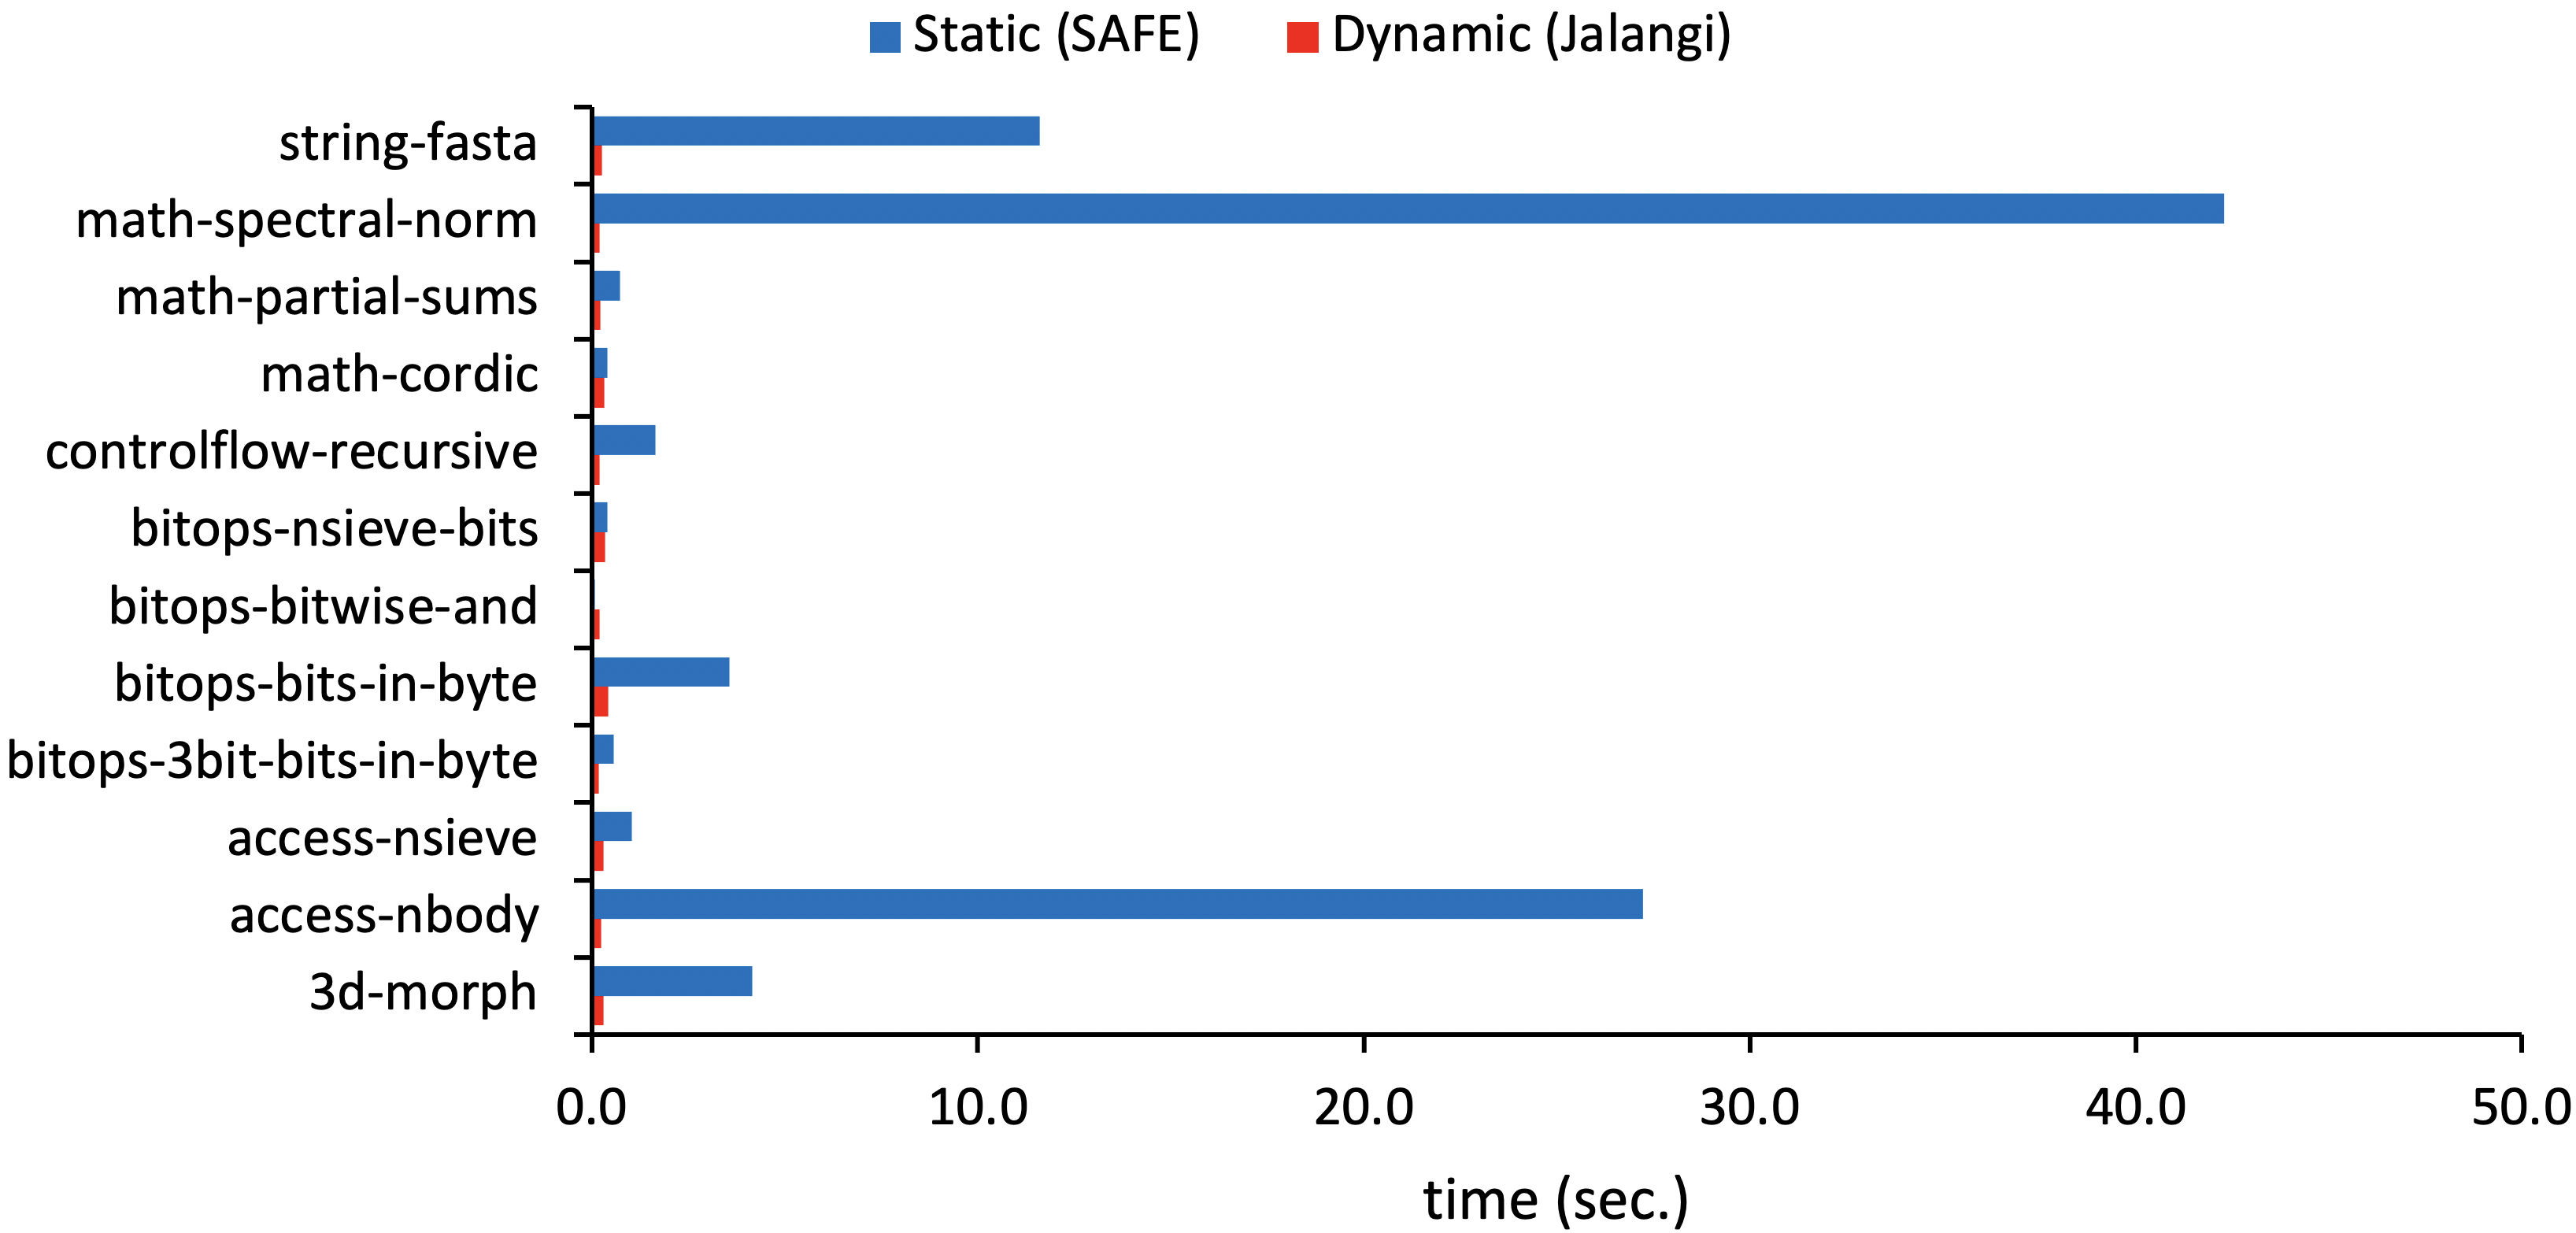
\includegraphics[width=\linewidth]{img/performance_v8v7}
  \vspace*{-2em}
  \caption{Performance of a dynamic analyzer and a static analyzer for a subset
  of the SunSpider benchmark}
  \label{fig:performance}
  \vspace*{-1em}
\end{figure}

To alleviate these problems, researchers have leveraged
dynamic analysis during static analysis.  \inred{Because dynamic
analyzers such as Jalangi~\cite{jalangi} and DLint~\cite{dlint} run on
highly-optimized commercial JavaScript engines while static analyzers run on
their own interpreters, that leads to a great gap in performance.}
Figure~\ref{fig:performance} shows that the dynamic analyzer
Jalangi is 34.8x faster than the static analyzer SAFE for a subset of the
SunSpider benchmark \inred{that is input-independent and deterministic}.
Using high performance dynamic analysis, researchers have
reduced the scope of static analysis~\cite{determinacy, blendedJS} and constructed
initial abstract states~\cite{battles, eha} and automatic modeling of opaque
code~\cite{sra}.

Unfortunately, existing techniques using dynamic analysis for static analysis
have two limitations: 1) they do not fully utilize the high performance of dynamic
analysis, and 2) they sacrifice the soundness of static analysis.  Most of
them are \textit{staged analyses}, which first extract specific
information via dynamic analysis and utilize it in static analysis.
\citet{determinacy} identify determinate expressions that always have the same
values at given program points, \citet{blendedJS} extract dynamic values to
change expressions to certain literals, and Park et al.~\cite{battles,eha} dump
the initial states of a certain host environment or the entry of an event handler.
However, because they do not utilize dynamic analysis as soon as static
analysis begins, they do not get performance benefits since then.  Moreover,
they sacrifice the soundness of static analysis by performing dynamic analysis.
For example, the SRA model~\cite{sra} uses dynamic analysis for opaque code
with abstract arguments during static analysis.  When the abstract arguments
represent an infinite number of values, it randomly samples finite
concrete values for the abstract arguments, which makes the analysis
result unsound due to missing concrete values.

In this paper, we propose a novel technique to fully utilize
the high performance of dynamic analysis for JavaScript static
analysis in a sound manner by using \textit{dynamic shortcuts}.
During static analysis, one can take a dynamic shortcut, which
consists of three parts: 1) converting the current abstract state to
its corresponding \textit{sealed symbolic state}, 2) performing
\textit{sealed symbolic execution} on the sealed symbolic state, and
3) converting the result of the sealed symbolic execution to its
corresponding abstract state.  Our key observation is that we can use
the fast concrete execution for specific program parts while
preserving the soundness if they do not use abstract values.
For example, consider static analysis of the following code:
\begin{lstlisting}[style=myJSstyle,numbers=none]
    var v = ... // an abstract value
    var obj = { p1: v }, y = "p";
    x = obj[y + 1];
\end{lstlisting}
Because \jscode{y + 1} evaluates to \jscode{"p1"},
the third line assigns the abstract value of \jscode{v} stored in
\jscode{obj.p1} to the variable \jscode{x}.
Note that even though \jscode{obj} contains an abstract value \jscode{v},
because the third line does not ``use'' the value of \jscode{v},
we can concretely execute the code.  Based on this observation,
we introduce sealed symbolic execution, which is concrete execution
using \textit{sealed symbolic values}.  A sealed symbolic value is a
representation of an abstract value in symbolic execution; it signals
the end of the current dynamic shortcut when the sealed symbolic
execution tries to access its value.
To evaluate our technique, we implemented $\tool$ using both SAFE
and Jalangi and analyzed 269 official tests of Lodash 4 library.

The contributions of this paper include the following:
\begin{itemize}
\item We present a novel technique for JavaScript static
analysis to leverage the high performance of dynamic analysis using
dynamic shortcuts.  We formally define the technique and prove
its soundness and termination.
\item We actualize the proposed technique in $\tool$, an
extended combination of SAFE and Jalangi.
\item For empirical evaluation, we analyzed 269 official tests of
Lodash 4 library.  The experiment shows that $\tool$ outperforms
SAFE 6.30$\x$ on average.  Moreover, by using dynamic shortcuts
instead of manual modeling for 12 opaque functions,
$\tool$ improves the analysis precision to detect 6 more dead branches on
average.
\end{itemize}

In the remainder of this paper, Section~\ref{sec:motivation} explains the
motivation of this work with a simple example.  Section~\ref{sec:formal}
formalizes the language-agnostic part of the technique in the abstract
interpretation framework.  Then, we extend the formalization with
JavaScript specific features in Section~\ref{sec:javascript}.
Section~\ref{sec:implementation} describes important details of the
$\tool$ implementation.  We explain the evaluation results of $\tool$
with real-world benchmarks in Section~\ref{sec:eval}.
Section~\ref{sec:related} discusses related work and
Section~\ref{sec:conclusion} concludes.

\section{Motivation}\label{sec:motivation}

\begin{figure}[t]
  \centering
  \begin{subfigure}[t]{0.5\textwidth}
    \begin{lstlisting}[style=myJSstyle]
function concat() {
  var length = arguments.length;
  if (!length) return [];
  var args = Array(length - 1),
      array = arguments[0],
      index = length;
  while (index--)
    args[index-1] = arguments[index];
  return arrayPush(
    isArray(array) ? copyArray(array) : [array],
    baseFlatten(args, 1));
}
    \end{lstlisting}
    \vspace*{-1em}
    \caption{Lodash's \jscode{concat} function.}
    \label{fig:concat}
  \end{subfigure}
  \begin{subfigure}[t]{0.5\textwidth}
    \begin{lstlisting}[style=myJSstyle,firstnumber=13]
function changeCountry(G) {
  ...
  if (G.selectedVal === "US" && state) {
    // deterministic arguments of `concat`
    state.items = _.concat([["Other", "Other"]],
      WebinarBase.questions.state.items);
    state.selectedVal = _.head(_.head(C.items));
  }
}
    \end{lstlisting}
    \vspace*{-1em}
    \caption{Load the list of states of the United States.}
    \label{fig:changeCountry}
  \end{subfigure}
  \begin{subfigure}[t]{0.5\textwidth}
    \begin{lstlisting}[style=myJSstyle,firstnumber=22]
function getData(e) {
  var option = ... // option of server connection
  post(option).then(function(e) {
    if (e.total_records && e.total_records > 0) {
      // non-deterministic arguments of `concat`
      this.pastEvents =
        _.concat(this.pastEvents, e.events);
      this.total = e.total_records;
    } else this.noPastData = !0
  })
}
    \end{lstlisting}
    \vspace*{-1em}
    \caption{Load more Zoom events from the server.}
    \label{fig:getData}
  \end{subfigure}
  \vspace*{-1em}
  \caption{Motivating Example: Excerpts from Lodash library and JavaScript codes
  in \code{zoom.us} site.}
  \label{fig:example}
\end{figure}


In this section, we first point out limitations that existing techniques face to
analyze the real-world example described in Figure~\ref{fig:example}.
We then show how our combined analysis increase the analysis scalability and
precision through sealed symbolic execution, seamlessly combined with the original
static analysis.


We excerpt the \jscode{concat} function in Figure~\ref{fig:concat} from Lodash
library~\cite{lodash} (v4.17.20), which is the most popular npm package~\footnote{https://www.npmjs.com/browse/depended}
that \inred{124,562} npm packages depend on.
The \jscode{concat} function creates a new array concatenating given arrays or
values.
It first checks the length of arguments in line 2-3. Then, it stores the first
argument to \jscode{array} in line 5 and copies the remaining arguments to
\jscode{args} in line 7-8.
Finally, it creates a new array by copying the given array via \jscode{copyArray}
or initializing with a single value in line 10, and pushes each element of
\jscode{args} after flattening it via \jscode{baseFlatten} in line 11.


The functions in Lodash are popular to implement common functionalities for
websites as well.
We excerpt two functions \jscode{changeCountry} in Figure~\ref{fig:changeCountry}
and \jscode{getData} in Figure~\ref{fig:getData} from the \code{zoom.us}~\cite{zoom} site.
The website \code{zoom.us} is ranked at \inred{16th} popular web site accroding
to Alexa~\footnote{https://www.alexa.com/siteinfo/zoom.us} in November 2020.
The \jscode{changeCountry} is the example of using \jscode{concat} only with
concrete values.
The \jscode{changeCountry} function is invoked when a user selects his/her
country on the dropdown list in the register page.
When the user selects ``United States of America'', \jscode{changeCountry} calls
the \jscode{concat} function in line 17-18 to prepare the array for
``State/Province'' dropdown list.
The first argument of \jscode{concat} is an array literal \jscode{[["Other",
"Other"]]} and the second one is an array of pairs of abbreviations and names of
the states defined as follows:
\begin{lstlisting}[style=myJSstyle,numbers=none]
WebinarBase.questions.state.items =
  [["AL","Alabama"], ..., ["WY", "Wyoming"]]
\end{lstlisting}
Thus, \jscode{changeCountry} always invokes \jscode{concat} with concrete values.
In the case of \jscode{getData}, \jscode{concat} works with unknown values.
The \jscode{getData} function is invoked when loading more Zoom events in
``Webinars \& Events'' page.
At the first time, initial eight events appear on the page.
For each click of the ``Load More'' button, the \jscode{getData} sends a POST
request to the server and receives data of 8 more events by calling \jscode{concat} in line 28.
As a result, the events list on the page keeps growing by 8.
Both functions, selecting an option of dropdown list and loading more contents
from server-side, are familiar to users.


Existing techniques: static analysis, dynamic analysis, and combined analysis
have limitations to deal with the program containing \jscode{changeCountry} and
\jscode{getData}.
Static analyses of low degrees of context sensitivity tend to cause the
precision loss during analyzing \jscode{concat} function.
The loop in line 7-8 can lead to messing up every property value of args object.
Moreover, \jscode{baseFlatten} has a recursive call that is another challenge
for static analysis.
High degrees of context sensitivity is the promising way, but its computaion
cost is the burden.
Dynamic analyses can show much higher performance for the \jscode{concat} call
by \jscode{changeCountry} than static analyses without any unsoundness and
precision loss.
However, they cannot cover all possible behavior of the \jscode{concat} call
by \jscode{getData} originated by unknown server-side data.
A promising form of combined analysis is dynamically analyzing the call by \jscode{changeCountry}
and statically analyzing the call by \jscode{getData} that is not possible by
existing combined analyses.
User events trigger both functions, the order of function calls is
non-deterministic, so the proper point to divide stages for combined analyses
does not exist.
The syntactic division of the program imposes to choose only one kind of analysis
for the \jscode{concat} function that restricts the benefits of combined analysis.


We present a more flexible and fine-grained method to combine two analyses to
maximize the benefits.

Our observation is

%When the given arguments of a function invokation are concrete values, we can
%perform dynamic analysis instead of static analysis. For example, The
%\jscode{changeCountry} function is invoked when a country different with the
%current one is selected in registration of Zoom meetings.  When the ``United
%States of America'' (USA) is selected, it calls the \jscode{concat} function
%with two pre-defined concrete values as arguments to load USA state information
%in line 17-18.  The first argument is an array literal \jscode{[["Other",
%"Other"]]} and the second one is an array of pairs of abbreviations and names of
%USA states defined as follows:
%\begin{lstlisting}[style=myJSstyle,numbers=none]
%WebinarBase.questions.state.items =
%  [["AL","Alabama"], ..., ["WY", "Wyoming"]]
%\end{lstlisting}
%Moreover, \jscode{this} value is also a concrete value, the Lodash top-level
%object \jscode{\_}.  Thus, we could perform dynamic analysis by invoking the
%\jscode{concat} funciton with \jscode{\_} as \jscode{this} value and above two
%concrete values as arguments.  It increases performance of static analysis by
%skipping the analysis of function call in line 17-18 and utilizing the result of
%dynamic analysis.
%
%Dynamic analysis is still applicable using lazy concrete execution even if the
%arguments are not concrete values.  The \jscode{getData} function is another
%part to use \jscode{concat} function but we can only partially apply dynamic
%analysis in this case.  It is invoked when loading more Zoom events in
%``Webinars \& Events'' page.  At the first time, initial eight events are stored
%in \jscode{this.pastEvents}.  For each click of the ``Load More'' button, the
%\jscode{getData} sends a POST request to the server and receives additional
%event information \jscode{e} in line 24.  Then, eight events in
%\jscode{e.events} are appended to \jscode{this.pastEvents} using the
%\jscode{concat} function in line 27-28.  In this case, arguments are not
%deterministic but dependent on the given data from the server.  However, we know
%that the number of arguments are still deterministically defined as \jscode{2}
%and they are array objects.  Thus, we just invoke the funciton \jscode{concat}
%with \jscode{\_} as \jscode{this} value and two abstract arrays as arguments for
%dynamic analysis.  Then, dynamic analysis is successfully performed in line 2-8
%because it just checks the length of \jscode{arguments} and passes its elements
%to \jscode{array} and \jscode{args}.  Moreover, \jscode{isArray(array)} is also
%able to be evaluated using concrete semantics because we know that \code{array}
%is an abstract array.  Only copying via \jscode{copyArray}, flattening via
%\jscode{baseFlatten}, and pushing via \jscode{arrayPush} utilize the abstract
%semantics.  This is the core idea of lazy concrete execution to maximize the
%part of dynamic analysis during static analysis.

In the remaining section we formally define the combined analysis with sealed
symbolic execution in Section~\ref{sec:formal}.  Then, we explain how to define
the combined analysis for JavaScript programs in Section~\ref{sec:javascript}.

\section{Dynamic Shortcut}\label{sec:formal}

In this section, we formally define the dynamic shortcut with sealed symbolic
execution.  We extend the formalization of abstract interpretation of
\citet{abs-interp-1977, abs-interp-1992} and views-based analysis sensitivity of
\citet{sens-toplas}.


\subsection{Concrete Semantics}

We define a program $\prog$ as a state transition system $(\stset, \trans,
\istset)$.  A program starts with an initial state in $\istset$ and the
transition relation $\trans \subseteq \stset \times \stset$ describes how states
are transformed to other states.  A \textit{collecting semantics} $\sem{\prog} =
\{ \st \in \stset \mid \ist \in \istset \wedge \ist \trans^* \st \}$ consists of
reachable states from initial states of the program $\prog$.  We could calculate
it using the \textit{transfer function} $\transfer: \dom \rightarrow \dom$ as
follows:
\[
  \sem{\prog} = \underset{n \rightarrow \infty}{\lim}{\transfer^n(\ielem)}\\
  \qquad
  \transfer(\elem) = \elem \join \step(\elem)\\
\]
The \textit{concrete domain} $\dom = \powerset{\stset}$ is a complete lattice
with $\cup$, $\cap$, and $\subseteq$ as its join($\join$), meet($\meet$), and
partial order($\order$) operators.  The element $\ielem$ denotes the initial
states $\istset$.  The \textit{one-step execution} $\step: \dom \rightarrow
\dom$ transforms states using the transition relation $\trans$: $\step(\elem) =
\{ \st' \mid \st \in \elem \wedge \st \trans \st' \}$.

\begin{figure}[H]
  \[
    \begin{array}{l}
      \enspace \labdot{0} \; \varx = \;? \; ;  \; \labdot{1}\\
      \enspace \kwif \; (\; \varx \geq 0 \;) \; \labdot{2} \; \varx = \varx ;\\
      \enspace \kwelse \; \labdot{3} \; \varx = -\varx ;  \; \labdot{4}\\
    \end{array}
  \]
  \vspace*{-1em}
  \caption{Conditional branch}
  \label{fig:running-example}
\end{figure}

For example, the code in Figure~\ref{fig:running-example} is a simple program
that applies the mathematical absolute value function to the variable $\varx$.
The question mark $?$ denotes the user input that returns an integer.  States
are pairs of labels and integers $\varx$: $\stset = \labset \times \mathbb{N}$.
The initial states are $\istset = \{ (\lab_0, 0) \}$ which means the program
starts with the variable $\varx$ that stores 0 at $\lab_0$.  If the user input is
$-42$, the program is executed with the following trace:
\[
  (\lab_0, 0) \trans (\lab_1, -42) \trans (\lab_3, -42) \trans (\lab_4, 42)
\]

\subsection{Abstract Interpretation}
The abstract interpretation~\cite{abs-interp-1977, abs-interp-1992}
over-approximates the transfer $\transfer$ to the \textit{abstract transfer
function} $\abstransfer: \absdom \rightarrow \absdom$ to get the
\textit{abstract semantics} $\abssem{\prog}$ in finite iterations as follows:
\[
    \abssem{\prog} = \underset{n \rightarrow
    \infty}{\lim}{(\abstransfer)^n(\iabselem)}\\
\]
We define a \textit{state abstraction} $\dom \galois{\alpha}{\gamma} \absdom$ as
a Galois connection between the concrete domain $\dom$ and an abstract domain
$\absdom$ with a \textit{concretization function} $\gamma$ and an
\textit{abstraction function} $\alpha$.  The initial abstract state $\iabselem
\in \absdom$ represents an abstraction of the initial state set; $\ielem
\subseteq \gamma(\iabselem)$.  The abstract transfer function $\abstransfer:
\absdom \rightarrow \absdom$ is defined as $\abstransfer(\abselem) = \abselem
\join \absstep(\abselem)$ with an \textit{abstract one-step execution}
$\absstep: \absdom \rightarrow \absdom$.  For the sound state abstraction, the
join operator and the abstract one-step execution should satisfy the following
conditions:
\begin{itemize}
  \item $\forall \abselem_0, \abselem_1 \in \absdom. \; \gamma(\abselem_0) \cup
    \gamma(\abselem_1) \subseteq \gamma(\abselem_0 \join \abselem_1)$
  \item $\forall \abselem \in \absdom. \; \absstep \circ \gamma(\abselem) \subseteq
    \gamma \circ \absstep(\abselem)$
\end{itemize}

A simple example abstract domain is $\absdom_\pm = \powerset{\{ -, +, 0 \}}$ with
set operators as domain operators; $-$ denotes negative integers, $+$ positive
integers, and $0$ zero.  If we use it for the code in
Figure~\ref{fig:running-example}, the analysis result becomes $\{ -, +, 0 \}$
because $\varx$ can have any integers at $\lab_1$.


\subsection{Analysis Sensitivity}

Abstract interpretation is often defined with \textit{analysis sensitivity} to
increase the precision of static analysis.  A sensitive abstract domain
$\sabsdom: \viewset \rightarrow \absdom$ is defined with a \textit{view
abstraction} $\viewmap: \viewset \rightarrow \dom$ that provides multiple points
of views for reachable states during static analysis.  It maps a finite number
of views $\viewset$ to sets of states $\dom$. Each view $\view \in \viewset$
represents a set of states $\viewmap(\view)$.
A \textit{sensitive state abstraction} $\dom
\galois{\alpha_\viewmap}{\gamma_\viewmap} \sabsdom$ is a Galois connection between
the concrete domain $\dom$ and the sensitive abstract domain $\sabsdom$ with the
following concretization function:
\[
  \gamma_\viewmap(\sabselem) = \{ \st \in \stset \mid \forall \view \in \viewset.
  \; \st \in \viewmap(\view) \Rightarrow \st \in \gamma \circ \sabselem(\view) \}
\]

With analysis sensitivities, the abstract one-step execution $\sabsstep:
\sabsdom \rightarrow \sabsdom$ is defined as follows:
\[
  \sabsstep(\sabselem) = \lambda \view \in \viewset. \; \underset{\view' \in
  \viewset}{\bigjoin}{\viewtrans{\view'}{\view} \circ \sabselem(\view')}
\]
where $\viewtrans{\view'}{\view}: \absdom \rightarrow \absdom$ is the abstract
semantics of a \textit{view transition} from a view $\view'$ to another view
$\view$.  It should satisfy the following condition for the soundness of the
analysis:
\[
  \forall \abselem \in \absdom. \; \step(\gamma(\abselem) \cap \viewmap(\view'))
  \cap \viewmap(\view) \subseteq \gamma \circ
  \viewtrans{\view'}{\view}(\abselem)
\]

One of the most widely-used analysis sensitivity is \textit{flow sensitivity}
defined with the flow-sensitive view abstraction $\fsviewmap: \labset
\rightarrow \dom$ where
\[
  \forall \lab\in\labset. \; \fsviewmap(\lab) = \{ \st \mid \st = (\lab, \_) \}
\]
If we apply the flow sensitivity for the above example, the analysis result
becomes as follows:
\[
  \begin{array}{|c||c|c|c|c|c|}\hline
    \labset & \lab_0 & \lab_1 & \lab_2 & \lab_3 & \lab_4\\\hline
    \absdom_\pm & 0 & -, +, 0 & +, 0 & - & +, 0\\\hline
  \end{array}
\]


\subsection{Sealed Symbolic Execution}

To handle abstract values in concrete semantics, we define \textit{sealed
symbolic execution} by extending the transition relation $\trans$ as a symbolic
transition relation $\symbtrans$ on symbolic states.  First, we extends the
concrete states $\stset$ to symbolic states with \textit{sealed symbolic values}
$\symbset$.  A symbolic transition relation $\symbtrans \subseteq \symbstset
\times (\symbstset \uplus \{ \excst \})$ is exactly the same with the original
transition relation $\trans$ except when the relation requires the exact value
of sealed symbolic values.  In this case, the symbolic state has the relation a
special exception state $\excst$ to represent that it is impossible to interpret
in a concrete way.  Thus, a symbolic state \textit{always} has a symbolic
transition relation with a single symbolic state, and the sealed symbolic
execution is linear until being terminated or reaching the exception state
$\excst$.

The main difference of sealed symbolic execution with the traditional symbolic
execution~\cite{symbolic} is that it only supports sealed symbolic values
instead of symbolic expressions and path constraints.  For example, the
following trace represents the traditional symbolic execution of the running
example in Figure~\ref{fig:running-example}:
\[
  \begin{array}{r@{~}c@{~}l}
    &&(\lab_2, \symb)[\symb \geq 0] \trans (\lab_4, \symb)[\symb \geq 0]
    \vspace*{-0.5em}\\
    &\rutrans&
    \vspace*{-0.5em}\\
    (\lab_0, 0)[] \trans (\lab_1, \symb)[]&&
    \vspace*{-0.5em}\\
    &\rdtrans&
    \vspace*{-0.5em}\\
    &&(\lab_3, \symb)[\symb < 0] \trans (\lab_4, -\symb)[\symb < 0]\\
  \end{array}
\]
It first assigns a symbolic value $\symb$ to the variable $\varx$ at $\lab_1$.
For the conditional branch, it is forked by creating two symbolic states with
different path conditions $\symb \geq 0$ and $\symb < 0$ for true and false
branches, respectively.  After executing statements $\varx = \varx$ and $\varx =
-\varx$, the variable $\varx$ stores symbolic expressions $\symb$ and $-\symb$ at
$\lab_4$.  However, the sealed symbolic execution stops at $\lab_1$ as follows:
\[
  (\lab_0, 0) \; \symbtrans \; (\lab_1, \symb) \; \symbtrans \; \excst
\]
because the branch requires the actual value of the symbolic value $\symb$.

To freely convert a pair of view and an abstract state to its corresponding
symbolic state and vice versa, we define two domain converters $\symbstset
\galois{\saconverter}{\asconverter} (\viewset \times \absdom)$.  In the
converter $\asconverter$ from abstract states to symbolic states, if an abstract
value $\absval$ represents a singleton value, the function transforms the
abstract value to the corresponding concrete value.  Otherwise, it converts the
abstract value as a symbolic value in a result symbolic state.  Two converters
convert given elements without loss of information:
\[
  \saconverter \circ \asconverter = \asconverter \circ \saconverter = \identity
\]
where $\identity$ denotes the identity function.


\subsection{Dynamic Shortcut}

\begin{figure}[t]
  \centering
  \includegraphics[width=\linewidth]{img/dynamic-shortcut}
  \vspace*{-2em}
  \caption{The diagram for the extended view transition for dynamic shortcut.}
  \vspace*{-1em}
  \label{fig:dynamic-shortcut}
\end{figure}

We define the the abstract interpretation with \textit{dynamic shortcut}, which
is a concrete semantics on sealed symbolic execution.  With dynamic shortcut,
we use the powerset of symbolic states as the domain $\combdom =
\powerset{\symbstset}$, and extend the view transition as follows:
\[
  \begin{array}{l}
    \combviewtrans{\view}{\view'}(\combelem) =\\
    \qquad \{
      \symbst' \mid \symbst \in S \wedge
      \symbst \symbtrans \symbst' \wedge
      \saconverter(\symbst') = (\view', \_)
    \}\\
    \qquad \cup \left\{
    \begin{array}{ll}
      \{ \asconverter \circ \viewtrans{\view}{\view'}(\bigjoin D) \}
      & \text{if} \; D \neq \varnothing\\
      \varnothing & \text{otherwise}\\
    \end{array}
    \right.
  \end{array}
\]
where $S = \combelem\mid_{\checker}$ and $D =
\dot{\saconverter}(\combelem\mid_{\neg\checker})$.  The dot notation $\dot{f}$
denotes the element-wise extended function of a function $f$.  The abstract
interpretation with dynamic shortcut performs one-step symbolic transition for
each symbolic state that passes the filter $\checker$. On the other hand, it
converts remaining symbolic states to the corresponding abstract states, merges
them into a single abstract state, and performs the abstract one-step execution
for the abstract state.

For example, Figure~\ref{fig:dynamic-shortcut} depicts the
diagram of the extended view transition from $\view$ to $\view'$ for dynamic
shortcut.  The element $\combelem$ in $\view$ consists of five symbolic states
from $\nsymbst{1}$ to $\nsymbst{5}$.  The solid box denotes that the corresponding
symbolic state passes the filter $\checker$ and the dotted box denotes that it
does not.  For each symbolic state that passes the filter ($\nsymbst{1}$,
$\nsymbst{2}$, and $\nsymbst{4}$), it applies the symbolic transition $\symbtrans$.
For failed symbolic states ($\nsymbst{3}$ and $\nsymbst{5}$), it applies the
converter $\saconverter$ to convert each of them to the corresponding abstract
state and merges results using the join operator ($\join$).  Then, it utilizes
the abstract semantics via the original view transition
$\viewtrans{\view}{\view'}$ and the converter $\asconverter$ to convert the
result to the corresponding symbolic state.

We could configure when the sealed symbolic execution or the abstract
interpretation is performed based on the definition of the $\checker$ function
and its negation $\neg\checker$.  For example, we could define the $\checker$
that passes only function entry, call, and exit points to perform conversions in
a function level.  However, for the soundness and the termination of the
the abstract interpretation with dynamic shortcut, it should satisfy the
following condition:
\begin{theorem}\label{theorem:shortcut}
  The abstract interpretation with dynamic shortcut is sound and terminates in a
  finite time if its abstract semantics is sound and $\checker$ satisfies the
  following condition:
  \[
    \checker(\symbst) \Rightarrow \symbst \symbtrans^k \excst \wedge
    1 < k \leq N
  \]
  where $N$ is a pre-defined maximum length of the sealed symbolic execution.
\end{theorem}
\inred{We proved Theorem~\ref{theorem:shortcut} using the Kleene's fixed-point
theorem~\cite{kleene} with the finite height of abstract domains. Because of the
page limitation, we omit the proof in this paper and include it in a companion
report~\cite{report}.}

\subsection{Combined Domain}
We now define a \textit{combined domain} of a given sensitive abstract
domain with the {\sealed} domain and its one-step execution.
\begin{definition}[Combined Domain]
  A \textit{combined domain} is $\combdom = \sabsdom \times \symbdom$ and its
  concretization function $\combgamma: \combdom \rightarrow \dom$ and join
  operator are defined as follows:
  \begin{align}
    \combgamma((\sabselem, \symbelem)) &= \sgamma(\sabselem) \cup
      \symbgamma(\symbelem)\\
    (\sabselem, \symbelem) \join ({\sabselem}', \symbelem') &= (\sabselem \join
      {\sabselem}', \symbelem \cup \symbelem')
  \end{align}
\end{definition}

Before defining the one-step execution for the combined domain, we introduce
\textit{analysis elements} to easily configure different types of abstract
states in the sensitive abstract domain and the {\sealed} domain.
\begin{definition}[Analysis Elements]\label{def:aelem}
  An \textit{analysis element} $\aelem \in \aelemset = (\viewset \times \absdom)
  \uplus (\absimapset \times \symbstset)$ is either 1) a pair of a view and an
  abstract state in a sensitive abstract domain $\sabsdom$, or 2) a pair of an
  abstract instantiation map and a {\sealed} state in a {\sealed}
  domain $\symbdom$.  Its concretization function $\aelemgamma:
  \aelemset \rightarrow \dom$ is defined as follows:
  \[
    \aelemgamma(\aelem) = \left\{
      \begin{array}{ll}
        \viewmap(\view) \cap \gamma(\abselem) & \text{if} \; (\view, \abselem) = \aelem\\
        \instant{\symbst}{\absimap} & \text{if} \; (\absimap, \symbst) = \aelem\\
      \end{array}
    \right.
  \]
\end{definition}

\begin{figure*}[t]
  \centering
  \begin{subfigure}[t]{0.15\textwidth}
    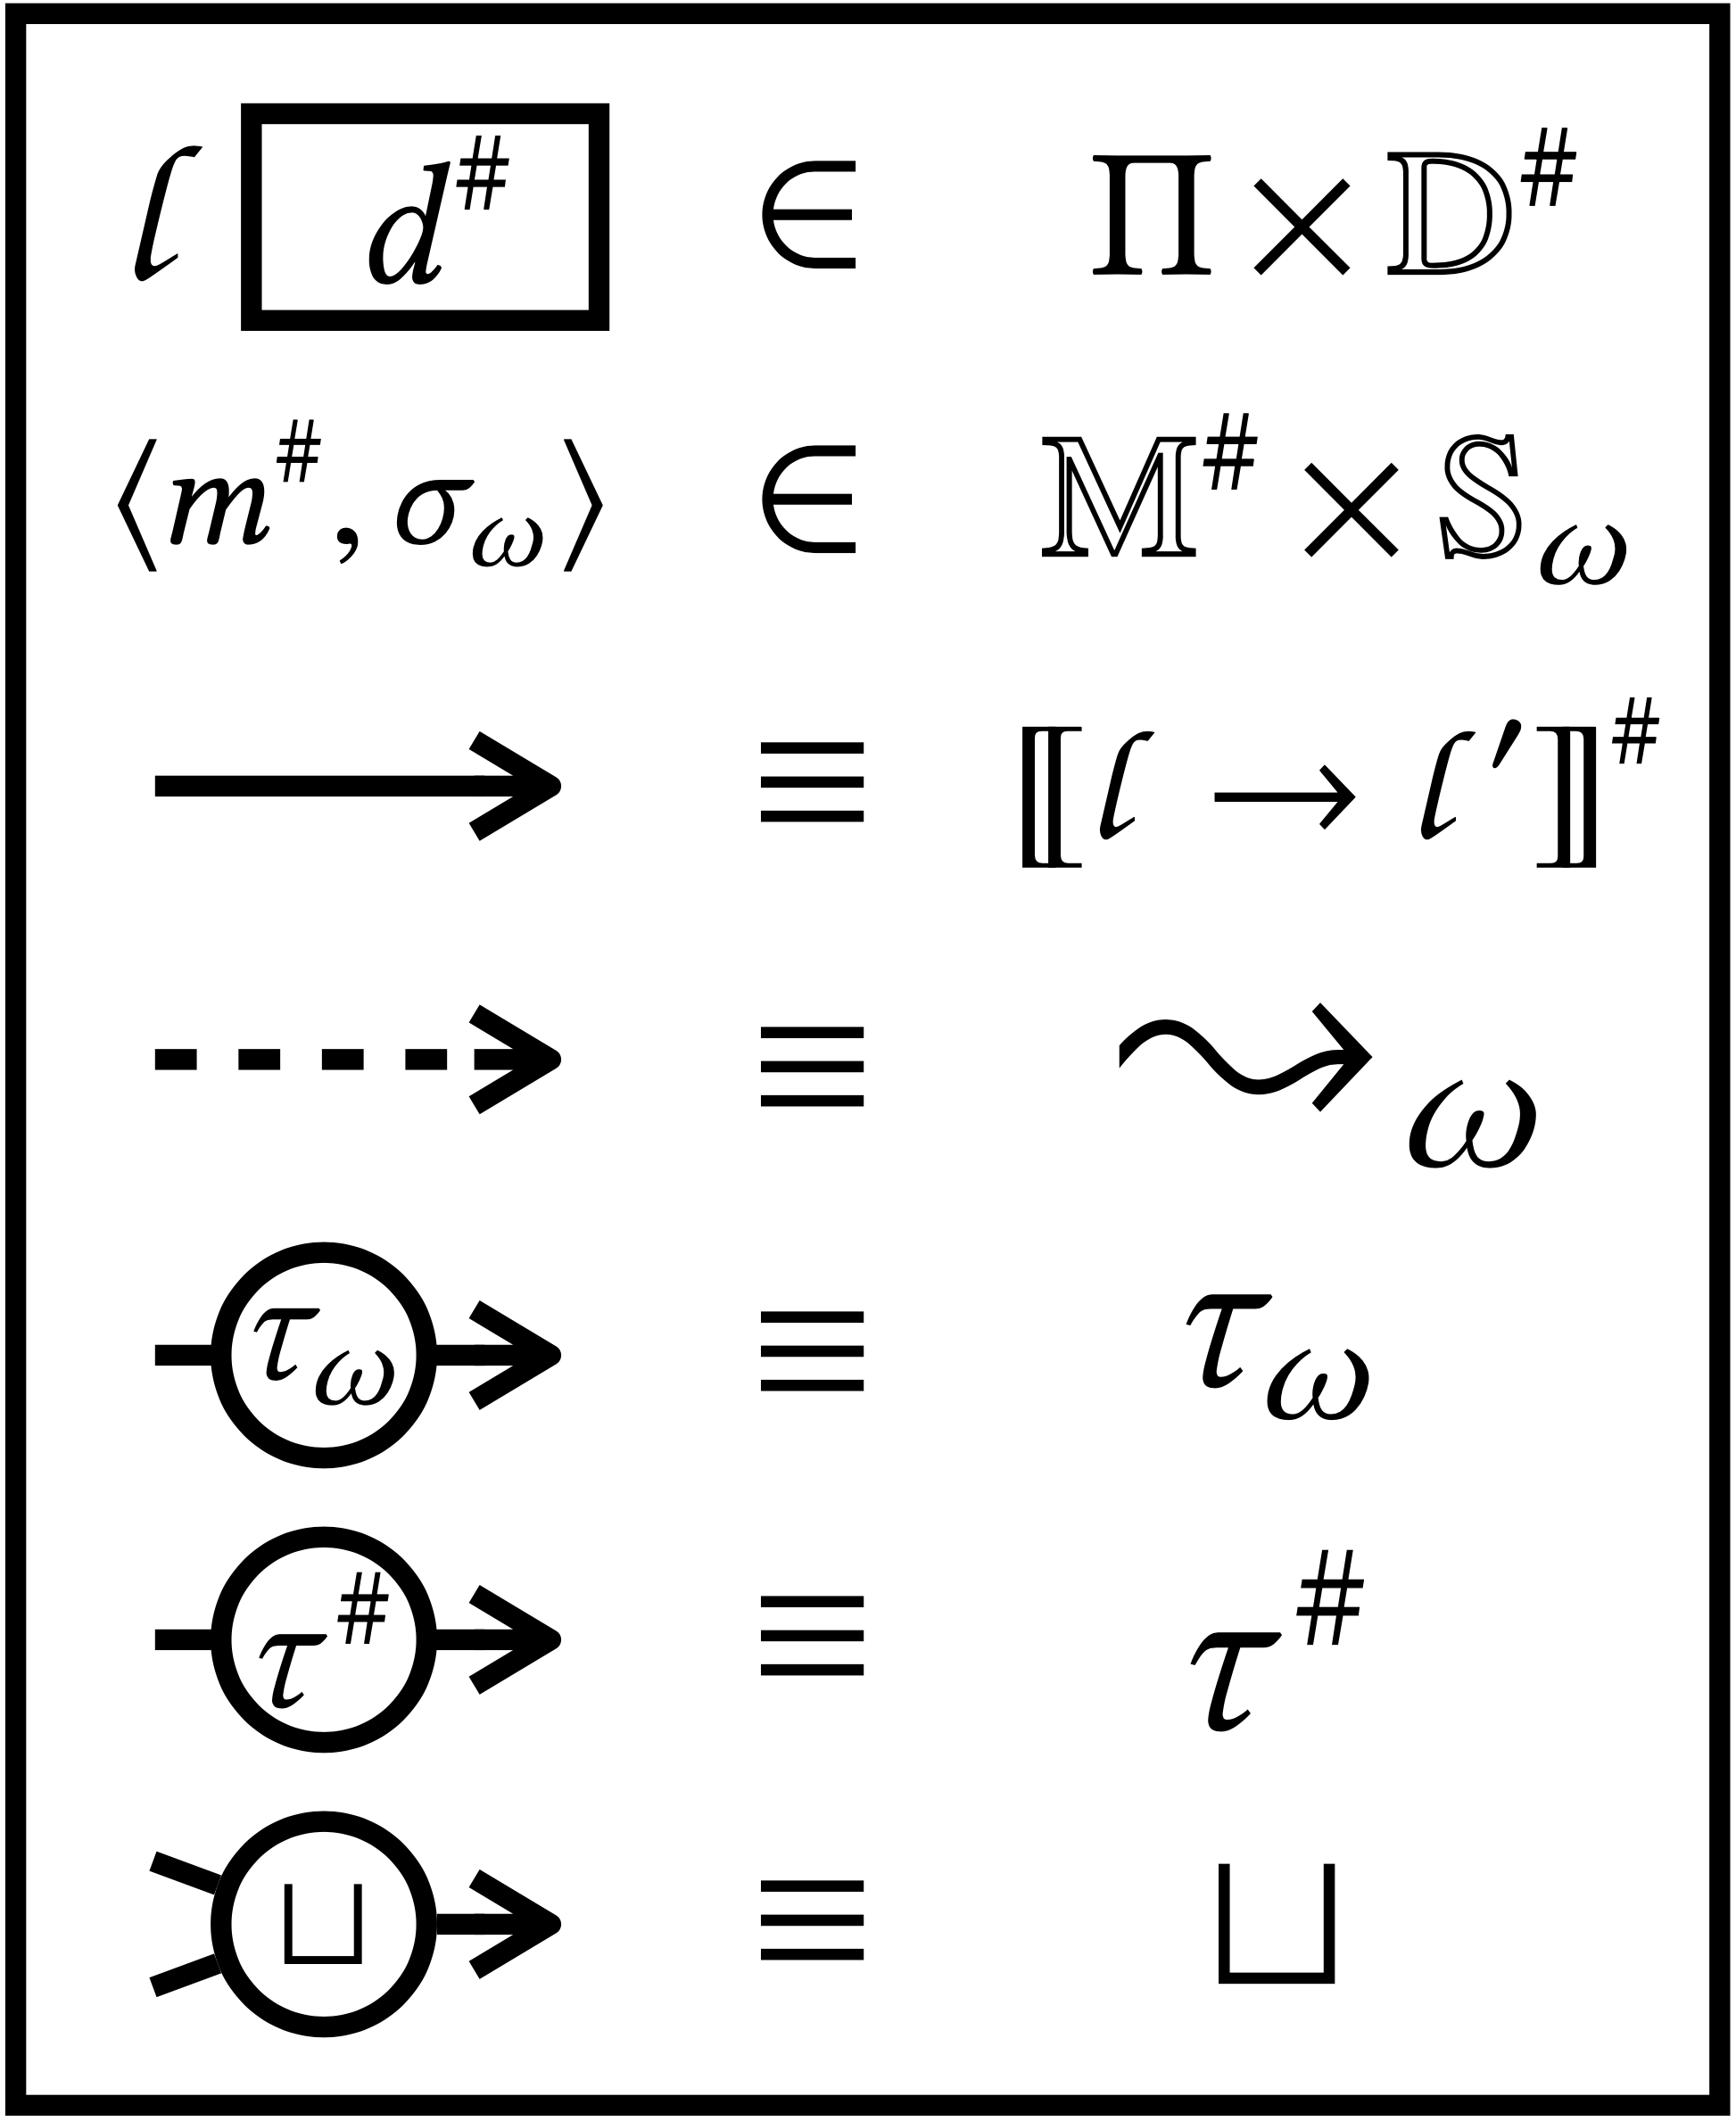
\includegraphics[height=3.2cm]{../img/listing}
    \caption{Notations}
    \label{fig:ds-example1}
  \end{subfigure}
  \quad
  \begin{subfigure}[t]{0.23\textwidth}
    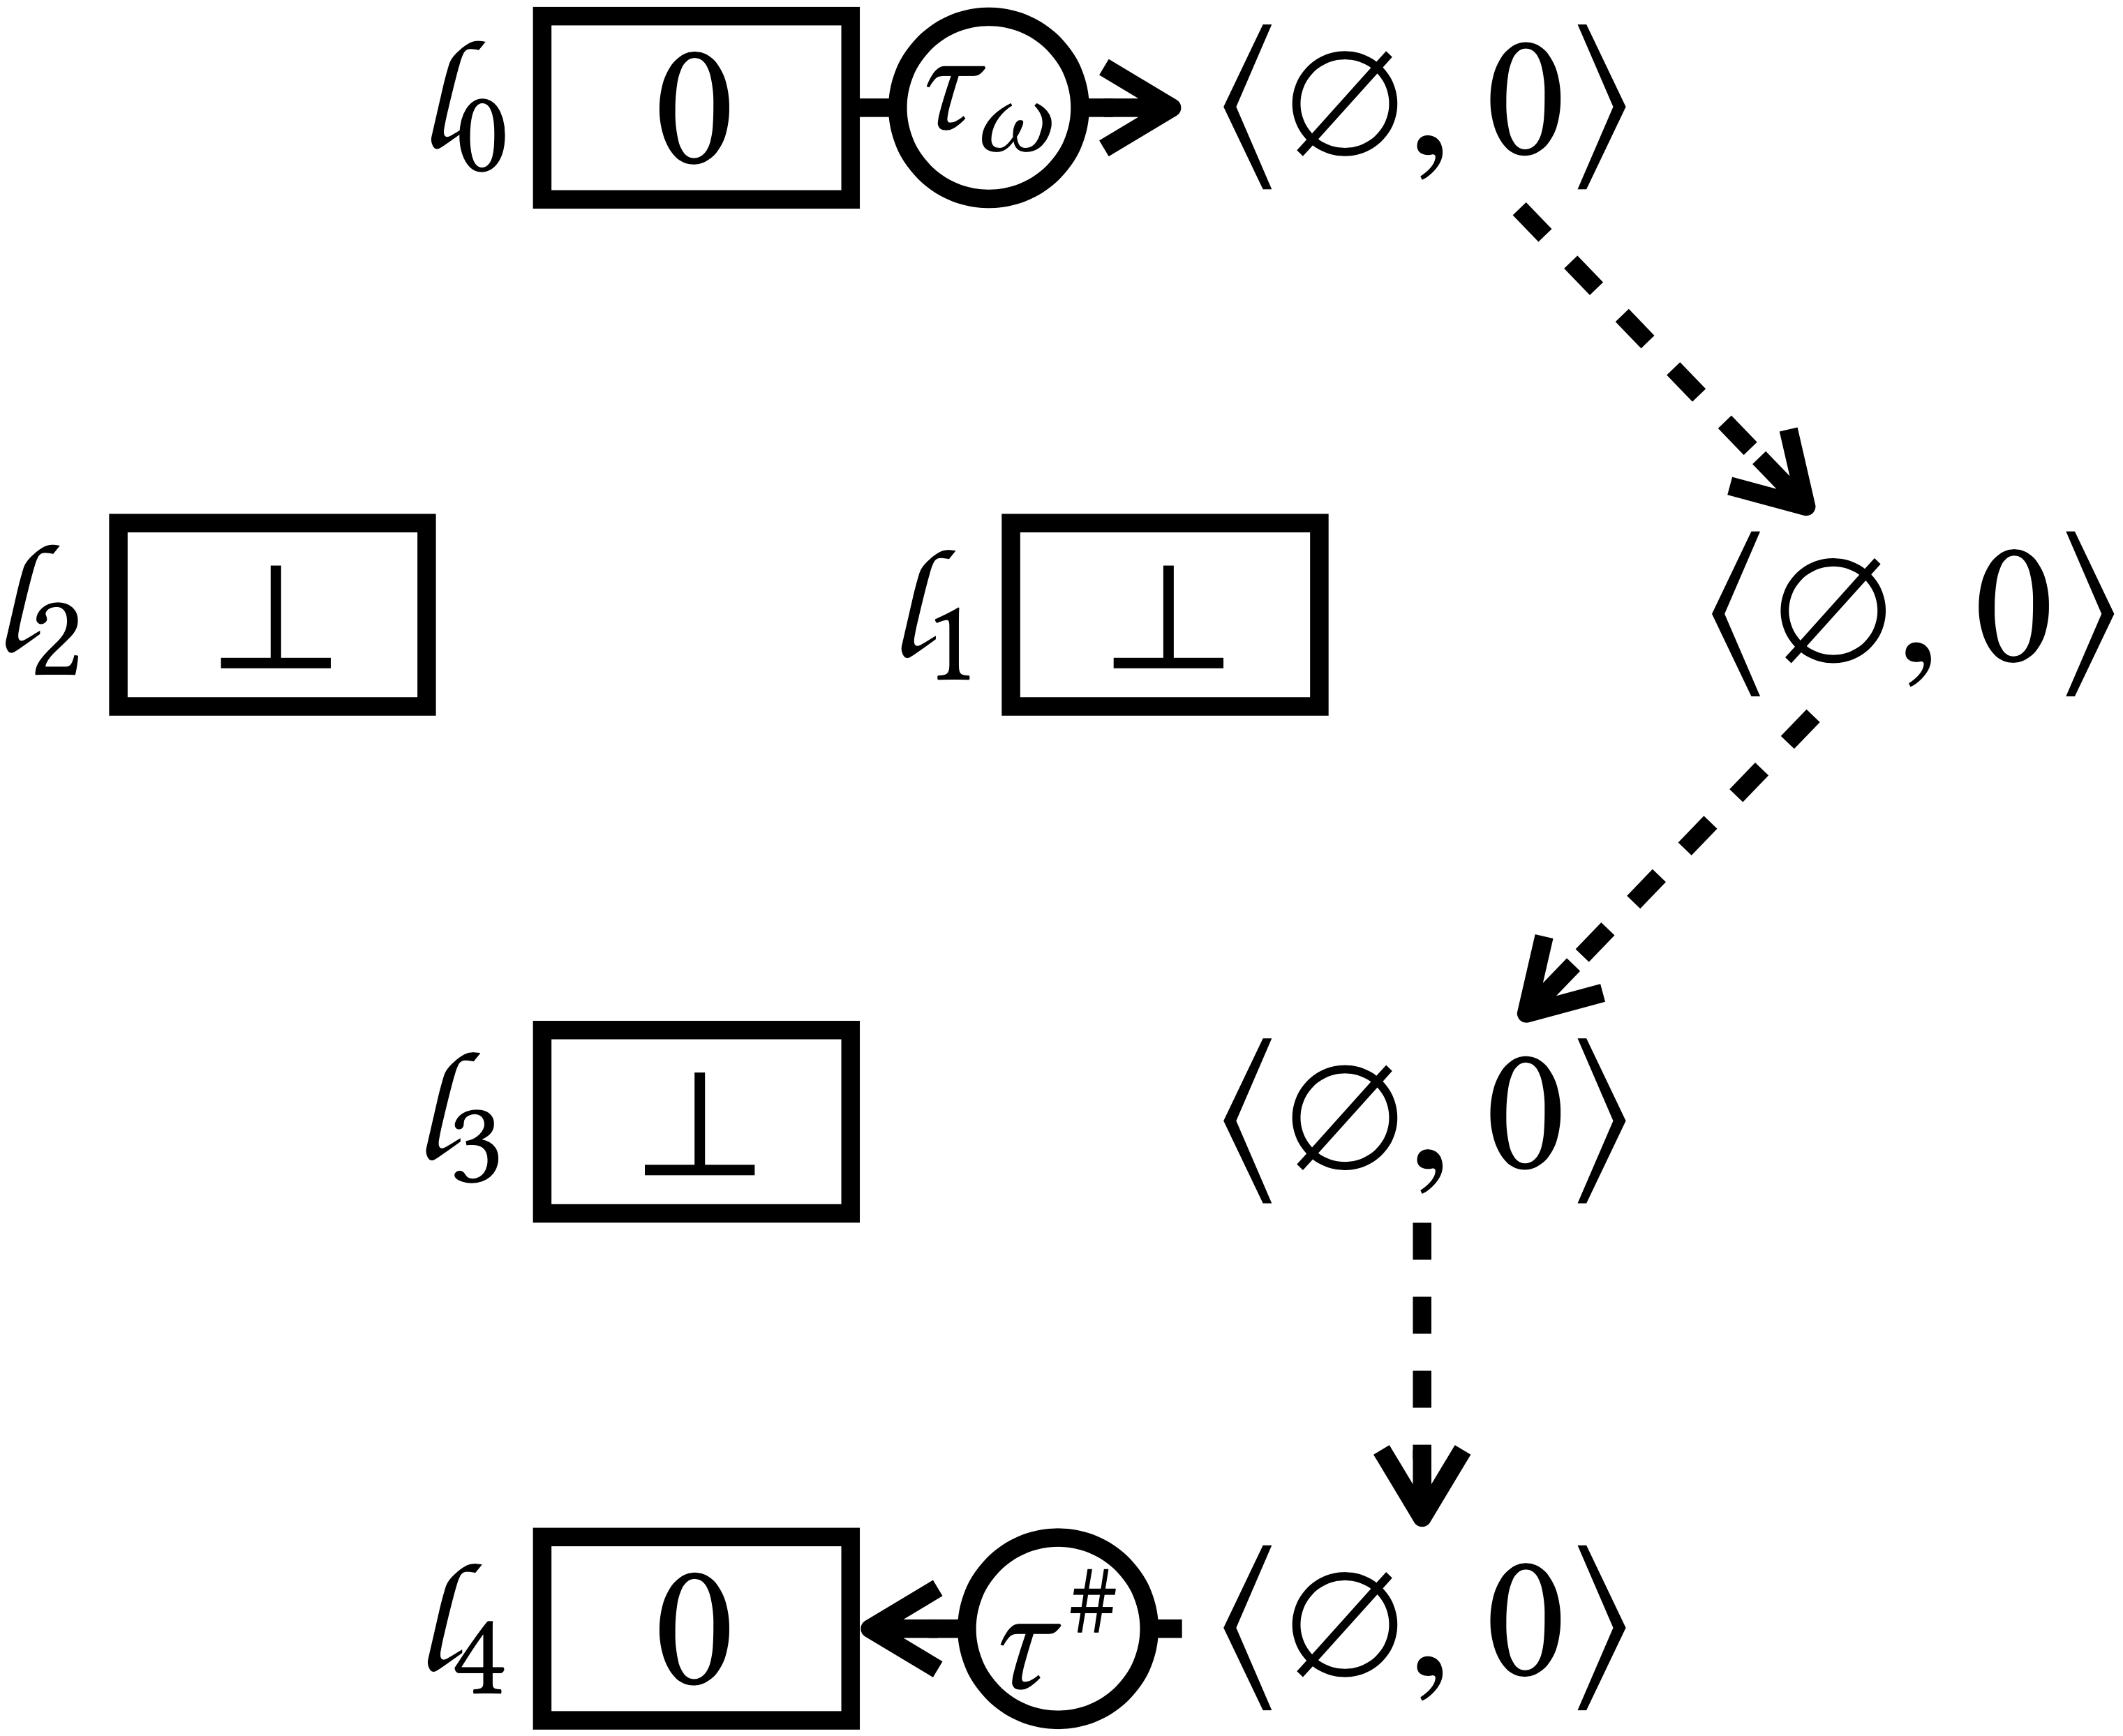
\includegraphics[height=3.2cm]{../img/path-1}
    \caption{$\varx = 0$}
    \label{fig:ds-example2}
  \end{subfigure}
  \begin{subfigure}[t]{0.28\textwidth}
    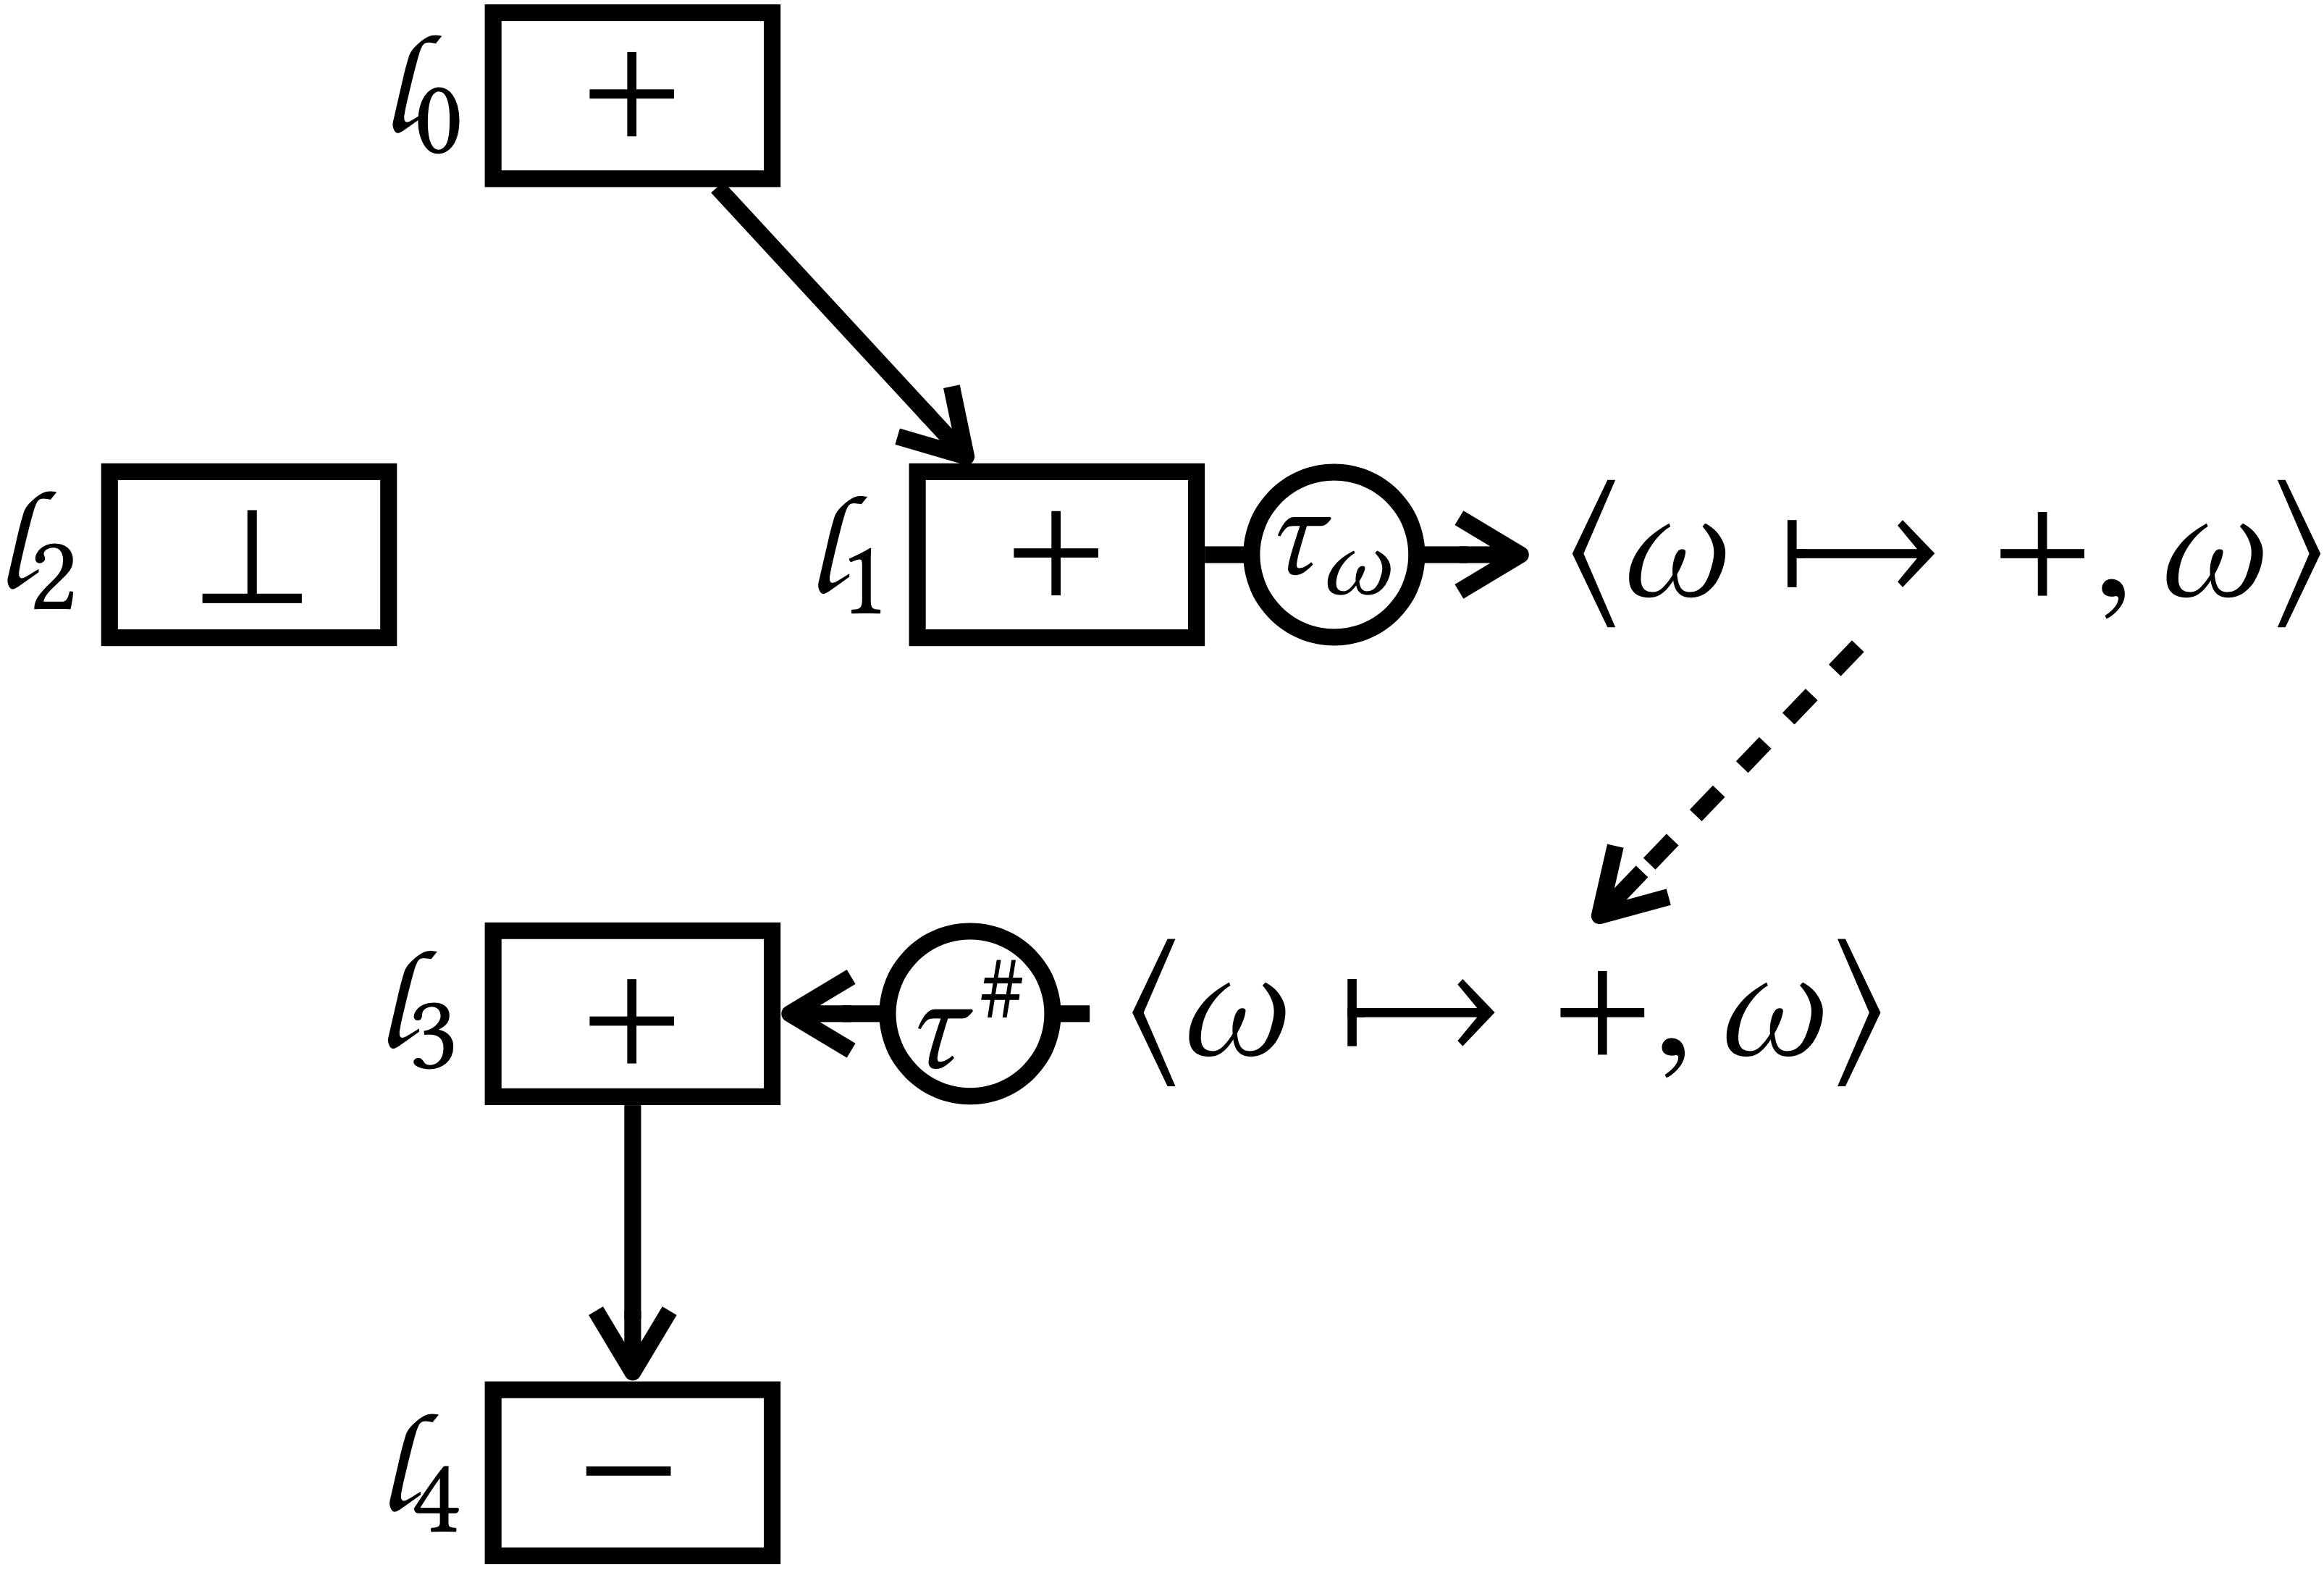
\includegraphics[height=3.2cm]{../img/path-2}
    \caption{$\varx > 0$}
    \label{fig:ds-example3}
  \end{subfigure}
  \begin{subfigure}[t]{0.28\textwidth}
    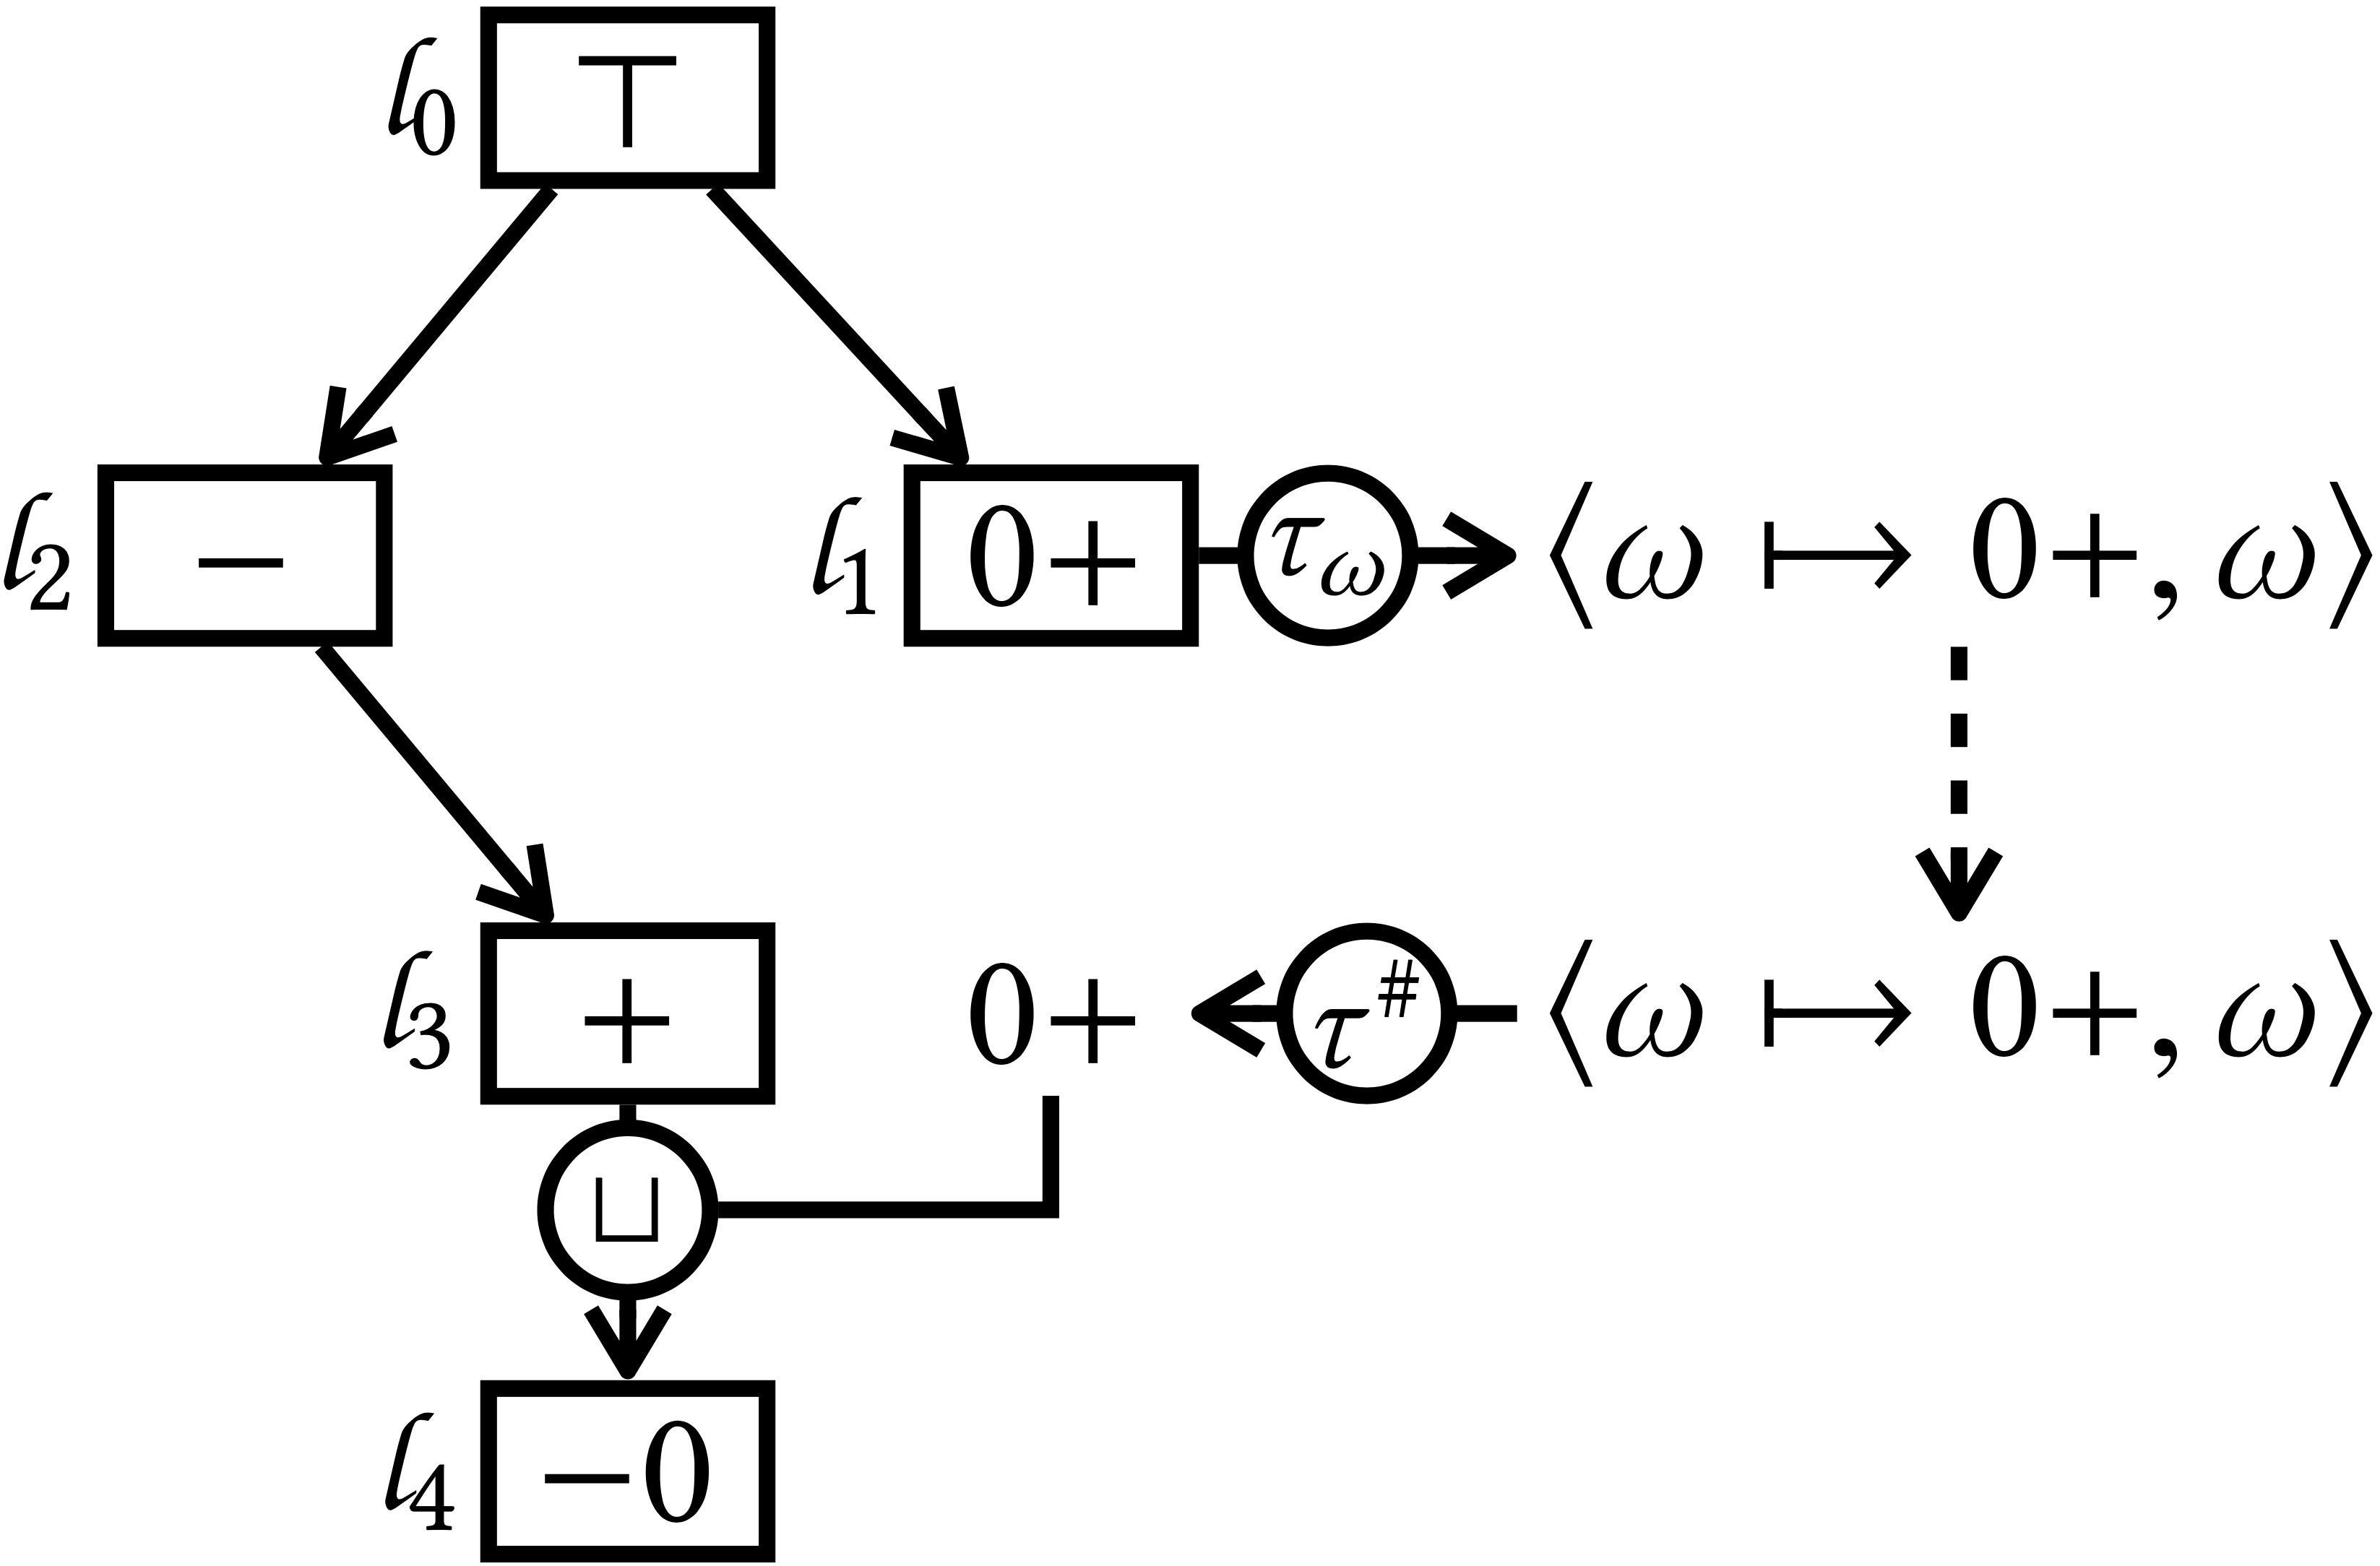
\includegraphics[height=3.2cm]{../img/path-3}
    \caption{$\varx \in \mathbb{N}$}
    \label{fig:ds-example4}
  \end{subfigure}
  \caption{Abstract interpretation using a combined domain for the running
  example with different initial values for $\varx$.}
  \label{fig:ds-examples}
\end{figure*}

Moreover, to freely convert between different kinds of analysis elements, we define two converters:
\begin{align}
  \asconverter & : (\viewset \times \absdom) \hookrightarrow
    (\absimapset \times \symbstset)\\
  \saconverter & : (\viewset \times
    \absdom) \leftarrow (\absimapset \times \symbstset)
\end{align}
While the converter $\saconverter$ is total, the other one $\asconverter$ is
\textit{partial}. Thus, it is possible to convert an analysis element
$(\view, \abselem)$ in a sensitive abstract domain to another analysis element in
a {\sealed} domain only if the convert $\asconverter$ is defined: $(\view,
\abselem) \in \Dom(\asconverter)$.  In addition, they should convert given
analysis elements without loss of information for all $\aelem \in \aelemset$:
\[
  \asconverter(\aelem) = \aelem' \Rightarrow \left\{
  \begin{array}{l}
    \aelem = \saconverter(\aelem')\\
    \aelemgamma(\aelem) = \aelemgamma(\aelem')\\
  \end{array}
  \right.
\]

Now, we define the \textit{combined one-step execution} $\combstep: \combdom
\rightarrow \combdom$ with two converters $\asconverter$ and $\saconverter$.
It consists of two steps: 1) the \textit{\reformname} step converts
analysis elements if a new {\sealed} execution starts or an
existing one stops, and 2) the \textit{execution} step performs execution of each
analysis element using the abstract one-step execution $\sabsstep$ in the sensitive
abstract domain and the {\sealed} one-step execution $\symbstep$ in the {\sealed} domain.
\begin{definition}[Combined One-Step Execution]
A \textit{combined one-step execution} $\combstep: \combdom \rightarrow
\combdom$ is define as follows:
  \[
    \combstep(\combelem) = (\sabsstep(\sabselem), \symbstep(\symbelem))
  \]
where $(\sabselem, \symbelem) = \reform(\combelem)$.
\end{definition}

From a given combined state $\combelem$, the $\reform$ function makes analysis elements
and converts them if a new {\sealed} execution
begins or an existing {\sealed} execution terminates.
Specifically, for an analysis element $(\view, \abselem)$ in the sensitive abstract domain,
if the converter $\asconverter$ is defined for it, $\reform$ introduces a new {\sealed} execution
by converting the analysis element to its corresponding one $(\absimap, \symbst) =
\asconverter((\view, \abselem))$ in the {\sealed} domain.
On the other hand, for an analysis element $(\absimap, \symbst)$ in the {\sealed} domain,
if it does not have any {\sealed} states to transit to, $\symbst \symbtrans \excst$,
the {\sealed} execution for $(\absimap, \symbst)$ terminates.
It converts the analysis element to its corresponding one $(\view, \abselem) =
\saconverter((\absimap, \symbst))$ in the sensitive abstract domain and
merges the current abstract state stored in $\view$ with $\abselem$.

To formally define the $\reform$ function, we first define a $\areform$ function
for analysis elements using two converters.
\begin{definition}[$\areform$]\label{def:areform}
  The function $\areform: \aelemset \rightarrow \aelemset$ for analysis elements
  is defined as follows:
  \[
    \areform(\aelem) = \left\{
      \begin{array}{ll}
        \asconverter(\aelem)
        & \text{if} \; \aelem = (\view, \abselem) \wedge \aelem \in
        \Dom(\asconverter)\\
        \saconverter(\aelem)
        & \text{if} \; \aelem = (\absimap, \symbst) \wedge \symbst \symbtrans
        \bot\\
        \aelem
        & \text{Otherwise}
      \end{array}
    \right.
  \]
\end{definition}
\begin{definition}[$\reform$]\label{def:reform}
  The \reformname function $\reform: \combdom \rightarrow \combdom$ for combined
  states is defined as follows:
  \[
    \reform((\sabselem, \symbelem)) = \left(
      \lambda \view. \bigjoin \{ \abselem \!\mid\! (\view, \abselem) \in E \},
      E \cap (\absimapset \times \symbstset)
    \right)
  \]
  where
  \[
    E = \dot{\areform}(\{ (\view, \sabselem(\view)) \mid \view \in \viewset \} \cup \symbelem)
  \]
and the dot notation $\dot{f}$ denotes the element-wise extended function of a
function $f$.
\end{definition}


\subsection{Examples}
Now, we show examples of abstract interpretation with a combined domain.
Figure~\ref{fig:ds-examples} depicts the flow of analysis for the running
example in Figure~\ref{fig:running-example} with three different initial sets of
values for the variable $\varx$.  In this example, we use the abstract domain
$\{ -, 0, + \}$ for integers stored in $\varx$ as introduced in
Section~\ref{sec:ai}, and the \textit{flow sensitivity} that utilizes the
labels of states as their views as introduced in Section~\ref{sec:sens}.
For brevity, we use concatenation of abstract values so that
$-0$ denotes the set $\{ -, 0 \}$.

Figure~\ref{fig:ds-examples}(a) presents notations used in each graph. A solid
box denotes an analysis element that is a pair of a label $\lab$ and an abstract
state $\abselem$.  A pair enclosed by angle brackets denotes an analysis
element that is a pair of an abstract instantiation map $\absimap$ and a {\sealed}
state $\symbst$.  In fact, the {\sealed} state part (right) of
each pair in graphs contains only the value of the variable of $\varx$ without
its label.  For brevity, we represent its label by locating it next to
a node with its label.  A solid line is a view transition
$\viewtrans{\lab}{\lab'}$ from a label $\lab$ to another one $\lab'$.  A dotted
line is a {\sealed} transition $\symbtrans$.  Three solid lines with
circled labels denote two converters $\saconverter$, $\asconverter$ and the join
operator $\join$.

Figure~\ref{fig:ds-examples}(b) shows the analysis with the combined domain when
the initial value of $\varx$ is $0$.  First, in the \reformname step,
the converter $\asconverter$ converts the analysis element $(\lab_0, 0)$ to
another analysis element $\langle \varnothing, 0 \rangle$ with the label
$\lab_0$.  It does not introduce any {\sealed} values because
the value represents only a single value.  Until the end of the program, the
{\sealed} execution from $\langle \varnothing, 0 \rangle$ successfully
continues.  Because there is no more possible {\sealed} transition for the
{\sealed} state $\langle \varnothing, 0 \rangle$ with $\lab_4$,
it is converted to $(\lab_4, 0)$ via the converter $\saconverter$.

Instead of a single value, assume that the initial value of $\varx$ is one of
any positive integers.  Figure~\ref{fig:ds-examples}(c) describes the analysis
flow for the case.  The initial abstract value at the label $\lab_0$ is
$+$ and it is impossible to convert it to any {\sealed} values because the
next program statement requires the actual value stored in the variable $\varx$
for the branch condition $\varx \geq 0$.  Thus, it performs view transition
$\viewtrans{\lab_0}{\lab_1}$ from the label $\lab_0$ to another one $\lab_1$ for
the abstract value $+$ and the result is also $+$.  Now, the analysis element
$(\lab_1, +)$ can be converted to $\langle \symb \mapsto +, \symb \rangle$
with the label $\lab_1$.  This {\sealed} execution step terminates in the
label $\lab_3$ because the next statement is $\varx = -\varx$ and the negation
operator requires the actual value of $\varx$.  It is converted to $(\lab_3, +)$ via $\saconverter$,
performs the view transition, and results in $(\lab_4, -)$.

For the last case, we assume that all integers are possible for the initial
value of the variable $\varx$ as described in Figure~\ref{fig:ds-examples}(d).
While it reaches the false branch in the label $\lab_2$ unlike previous cases,
it cannot perform dynamic shortcuts because the statement in the false
branch is $\varx = -\varx$, which requires the actual value of $\varx$.
At the label $\lab_3$, there are two analysis
elements: 1) $(\lab_3, +)$ introduced by the view transition from the label $\lab_2$
with $-$, and 2) $\langle \symb \mapsto 0+, \symb \rangle$ with $\lab_3$
introduced by {\sealed} execution started at $\lab_1$.  Since it
is not possible to perform {\sealed} execution for both elements, the
second one is converted to $(\lab_3, 0+)$ and merged with $+$ at $\lab_3$ via the
join operator $\join$.  Finally, the view transition
$\viewtrans{\lab_3}{\lab_4}$ from $\lab_3$ to $\lab_4$ is performed to the
merged abstract state $0+$ and the result is $-0$.

\subsection{Soundness and Termination}
The converter $\asconverter$ and the {\sealed} transition $\symbtrans$ are
keys to configure the introduction and termination of {\sealed}
execution.  To ensure the \textit{soundness} and \textit{termination} of an
abstract interpretation defined with a combined domain of a sensitive abstract
domain and a {\sealed} domain, the following conditions should hold.

\begin{theorem}[Soundness and Termination]\label{theorem:shortcut}
An abstract interpretation with dynamic shortcuts is \textbf{sound} and
\textbf{terminates} in a finite time if:
  \begin{itemize}
    \item the abstract transfer function $\abstransfer$ is sound,
    \item the sensitive abstract domain $\sabsdom$ has a finite height,
    \item the {\sealed} transition $\symbtrans$ is valid, and
    \item there exists $N < \infty$ such that
      \[
        \forall \aelem \in \aelemset. \; \asconverter(\aelem) = (\absimap,
        \symbst) \Rightarrow \symbst
        \symbtrans^k \excst \wedge 1 < k \leq N
      \]
  \end{itemize}
\end{theorem}

To formally prove Theorem~\ref{theorem:shortcut}, we assume that its all
conditions are hold and rephrase the \textit{soundness} as
Theorem~\ref{theorem:soundness} and \textit{termination} as
Theorem~\ref{theorem:termination}.

\subsubsection{Soundness}

\begin{theorem}[Soundness]\label{theorem:soundness}
  The abstract interpretation using the combined domain $\combdom$ is
  \textbf{sound} if
  \begin{equation}\label{equ:sound-join}
    \forall \combelem_0, \combelem_1 \in \combdom. \; \combgamma(\combelem_0) \cup
    \combgamma(\combelem_1) \subseteq \combgamma(\combelem_0 \join \combelem_1)
  \end{equation}
  \begin{equation}\label{equ:sound-combstep}
    \forall \combelem \in \combdom. \; \step \circ \combgamma(\combelem) \subseteq
    \combgamma \circ \combstep(\combelem)\\
  \end{equation}
\end{theorem}
\begin{proof}
  First, we prove that the abstract transfer function $\combtransfer: \combdom
  \rightarrow \combdom$ defined as $\combtransfer(\combelem) = \combelem \join
  \combstep(\combelem)$ is sound
  \[
    \begin{array}{rcll}
      \transfer \circ \combgamma(\combelem)
      &=& \combgamma(\combelem) \cup \step \circ \combgamma(\combelem)\\
      &\subseteq& \combgamma(\combelem) \cup \combgamma \circ \combstep(\combelem)
      & (\because \; \text{condition~(\ref{equ:sound-combstep})})\\
      &\subseteq& \combgamma(\combelem \join \combstep(\combelem))
      & (\because \; \text{condition~(\ref{equ:sound-join})})\\
      &=& \combgamma \circ \combtransfer(\combelem)\\
    \end{array}
  \]
  Then, the abstract semantics $\combsem{\prog} = \underset{n \rightarrow
  \infty}{\lim}{(\combtransfer)^n(\icombelem)} $ is also sound because it is
  defined with a sound abstract transfer function $\combtransfer$ using the
  combined one-step execution $\combstep$.
\end{proof}

Now, we should show that two conditions about the soundness of the join
operator (\ref{equ:sound-join}) and the soundness of the combined one-step
execution (\ref{equ:sound-combstep}) in Theorem~\ref{theorem:soundness} hold.

First, we prove the soundness of the join operator (\ref{equ:sound-join}) in
Lemma~\ref{lemma:sound-join}.
\begin{lemma}[Soundness of $\join$]\label{lemma:sound-join}
  \[
    \forall \combelem_0, \combelem_1 \in \combdom. \; \combgamma(\combelem_0) \cup
    \combgamma(\combelem_1) \subseteq \combgamma(\combelem_0 \join \combelem_1)
  \]
\end{lemma}
\begin{proof}
  \[
    \begin{array}{cl}
      \multicolumn{2}{l}{
        \combgamma((\sabselem, \symbelem)) \cup \combgamma((\sabselem', \symbelem'))
      }\\
      =& \sgamma(\sabselem) \cup \symbgamma(\symbelem)
      \cup \sgamma(\sabselem') \cup \symbgamma(\symbelem')\\
      =& (\sgamma(\sabselem)\cup \sgamma(\sabselem'))
      \cup (\symbgamma(\symbelem) \cup \symbgamma(\symbelem'))\\
      \subseteq& \sgamma(\sabselem \join \sabselem')
      \cup (\symbgamma(\symbelem) \cup \symbgamma(\symbelem'))\\
      & \multicolumn{1}{r}{(\because \; \sabsdom \; \text{is sound})}\\
      =& \sgamma(\sabselem \join \sabselem')
      \cup \symbgamma(\symbelem \cup \symbelem')\\
      =& \combgamma((\sabselem \join \sabselem', \symbelem \cup \symbelem'))\\
      =& \combgamma((\sabselem, \symbelem) \join (\sabselem', \symbelem'))\\
    \end{array}
  \]
\end{proof}

For the condition (\ref{equ:sound-combstep}), we first prove two properties of the
$\reform$ function in Lemma~\ref{lemma:reform}.  Using the properties, we prove
the soundness of the sealed one-step execution in
Lemma~\ref{lemma:sound-symbstep}.  Finally, we prove the soundness of the
combined one-step execution (\ref{equ:sound-combstep}) in
Lemma~\ref{lemma:sound-combstep}.

\begin{lemma}[Properties of $\reform$]\label{lemma:reform}
  For a given combined state $\combelem \in \combdom$, the $\reform$ function
  satisfies the following two properties:
  \begin{itemize}
    \item $\combgamma(\combelem) \subseteq \combgamma \circ \reform(\combelem)$
    \item $\forall (\absimap, \symbst) \in \symbelem. \; \exists \symbst' \in
      \symbstset.  \; \text{s.t.} \; \symbst \symbtrans \symbst'$
  \end{itemize}
  where $(\sabselem, \symbelem) = \reform(\combelem)$
\end{lemma}
\begin{proof}
  \[
    \fbox{$\combgamma(\combelem) \subseteq \combgamma \circ \reform(\combelem)$}
  \]
  \[
    \begin{array}{cl}
      \multicolumn{2}{l}{\combgamma((\sabselem, \symbelem))}\\
      =& \sgamma(\sabselem) \cup \symbgamma(\symbelem)\\

      =& \left( \underset{\view \in \viewset}{\bigcup} {\viewmap(\view) \cap
      \gamma \circ \sabselem(\view)} \right) \cup \left( \underset{(\absimap,
      \symbst) \in \symbelem}{\bigcup} \instant{\symbst}{\absimap} \right) \\

      =& \left( \underset{\view \in \viewset}{\bigcup} \aelemgamma((\view,
      \sabselem(\view))) \right) \cup \left( \underset{(\absimap, \symbst) \in
      \symbelem}{\bigcup} \aelemgamma((\absimap, \symbst)) \right) \\

      =& \dot\aelemgamma(\{ (\view, \sabselem(\view)) \mid \view \in \viewset \}
      \cup \symbelem)\\

      =& \dot\aelemgamma(\dot{\areform}(\{ (\view, \sabselem(\view)) \mid \view
      \in \viewset \} \cup \symbelem))\\

       & \multicolumn{1}{r}{\because \; (\text{Trivially,} \; \forall \aelem \in
       \aelemset.  \; \aelemgamma(\aelem) = \aelemgamma \circ \areform(\aelem))}\\

      =& \dot\aelemgamma(E)\\
       & \multicolumn{1}{r}{\because \; (\text{See the definition of $E$ in
       Definition~\ref{def:reform}})}\\
    \end{array}
  \]
  \[
    \begin{array}{cl}
      =& \left( \underset{(\view, \abselem) \in E}{\bigcup} \aelemgamma((\view,
      \abselem)) \right) \cup \left( \underset{(\absimap, \symbst) \in
      E}{\bigcup} \aelemgamma((\absimap, \symbst)) \right)\\

      =& \left( \underset{(\view, \abselem) \in E}{\bigcup} \viewmap(\view) \cap
      \gamma(\abselem) \right) \cup \left( \underset{(\absimap, \symbst) \in
      E}{\bigcup} \instant{\symbst}{\absimap} \right)\\

      =& \left( \underset{\view \in \viewset}{\bigcup} { \underset{(\view,
      \abselem) \in E}{\bigcup} \viewmap(\view) \cap \gamma(\abselem) } \right)
      \cup \left( \underset{(\absimap, \symbst) \in E}{\bigcup}
      \instant{\symbst}{\absimap} \right)\\

      =& \left( \underset{\view \in \viewset}{\bigcup} {\viewmap(\view) \cap
        \left(\underset{(\view, \abselem) \in
      E}{\bigcup}{\gamma(\abselem)}\right)} \right) \cup \left(
      \underset{(\absimap, \symbst) \in E}{\bigcup} \instant{\symbst}{\absimap}
      \right)\\

      \subseteq& \left( \underset{\view \in \viewset}{\bigcup} {\viewmap(\view)
        \cap \gamma\left( \underset{(\view, \abselem) \in E}{\bigjoin}\abselem
      \right)} \right) \cup \left( \underset{(\absimap, \symbst) \in E}{\bigcup}
      \instant{\symbst}{\absimap} \right)\\

      =& \sgamma\left( \lambda \view. \underset{(\view, \abselem) \in
      E}{\bigjoin}\abselem \right) \cup \symbgamma(E \cap (\absimapset \times
      \symbstset))\\

      =& \combgamma\left( \lambda \view. \underset{(\view, \abselem) \in
      E}{\bigjoin}\abselem, E \cap (\absimapset \times \symbstset) \right)\\

      =& \combgamma \circ \reform((\sabselem, \symbelem))
    \end{array}
  \]
  \[\]
  \[
    \fbox{$\forall (\absimap, \symbst) \in \symbelem. \; \exists \symbst' \in
    \symbstset.  \; \text{s.t.} \; \symbst \symbtrans \symbst'$}
  \]

  For a given $(\absimap, \symbst) \in \symbelem$, there exists an analysis
  element $\aelem \in \aelemset$ such that $\areform(\aelem) = (\absimap,
  \symbst)$.  According to the definition of $\areform$ in
  Definition~\ref{def:areform}, there are two possible cases: $\aelem =
  (\absimap, \symbst) \wedge \exists \symbst' \in \symbstset. \; \text{s.t} \;
  \symbst \symbtrans \symbst'$ or $\aelem = (\view, \abselem) \wedge \aelem \in
  \Dom(\asconverter)$. We separately consider those two cases:
  \begin{itemize}
    \item $\aelem = (\absimap, \symbst) \wedge \exists \symbst' \in \symbstset.
      \; \text{s.t} \; \symbst \symbtrans \symbst'$\\
        By definition, $\exists \symbst' \in \symbstset.  \; \text{s.t} \;
        \symbst \symbtrans \symbst'$
    \item $\aelem = (\view, \abselem) \wedge \aelem \in \Dom(\asconverter)$\\
      By the condition~\ref{equ:asc-cond} in the Theorem~\ref{theorem:shortcut},\\
      $\exists k > 1. \symbst \symbtrans^k \excst$.  Thus, $\exists \symbst' \in
      \symbstset.  \; \text{s.t} \; \symbst \symbtrans \symbst'$
  \end{itemize}
\end{proof}

\begin{lemma}[Soundness of $\symbstep$]\label{lemma:sound-symbstep}
  The sealed one-step execution $\symbstep$ is sound:
  \[
    \step \circ \symbgamma(\symbelem) \subseteq
    \symbgamma \circ \symbstep(\symbelem)\\
  \]
\end{lemma}
\begin{proof}
  \[
    \begin{array}{cl}
      \multicolumn{2}{l}{\step \circ \symbgamma(\symbelem)}\\
      =& \step(\bigcup \{ \instant{\symbst}{\absimap} \mid (\absimap, \symbst) \in
      \symbelem\})\\
      =& \{ \st' \mid (\absimap, \symbst) \in \symbelem \wedge \st \in
      \instant{\symbst}{\absimap} \wedge \st \trans \st'\})\\
      =& \{ \st' \mid (\absimap, \symbst) \in \symbelem \wedge \imap \in
      \imapgamma(\absimap) \wedge \instant{\symbst}{\imap} \trans \st'\})\\
      =& \{ \st' \mid (\absimap, \symbst) \in \symbelem \wedge \imap \in
      \imapgamma(\absimap) \wedge \instant{\symbst}{\imap} \trans \st'\\
       & \phantom{\{ \st' \mid (\absimap, \symbst) \in \symbelem \wedge \imap \in
      \imapgamma(\absimap)} \wedge \symbst \symbtrans \symbst' \})\\
       & \multicolumn{1}{r}{(\because \; \text{Second property in
       Lemma~ref{lemma:reform}})}\\
      =& \{ \instant{\symbst'}{\imap} \mid (\absimap, \symbst)
      \in \symbelem \wedge \imap \in \imapgamma(\absimap) \wedge \symbst
      \symbtrans \symbst'\}\\
      & \multicolumn{1}{r}{(\because \; \text{Validity of} \; \symbtrans)}\\
      =& \bigcup \{ \instant{\symbst'}{\absimap} \mid (\absimap, \symbst)
      \in \symbelem \wedge \symbst \symbtrans \symbst' \}\\
      =& \symbgamma(\{ (\absimap, \symbst') \mid (\absimap, \symbst)
      \in \symbelem \wedge \symbst \symbtrans \symbst' \})\\
      =& \symbgamma \circ \symbstep(\symbelem)\\
    \end{array}
  \]
\end{proof}

\begin{lemma}[Soundness of $\combstep$]\label{lemma:sound-combstep}
  The combined one-step execution $\combstep$ is sound:
  \[
    \forall \combelem \in \combdom. \; \step \circ \combgamma(\combelem) \subseteq
    \combgamma \circ \combstep(\combelem)\\
  \]
\end{lemma}
\begin{proof}
  \[
    \begin{array}{cl}
      \multicolumn{2}{l}{
        \step \circ \combgamma(\combelem)
      }\\
      \subseteq& \step \circ \combgamma((\sabselem, \symbelem))\\
       & \multicolumn{1}{r}{(\because \; \text{First property in
       Lemma~\ref{lemma:reform}}}\\
       & \multicolumn{1}{r}{\text{where} \; (\sabselem, \symbelem)
       = \reform(\combelem).)}\\

      =& \step(\sgamma(\sabselem) \cup \symbgamma(\symbelem))\\
      =& \step(\sgamma(\sabselem)) \cup \step(\symbgamma(\symbelem))\\
      \subseteq& \sgamma \circ \sabsstep(\sabselem) \cup \step(\symbgamma(\symbelem))\\
      & \multicolumn{1}{r}{(\because \; \sabsstep \; \text{is sound.})}\\
      \subseteq& \sgamma \circ \sabsstep(\sabselem) \cup \symbgamma \circ
      \symbstep((\symbelem))\\
               & \multicolumn{1}{r}{(\because \; \text{and
               Lemma~\ref{lemma:sound-symbstep}})}\\
      =& \combgamma((\sabsstep(\sabselem), \symbstep(\symbelem)))\\
      =& \combgamma \circ \combstep(\combelem)\\
    \end{array}
  \]
\end{proof}


\subsection{Termination}

Before proving the termination of the abstract interpretation using the combined
domain $\combdom$, we define several notations. The initial abstract state
$\icombelem = (\isabselem, \varnothing)$ is pair of the initial abstract state of
the sensitive abstract domain $\sabsdom$ and an empty set. For each iteration $i
\geq 0$, we define the $i$-th result of abstract interpretation
$\combtransfer^i(\icombelem) = \combelem^i = (\sabselem^i, \symbelem^i)$ and the
\textit{difference set} $\diffset_i = \symbelem^{i+1} \setminus \symbelem^i$.
For simplicity, we define $\diffset_i$ as $\varnothing$ for $i < 0$.  Moreover, we
define a lifted version of sealed relation $\liftsymbtrans \subseteq
(\absimapset \times \symbstset) \times (\absimapset \times \symbstset)$ as
follows:
\[
  (\absimap, \symbst) \liftsymbtrans (\absimap, \symbst') \Leftrightarrow
  \symbst \symbtrans \symbst'
\]
Using the lifted relation, we define the \textit{time to live (TTL)} function of
sealed states $\ttl_i: \diffset_i \rightarrow \numset$ for each iteration $i
\geq 0$ as follows:
\begin{definition}[TTL Function]
  \[
    \begin{array}{c}
      \ttl_i(\symbaelem) = \left \{
      \begin{array}{l}
        N - 1 \;\; ( \text{if} \; D = \varnothing)\\
        \text{min}(\dot\ttl_{i-1}(D)) - 1
        \;\; ( \text{otherwise})
      \end{array}
      \right. \\
      \\
      \text{where} \; D =
      \{\symbaelem' \in \diffset_{i-1} \mid \symbaelem' \liftsymbtrans \symbaelem\}
    \end{array}
  \]
\end{definition}

Based on the notations, we formally prove the termination property as follows:
\begin{theorem}[Termination]\label{theorem:termination}
  The abstract interpretation using the combined domain $\combdom$
  \textbf{terminates} in a finite time if
  \begin{equation}\label{equ:termination-sai}
    \exists n. \; \forall m \geq n. \; \sabselem^m = \sabselem^n
  \end{equation}
  \begin{equation}\label{equ:bounded-ttl}
    \forall i \geq 0. \; \forall \symbaelem \in \diffset_i. \;
    0 < \ttl_i(\symbaelem) < N
  \end{equation}
  \begin{equation}\label{equ:dec-ttl}
    \begin{array}{c}
      \forall i > 0. \; \sabselem^{i-1} = \sabselem^i \Rightarrow\\
      \sup(\dot \ttl_i(\diffset_i)) \leq \sup(\dot \ttl_{i-1}(\diffset_{i-1})) - 1
    \end{array}
  \end{equation}
\end{theorem}

\begin{proof}
  By the condition (\ref{equ:termination-sai}), there exists $n \in \numset$
  such that $\sabselem^m = \sabselem^n$ for all $m \geq n$.  By the condition
  (\ref{equ:bounded-ttl}), the TTL of each sealed state in $\diffset_n$ is
  bounded by $N$:
  \[
    \sup(\dot \ttl_n(\diffset_n)) < N
  \].
  Then, the upper bound of TTL for sealed states in each difference set after
  the $n-$th iteration is decreased by the condition (\ref{equ:dec-ttl}):
  \[
    \forall i > 0. \; \sup(\dot \ttl_{n+i}(\diffset_{n+i})) \leq \sup(\dot
    \ttl_{n+i-1}(\diffset_{n+i-1})) - 1
  \].
  which implies that
  \[
    \sup(\dot \ttl_{n+i}(\diffset_{n+i})) \leq \sup(\dot \ttl_n(\diffset_n)) - i < N - i
  \]
  Therefore, for $j \geq N$,
  \[
    \sup(\dot \ttl_{n+j}(\diffset_{n+j})) < N - j \leq 0
  \]
  Notice that again by the condition (\ref{equ:bounded-ttl}),
  \[
    inf(\dot \ttl_{n+j}(\diffset_{n+j})) > 0
  \]
  meaning that
  \[
    inf(\dot \ttl_{n+j}(\diffset_{n+j})) > \sup(\dot \ttl_{n+j}(\diffset_{n+j}))
  \]
  which implies $\diffset_{n+j} = \varnothing$ and $\symbelem^{n+j+1} =
  \symbelem^{n+j}$.
  Therefore, for all $m \geq n + N$,
  \[
    \sabselem^m = \sabselem^{n+N} \wedge \symbelem^m = \symbelem^{n+N}
  \]
  and
  \[
    \combelem^m = \combelem^{n+N}
  \]
  which means the abstract interpretation using the combined domain
  $\combdom$ terminates in $n+N$ iterations.
\end{proof}

Now, we should show that three conditions about the termination of the sensitive
abstract interpretation (\ref{equ:termination-sai}), the bound of TTL for
sealed states in difference sets (\ref{equ:bounded-ttl}), and the decrease of
their upper bounds (\ref{equ:dec-ttl}) in Theorem~\ref{theorem:termination}
hold.

First, we prove the termination of the sensitive abstract interpretation
(\ref{equ:termination-sai}) in Lemma~\ref{lemma:termination-sai}.

\begin{lemma}[Termination of Sensitive Abstract Interpretation]\label{lemma:sabs-term}
\label{lemma:termination-sai}
  \[
    \exists n. \; \forall m \geq n. \;
    \sabselem^m = \sabselem^n
  \]
\end{lemma}

\begin{proof}
Note that for all $\sabselem, \sabselem' \in \sabsdom$ that satisfies
$\combtransfer((\sabselem, \_)) = (\sabselem', \_)$,
\[
  \begin{array}{rcl}
  \combtransfer((\sabselem, \_))
  &=& (\sabselem, \_) \join \combstep((\sabselem, \_))\\
  &=& (\sabselem, \_) \join (\_, \_) = (\sabselem \join \_, \_)\\
  &=& (\sabselem', \_)
  \end{array}
\]
which implies $\sabselem \order \sabselem'$.  Since
$\combtransfer((\sabselem^i, \_)) = (\sabselem^{i+1}, \_), \sabselem^i \order
\sabselem^{i+1}$ holds for all $i \geq 0$.  Then, $\sabselem^0 \order \sabselem^1
\order \sabselem^2 \cdots$ is an ascending chain.  Since the height of the
sensitive abstract domain $\sabsdom$ is finite, the ascending chain condition is
also hold. Therefore, there exists n such that for all $m \geq n, \sabselem^m =
\sabselem^n$.
\end{proof}

Then, we prove two remaining conditions (\ref{equ:bounded-ttl}) and
(\ref{equ:dec-ttl}).  We first prove two properties of difference sets in
Lemma~\ref{lemma:diffset_prop} and Corollary~\ref{corollary:only-from-diffset},
and a property of TTL in Lemma~\ref{lemma:prop-ttl}.  Using them, we prove the
bound of TTL for sealed states in difference sets (\ref{equ:bounded-ttl}) in
Corollary~\ref{corollary:bounded-ttl} and the decrease of their upper bounds
(\ref{equ:dec-ttl}) in Lemma~\ref{lemma:dec-ttl}.

\begin{lemma}\label{lemma:diffset_prop}
  \[
    \begin{array}{c}
      \forall i \geq 0. \; \forall \symbaelem \in \diffset_i. \\
      \exists \view. \; \asconverter((\view,\sabselem^i(\view))) \liftsymbtrans \symbaelem 
      \lor \exists \symbaelem' \in \diffset_{i-1} . \; \symbaelem' \liftsymbtrans \symbaelem
    \end{array}
  \]
\end{lemma}
\begin{proof}
  Let $i \in \numset$ and $\symbaelem \in \diffset_i = \symbelem^{i+1} \setminus \symbelem^i$ given.
  By definition,
  \[
    \symbelem^{i+1} = \symbelem^i \cup \symbstep({\symbelem^i}')
  \]
  where
  \[
    (\_, {\symbelem^i}') = \reform(\sabselem^i, \symbelem^i)
  \]
  Note that $\symbaelem \in \symbstep({\symbelem^i}')$,
  and by definition of $\symbstep$, there exists some
  $\symbaelem' \in {\symbelem^i}'$ that satisfies $\symbaelem' \liftsymbtrans \symbaelem$.
  Now, by definition of $\reform$,
  \[
    {\symbelem^i}' =
    \dot{\areform}(\{ (\view, \sabselem^i(\view)) \mid \view \in \viewset \} \cup \symbelem^i)
    \cap (\absimapset \times \symbstset)
  \]
  This means there exists
  $\aelem \in \{ (\view, \sabselem^i(\view)) \mid \view \in \viewset \} \cup \symbelem^i$
  that satisfies $\areform(\aelem) = \symbaelem'$. We have two possible cases for $\aelem$.
  \begin{itemize}
 
  \item $\aelem \in \{ (\view, \sabselem^i(\view)) \mid \view \in \viewset \}$

  In this case, $\areform(\aelem) = \asconverter(\aelem) = \symbaelem'$
  and the left condition for conclusion is satisfied.
  
  \item $\aelem \in \symbelem^i$

  In this case, $\areform(\aelem) = \aelem = \symbaelem'$.
  Now, let's assume that $\aelem \in \symbelem^{i-1}$.
  In that case, $\aelem$ would be preserved after reform step, that is,
  $\aelem \in {\symbelem^{i-1}}'$. Then, by definition of $\symbstep$,
  $\symbaelem \in \symbstep({\symbelem^{i-1}}') \subseteq \symbelem^i$
  which contradicts to the fact that $\symbaelem \in \diffset_i$.
  Therefore, $\aelem \notin \symbelem^{i-1}$, that is,
  $\aelem \in \symbelem^i \setminus \symbelem^{i-1} = \diffset_i$,
  and the right condition for conclusion is satisfied.
  \end{itemize}
\end{proof}

\begin{corollary}\label{corollary:only-from-diffset}
  \[
    \begin{array}{c}
      \forall i > 0. \; \sabselem^{i-1} = \sabselem^i \Rightarrow
      \forall \symbaelem \in \diffset_i. \\
      \exists \symbaelem' \in \diffset_{i-1} . \; \symbaelem' \liftsymbtrans \symbaelem
    \end{array}
  \]
\end{corollary}
\begin{proof}
  The proof goes same as the previous lemma, until the point where we divide
  the case for $\aelem$. Let's assume that the first case holds, that is,
  \[
    \aelem \in \{ (\view, \sabselem^i(\view)) \mid \view \in \viewset \}
  \]
  Since $\sabselem^{i-1} = \sabselem^i$,
  \[
    \aelem \in \{ (\view, \sabselem^{i-1}(\view)) \mid \view \in \viewset \}
  \]
  In that case, $\aelem$ would be transformed after reform step, that is,
  $\asconverter(\aelem) = \symbaelem' \in {\symbelem^{i-1}}'$.
  Then, by definition of $\symbstep$,
  $\symbaelem \in \symbstep({\symbelem^{i-1}}') \subseteq \symbelem^i$
  which contradicts to the fact that $\symbaelem \in \diffset_i$.
  Therefore, only second case holds and the right conclusion in previous lemma is satisfied.
\end{proof}

\begin{lemma}[Property of TTL]\label{lemma:prop-ttl}
  \[
    \begin{array}{c}
      \forall i \geq 0. \; \forall \symbaelem \in \diffset_i.
      \ttl_i(\symbaelem) = k \Rightarrow \\
      k < N \wedge
      \exists (\view, \abselem). \; (\asconverter((\view,\abselem))
      \liftsymbtrans^{(N - k)} \symbaelem) \\
    \end{array}
  \]
\end{lemma}
\begin{proof}
  We prove by induction on $i$.
  Let $\symbaelem \in \diffset_i$.
  \begin{itemize}
  \item If $i = 0$, $\ttl_0(\symbaelem) = N - 1 < N$
  and since only left conclusion of lemma~\ref{lemma:diffset_prop} can hold,
  there exists view $\view$ s.t.
  $\asconverter(\view, \sabselem^0(\view)) \liftsymbtrans^1 \symbaelem$.
  \item If $i > 0$, we have two cases for $D = 
    \{\symbaelem' \in \diffset_{i-1} \mid \symbaelem' \liftsymbtrans \symbaelem\}$.
  If $D = \varnothing$, the argument is similar as $i = 0$ case.
  Otherwise, let $\symbaelem' = \underset{\x \in D}{argmin}{\ttl_{i-1}(x)}$.
  
  By induction hypothesis, we have
  \[
    k' = \ttl_{i-1}(\symbaelem') < N
  \]
  and there exists $(\view, \abselem)$ such that
  \[
    \symbaelem'' = \asconverter((\view,\abselem)) \liftsymbtrans^{(N - k')} \symbaelem'.
  \]
  By definition of $\ttl_i$,
  $\ttl_i(\symbaelem) = \ttl_i(\symbaelem') - 1$, and $k = k' - 1$.
  Then,
  \[
    k = k' - 1 < N - 1 < N
  \]
  and
  $\symbaelem'' \liftsymbtrans^{(N - k - 1)} \symbaelem'$ with
  $\symbaelem' \liftsymbtrans \symbaelem$ implies that
  \[
    \symbaelem'' \liftsymbtrans^{(N - k)} \symbaelem.
  \]
  \end{itemize}
\end{proof}
\begin{corollary}\label{corollary:bounded-ttl}
  \[
    \forall i \geq 0. \; \forall \symbaelem \in \diffset_i. \;
    0 < \ttl_i(\symbaelem) < N
  \]
\end{corollary}
\begin{proof}
We already proved $k = \ttl_i(\symbaelem) < N$.
Now, let's assume that $k \leq 0$.
By previous lemma, there exists $(\view, \abselem)$ such that
\[
  (\asconverter((\view,\abselem)) \liftsymbtrans^{(N - k)} \symbaelem)
\]
Since $N - k \geq N$, this implies that there exists $\symbaelem'$ such that
\[
  (\asconverter((\view,\abselem)) \liftsymbtrans^N \symbaelem')
\]
However, this contradicts to the condition~(\ref{equ:asc-cond}) of $\asconverter$ that says
if $(\view,\abselem)$ is in domain of $\asconverter$,
the number of possible $\symbtrans$ from state of $\asconverter((\view,\abselem))$
is at most $N - 1$.
Therefore, $k > 0$.
\end{proof}

\begin{lemma}\label{lemma:dec-ttl}
  \[
    \begin{array}{c}
      \forall i > 0. \; \sabselem^{i-1} = \sabselem^i \Rightarrow \\
      \sup(\dot \ttl_i(\diffset_i)) \leq \sup(\dot \ttl_{i-1}(\diffset_{i-1})) - 1
    \end{array}
  \]
\end{lemma}
\begin{proof}
  Let $\symbaelem \in \diffset_i$.
  By Corollary~\ref{corollary:only-from-diffset}, the set
  \[
    D = \{\symbaelem' \in \diffset_{i-1} \mid \symbaelem' \liftsymbtrans \symbaelem\}
  \]
  is non-empty, and for some $\symbaelem' \in \diffset_{i-1}$,
  \[
    \ttl_i(\symbaelem) = \ttl_{i-1}(\symbaelem') - 1 \leq \sup(\dot \ttl_{i-1}(\diffset_{i-1})) - 1
  \]
  Since it holds for every $\symbaelem \in \diffset_i$,
  \[
    \sup(\dot \ttl_i(\diffset_i)) \leq \sup(\dot \ttl_{i-1}(\diffset_{i-1})) - 1
  \]
\end{proof}

\section{Dynamic Shortcuts for JavaScript}\label{sec:javascript}
In this section, we introduce the core language of JavaScript that supports
first-class functions, open objects, and first-class property names, and define
sealed symbolic execution of the core language for dynamic shortcuts.
Due to the space limitation, we present the main design of the
language in this paper and refer the interested readers to a companion report~\cite{report}.

\subsection{Core Language of JavaScript}

\[
  \begin{array}{ll@{~}c@{~}l}
    \text{Programs} & \prog &::=& (\lab: \inst)^*\\

    \text{Labels} & \lab &\in& \labset\\

    \text{Instructions} & \inst &::=&
    \refer = \expr \mid
    \refer = \kwobj \mid
    \refer = \expr ( \expr ) \mid
    \kwret \; \expr \mid
    \kwif \; \expr \; \lab\\

    \text{References} & \refer &::=&
    x \mid
    \expr [ \expr ]\\

    \text{Expressions} & \expr &::=&
    \pval \mid
    \lambda x. \; \lab \mid
    \refer \mid
    \op(\expr^*)\\
  \end{array}
\]

A program $\prog$ is a sequence of labeled instructions. An instruction $\inst$
is an expression assignment, an object creation, a function call, a return
instruction, or a branch.  A reference $\refer$ is a variable or a property
access of an object.  An expression $\expr$ is a primitive, a lambda function, a
reference, or an operation between other expressions.

\[
  \begin{array}{lr@{~}c@{~}l@{~}c@{~}l}
    \text{States} & \st &\in& \stset &=& \labset \times \memset \times
    \ctxtset \times \eaddrset\\
    \text{Memories} & \mem &\in& \memset &=& \locset \finmap \valset\\
    \text{Contexts} & \ctxt &\in& \ctxtset &=& \eaddrset \finmap (\eaddrset
    \times \labset \times \locset)\\
    \text{Locations} & \loc &\in& \locset &=& (\eaddrset \times \varset) \uplus
    (\oaddrset \times \strset)\\
    \text{Values} & \val &\in& \valset &=& \pvalset \uplus \oaddrset \uplus
    \fvalset\\
    \text{Primitives} & \pval &\in& \pvalset &=& \strset \uplus \cdots\\
    \text{Addresses} & \addr &\in& \addrset &=& \eaddrset \uplus \oaddrset\\
    \text{Functions} & \fval{x}{\lab} &\in& \fvalset &=& \varset \times
    \labset\\
  \end{array}
\]

States $\stset$ consist of labels $\labset$, memories $\memset$, contexts
$\ctxtset$, and environment addresses $\eaddrset$.  A memory $\mem \in \memset$
is a finite mapping from locations to values.  A context $\ctxt \in \ctxtset$ is
a finite mapping from environment addresses to tuple of environment addresses,
return labels, and left-hand side locations.  A location $\loc \in \locset$ is a
variable or an object property; a variable location consists of an environment
address and its name, and an object property location consists of an object
address and a string value.  A value $\val \in \valset$ is a primitive, an
address, or a function value.  An address $\addr \in \addrset$ is an environment
address or an object address.  A function value $\fval{x}{\lab} \in \fvalset$
consists of a parameter name and a body label.  In the core language, the closed
scoping is used for functions for brevity, thus only parameters and local
variables are accessible in a function body.

We formulate the concrete semantics of the core language.  The transition
relation between concrete states is defined with the semantics of references and
expressions using two different forms \fbox{$\referrule{\st}{\refer}{\loc}$} and
\fbox{$\exprrule{\st}{\expr}{\val}$}, respectively.  The initial states are
$\istset = \{ (\ilab, \varnothing, \epsilon, \tladdr) \}$ where $\ilab$ denotes
the initial label, $\epsilon$ empty map, and $\tladdr$ the top-level environment address.

\subsection{Abstract Semantics}
In the abstract semantics of the core language, we use the flow sensitivity with a
flow sensitive view abstraction $\fsviewmap: \labset \rightarrow \dom$ that
discriminates states using their labels: $\forall \lab \in \labset. \;
\fsviewmap(\lab) = \{ \st \in \stset \mid \st = (\lab, \_, \_, \_) \}$. Thus, the
sensitive abstract domain is defined as $\sabsdom = \labset \rightarrow
\absdom$.  We define an abstract state $\abselem \in \absdom$ as a tuple of an
abstract memory, an abstract context, an abstract address, and an
abstract counter as follows:

\[
  \begin{array}{l@{~}r@{~}c@{~}l@{~}c@{~}l}
\text{Abstract states} & \abselem &\in& \absdom &=& \absmemset \times \absctxtset
\times \absaddrset \times \abscountset\\
\text{Abstract memories} & \absmem &\in& \absmemset &=& \abslocset \finmap
\absvalset\\
\text{Abstract locations} & \absloc &\in& \abslocset &=& (\absaddrset \times
\varset) \uplus (\absaddrset \times \strset)\\
\text{Abstract addresses} & \absaddr &\in& \absaddrset &=& \labset\\
\text{Abstract contexts} & \absctxt &\in& \absctxtset &=& \absaddrset \finmap
\powerset{\absaddrset \times \viewset \times \powerset{\abslocset}}\\
\text{Abstract counters} & \abscount &\in& \abscountset &=& \absaddrset
\rightarrow \{ \abszero, \absone, \absmany \}\\
\text{Abstract values} & \absval &\in& \absvalset &=& \powerset{\pvalset
\uplus \absaddrset \uplus \fvalset}\\
  \end{array}
\]

An abstract memory $\absmem \in \absmemset$ is a finite mapping from abstract
locations $\abslocset$ to abstract values $\absvalset$.  Abstract locations
$\abslocset$ are pairs of abstract addresses with variable names or string
values. Abstract addresses $\absaddrset$ are defined with the
\textit{allocation-site abstraction} that partitions concrete addresses
$\addrset$ based on their allocation sites $\labset$.  Abstract contexts
$\absctxtset$ are finite maps from abstract addresses to powersets of triples of
abstract addresses, views, and powerset of abstract locations.  For abstract
counting~\cite{abstract-gc-counting, revisit-recency} in static analysis, we
define abstract counters $\abscountset$ that are mappings from abstract addresses to
their abstract counts representing how many times each abstract address has been
allocated; $\abszero$ denotes that it has never been allocated, $\absone$ once,
and $\absmany$ more than or equal to twice.

We define the semantics of the view transition for the core language.  For abstract
memories, we use the notation $\absmem[L \mapstos \absval]$ to represent the
update of multiple abstract locations in $L$ with the abstract value $\absval$.
It performs the strong update if the abstract address for an abstract location
$(\absaddr, \_) \in L$ is singleton: $\abscount(\absaddr) = \absone$.
Otherwise, it performs the weak update for the analysis soundness.  We use
the increment function $\inc: \abscountset \times \absaddrset \rightarrow
\abscountset$ of the abstract counter defined as follows:
\[
  \inc(\abscount)(\absaddr_0) = \lambda \absaddr \in \absaddrset. \; \left\{
    \begin{array}{ll}
      \absone & \text{if} \; \absaddr = \absaddr_0 \wedge
      \abscount(\absaddr_0) = \abszero\\
      \absmany & \text{if} \; \absaddr = \absaddr_0 \wedge
      \abscount(\absaddr_0) = \absone\\
      \abscount(\absaddr) & \text{otherwise}
    \end{array}
  \right.
\]


\subsection{Sealed Symbolic Execution}

We define the sealed symbolic states by not only extending the concrete values
$\valset$ with symbolic values $\symbset$ but also adding the abstract counters
$\abscountset$ as follows:
\[
  \begin{array}{r@{~}c@{~}l}
    \symbstset &=& \labset \times \memset \times \ctxtset \times \eaddrset
    \times \abscountset\\
    \ctxtset &=& \eaddrset \finmap ((\eaddrset \times \labset \times \locset)
    \uplus \symbset)\\
    \valset &=& \pvalset \uplus \oaddrset \uplus \fvalset \uplus \symbset\\
    \abscountset &=& \oaddrset \rightarrow \{ \abszero, \absone, \absmany \}\\
  \end{array}
\]
Because JavaScript provides open objects, the properties of objects can be dynamically added or deleted.
Moreover, since object properties are string values that can be constructed at run time,
it is difficult for static analysis to know whether strong udpates are possible or not.
To check the possibility of strong updates during sealed symbolic execution,
we augment its states with the abstract counters $\abscountset$.

For each abstract value in a given abstract state,
if the abstract value denotes a single concrete value,
the converter $\asconverter: (\viewset \times
\absdom) \rightarrow (\absimapset \times \symbstset)$
keeps it as it is; otherwise, $\asconverter$ replaces the abstract
value with its unique identifier and maintains the mapping from the
unique identifier to the abstract value to construct an abstract instantiation map.
The opposite converter $\saconverter: (\absimapset \times
  \symbstset)  \rightarrow (\viewset \times \absdom)$
recovers abstract values from their unique identifiers using the abstract instantiation map.
We define the sealed symbolic transition relation $\symbtrans$
only if the next step does not require actual values of any symbolic values.
Otherwise, a given sealed symbolic state does not have any sealed symbolic
transitions to apply.  For example, we add the following rule for the $\kwret$ statement:
\begin{mathpar}
  \inferrule
  {
    \prog(\lab) = \kwret \; \expr\\
    \exprrule{\symbst}{\expr}{\val}\\
    \ctxt(\addr) \in \symbset
  }
  {
    \symbst = (\lab, \mem, \ctxt, \addr, \abscount)\
    \symbtrans \excst
  }
\end{mathpar}
We extend each rule of the concrete semantics to support such behaviors of symbolic
values.

\section{Implementation}\label{sec:implementation}
We implemented JavaScript static analysis using dynamic shortcuts
presented in Section~\ref{sec:javascript} in a prototype implementation dubbed
$\tool$.  The tool is an extension of an existing state-of-the-art JavaScript
static analyzer SAFE~\cite{safe, safe2} with a dynamic analyzer
Jalangi~\cite{jalangi}, and it is an open-source project and available online~\footnote{The
URL of the tool is anonymized due to a double-blind review process.}.  In this
section, we introduce challenges and solutions in implementing dynamic
shortcuts on existing JavaScript analyzers.

\paragraph{{\SealeD} Values.}
The main challenge of implementing dynamic shortcuts is to support {\sealed} execution on an existing JavaScript engine.  To represent an abstract
value, we use the \jscode{Proxy} object introduced in ECMAScript 6
(2015, ES6)~\cite{es6}, which allows developers to handle internal behaviors
of specific objects such as property reads and writes and implicit conversions.
We are inspired by \textsc{Mimic}~\cite{mimic}, which used \jscode{Proxy} to
capture accesses from internals of opaque functions.  When the dynamic analyzer
constructs an execution environment at the start of a dynamic shortcut, it
creates \jscode{Proxy} objects to represent abstract values via the
following \jscode{generateSymbol} function:
\begin{lstlisting}[style=myJSstyle]
function generateSymbol() {
  function detect() { /* access detection */ }
  return new Proxy(function() {}, {
    getPrototypeOf: detect,  ...
    construct     : detect
  }); }
var x = generateSymbol();
var y = x;
var z = x + 1;
\end{lstlisting}
The function creates a sealed symbol as a proxy object with a dummy
function object and a handler for all 13 traps using an access detection
function \jscode{detect}.  A sealed symbol invokes the function \jscode{detect}
when any of 13 pre-defined traps are operated on the object, which enables us to
determine whether an object is sealed or not.  For example, the variable
\jscode{y} successfully points to the same symbol stored in \jscode{x}, but the
program invokes the function \jscode{detect} on line 9 because \jscode{x + 1} requires
the actual value of the symbol.  In addition, we instrument unary and binary
operations in Jalangi so that we can detect all the accesses on the
symbol beyond the 13 traps provided by \jscode{Proxy}.
Using this idea, we successfully extended the
JavaScript engine to support {\sealed} execution.

\paragraph{Synchronization of Control Points.}
For seamless interaction between static analysis and {\sealed} execution,
synchronization of control points in both sides is necessary.
\inred{The SAFE and Jalangi have their own notations for control points that are not directly
compatible.
We use the source-code location of a target program as a key to synchronize.
Even though they use different parsers and we faced numerous location mismatches for corner cases,
we could synchronize control points of two analyzers by using the closest match
of their source-code locations rather than using exact match of them.}

\paragraph{\inred{Function-Level Dynamic Shortcut.}}
\inred{The dynamic shortcut is activated when the current abstract state passes the
filter $\checker$.  If the filter tolerantly admits the dynamic shortcut, the
analysis may suffer from the frequent communication between static and dynamic
analyzers.  To adjust the burden of communication, we only activate new
dynamic shortcut in function entries and deactivate it in the corresponding
function exits thus $\tool$ supports only \textit{function-level} dynamic
shortcut.}

\paragraph{Termination.}
To guarantee the termination of static analysis using dynamic shortcuts, the
converter $\asconverter$ should pass an analysis element $(\view, \abselem)$
only when it terminates in a time bound $N$.  Since statically checking the
termination property is a difficult task, we simply perform {\sealed}
execution with a pre-determined time limit.  When it times out,
we treat it as a failure in conversion;
otherwise, we use the result of {\sealed} execution.  Our experiments used
5 seconds as the time limit for each {\sealed} execution.


% \paragraph{Communication between Analyzers.}
% To perform dynamic shortcut, the static analyzer should communicate with the the
% dynamic analyzer by passing the current abstract state and receiving the final
% result of the {\sealed} execution.  However, The static analyzer SAFE and
% the dynamic analyzer Jalangi are implemented in different languages Scala and
% JavaScript, respectively.  To overcome the difference, we represent abstract
% states as JSON objects and communicate between analyzers by passing them.  For
% each dynamic shortcut, Jalangi constructs the execution environments based on
% the given JSON object and executes the dynamic analysis from the target program
% points.  After finishing the {\sealed} execution, it sends a newly
% constructed JSON object to SAFE to update the abstract states in the function
% exit point.


%\paragraph{Abstract Locations for Objects.}
%During dynamic analysis, each JavaScript object should be designated by the
%corresponding abstract location used in the static analysis.  In this paper, we
%define abstract locations using the allocation site
%abstraction~\cite{allocation-site} with heap cloning~\cite{heap-cloning} for
%each abstract context in the static analyzer.  Thus, we instrument the given
%JavaScript program to annotate each object created during dynamic analysis with
%its allocation site and context information.  After the {\sealed}
%execution, the dynamic analyzer collects the objects based on their annotated
%information for each abstract location.



\section{Evaluation}\label{sec:eval}

We evaluate $\tool$ using the following research questions:
\begin{itemize}
\item \textbf{RQ1) Analysis Speed-up:} How much analysis time is reduced by
using dynamic shortcuts?
\item \textbf{RQ2) Precision Improvement:} How much analysis precision is
improved by using dynamic shortcuts?
% instead of manual modeling?
\item \textbf{RQ3) Opaque Function Coverage:} How many opaque functions are
covered only by dynamic shortcuts?
% without using manual modeling?
\end{itemize}
We selected the official 306 tests of Lodash 4
(v.4.17.20)\footnote{https://github.com/lodash/lodash/blob/4.17.20/test/test.js}
used in the examples in Section~\ref{sec:motivation} as our evaluation target.
Recent work~\cite{value-refinement,
value-partitioning} also used the tests to evaluate their techniques.
Among them, we filtered out 37 tests that use JavaScript language
features SAFE does not support such as dynamic code generation using
\njscode{Function}, getters and setters, and browser-specific features like $\jscode{__proto__}$.
Thus, we used 269 out of 306 tests for the evaluation of $\tool$.
We performed our experiments on a Ubuntu machine
equipped with 4.2GHz Quad-Core Intel Core i7 and 64GB of RAM.


\subsection{Analysis Speed-up}

\begin{figure}[t]
  \centering
  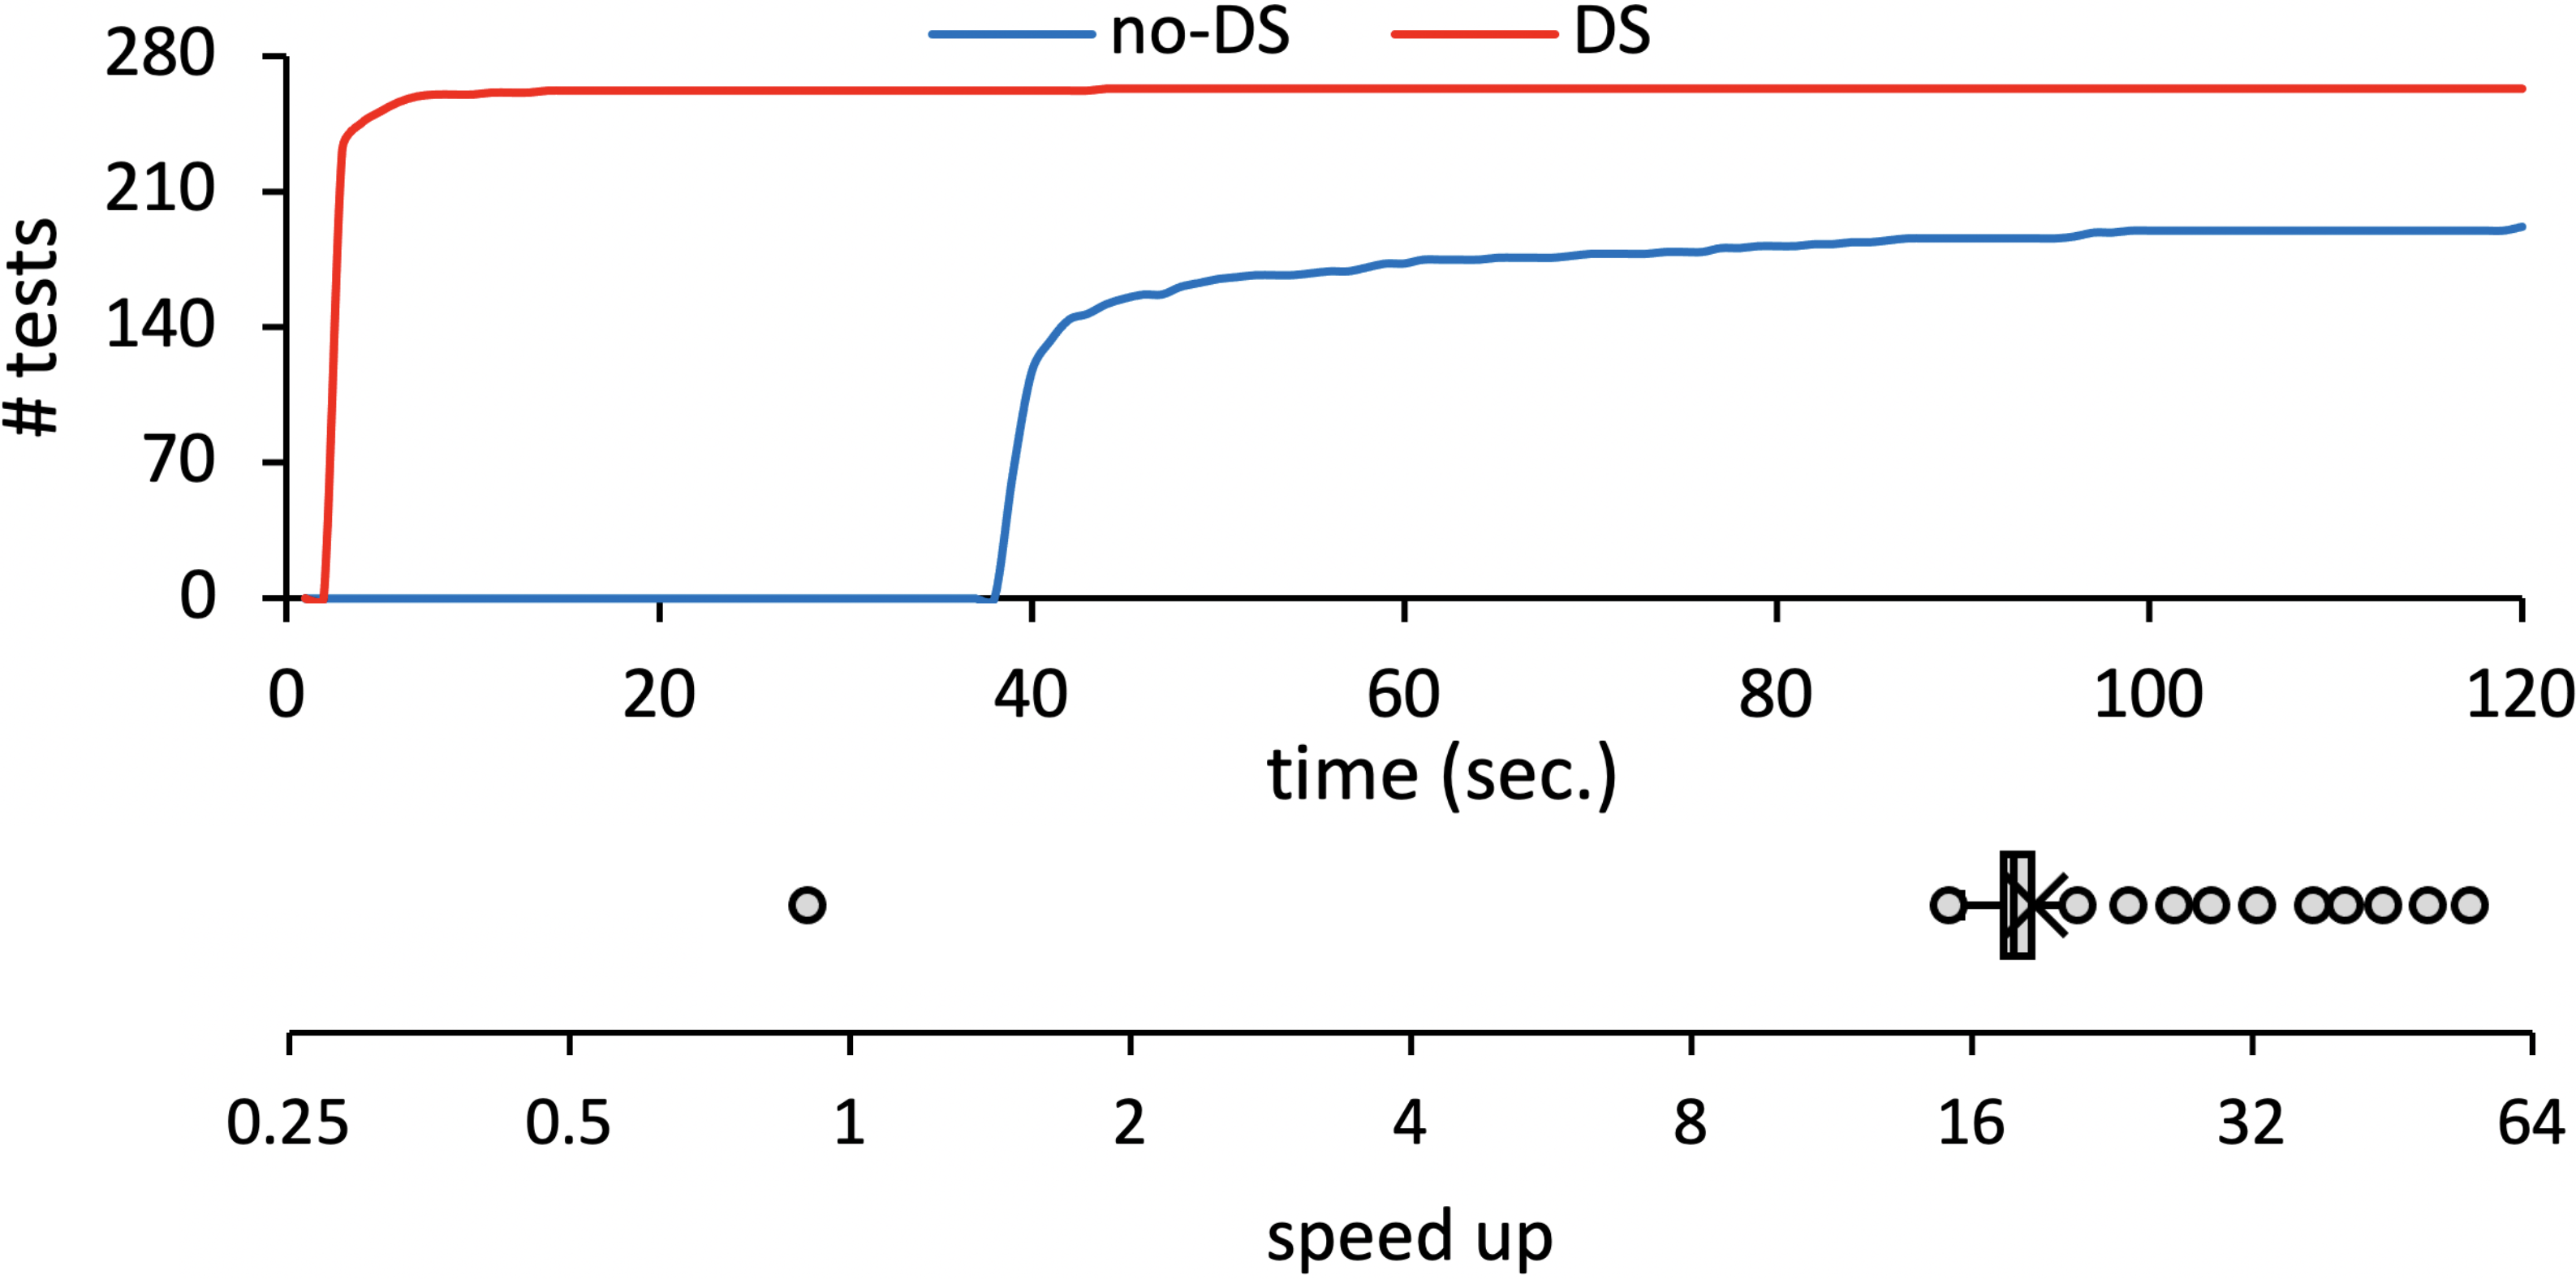
\includegraphics[width=\linewidth]{img/conc-analysis-time}
  \vspace*{-1.5em}
  \caption{Analysis time for Lodash 4 \textit{original} tests without (no-DS)
  and with (DS) dynamic shortcuts within 5 minutes}
  \label{fig:conc-analysis-time}
  \vspace*{-1.5em}
\end{figure}

\begin{figure}[t]
  \centering
  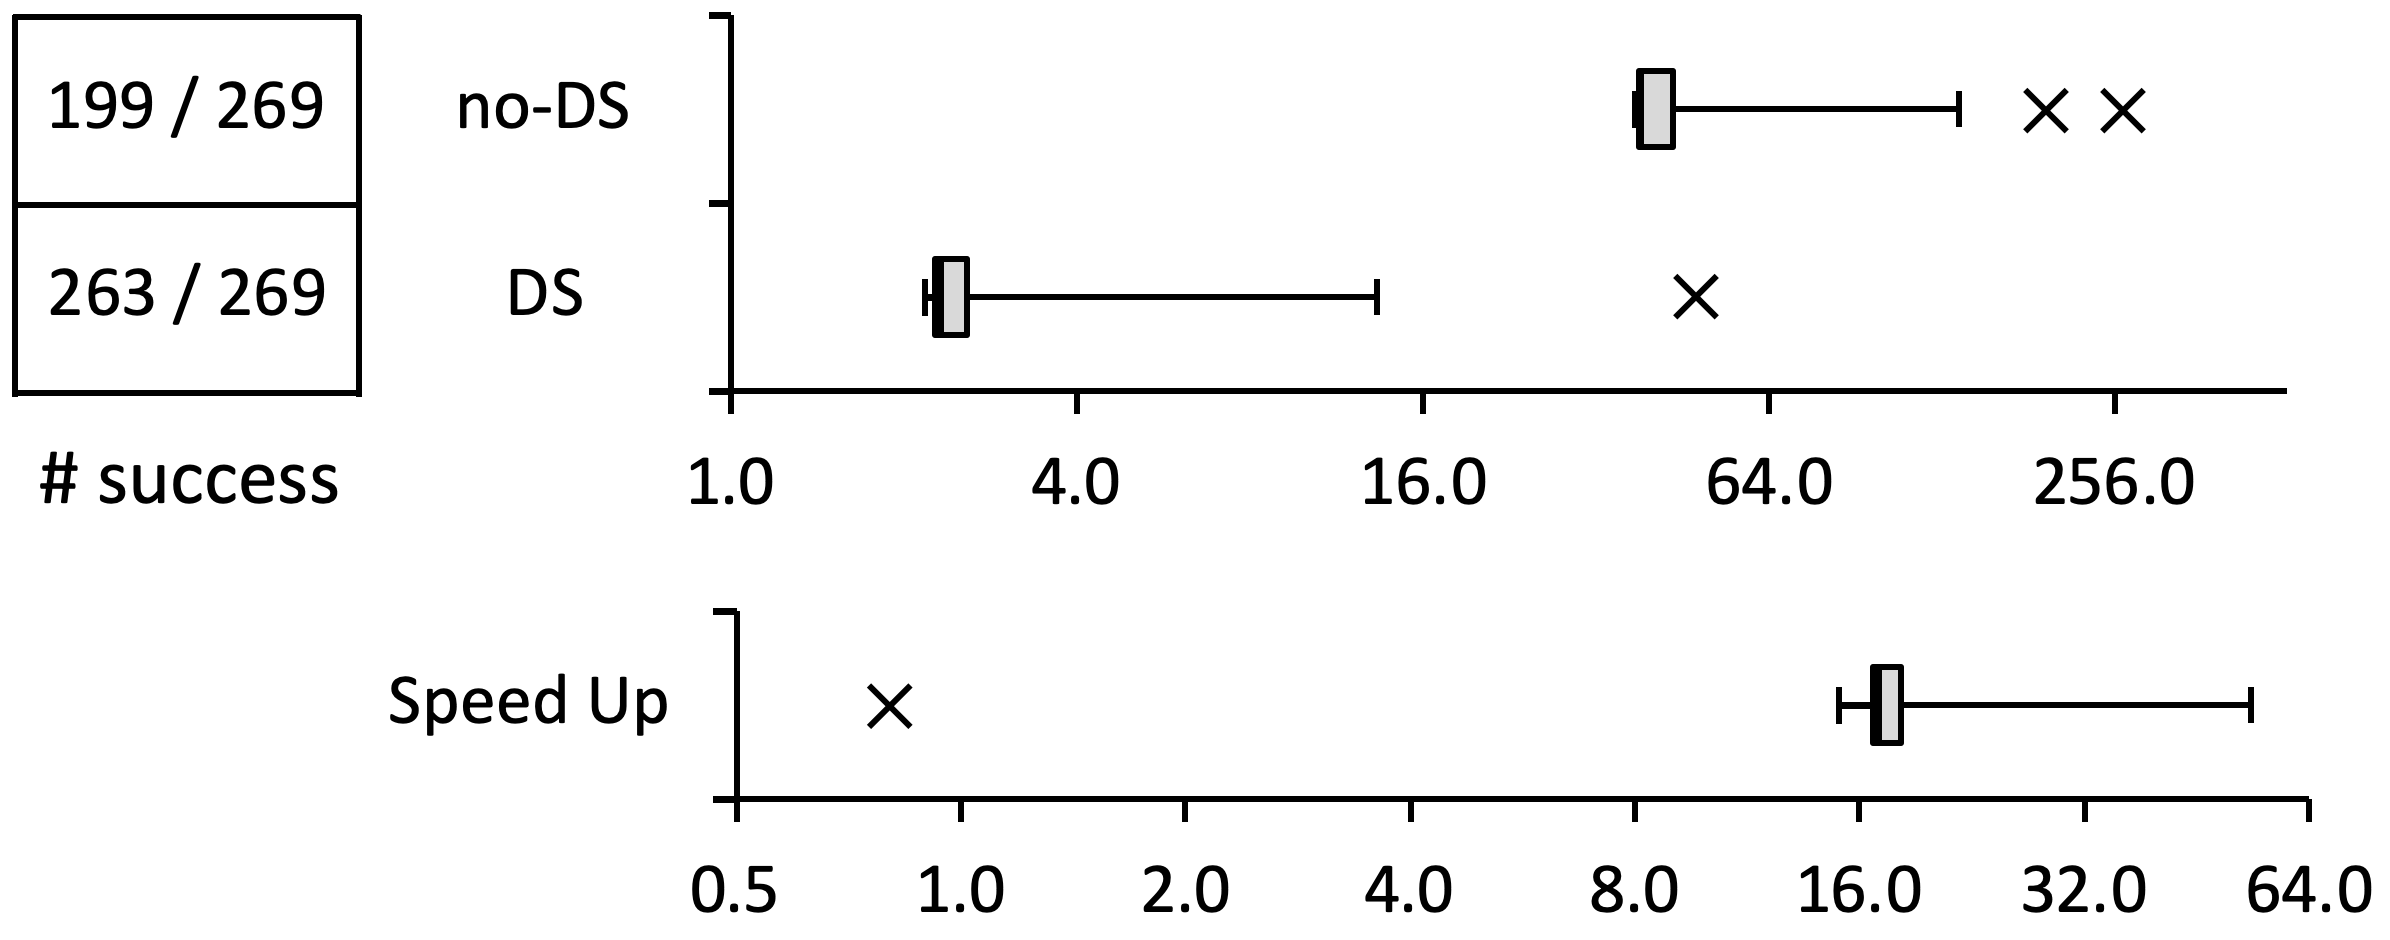
\includegraphics[width=\linewidth]{img/abs-analysis-time}
  \vspace*{-1.5em}
  \caption{Analysis time for Lodash 4 \textit{abstracted} tests without (no-DS)
  and with (DS) dynamic shortcuts within 5 minutes}
  \label{fig:abs-analysis-time}
  \vspace*{-1.5em}
\end{figure}

To evaluate the effectiveness of using dynamic shortcuts, we performed static
analysis of 269 Lodash 4 tests with and without dynamic shortcuts.
Figure~\ref{fig:conc-analysis-time} depicts cumulative distribution charts for
their analysis time and a box plot in a logarithmic scale for speed up after
applying dynamic shortcuts.  In the upper chart, the $x$-axis is time and the
$y$-axis shows the number of tests within the time.  While the baseline analysis
(no-DS) finished analysis of 200 out of 269 tests within 5 minutes, our tool
(DS) finished analysis of \inred{263} tests using dynamic shortcuts.  For finished
tests, the average analysis time is \inred{49.57} seconds for no-DS and \inred{2.78} seconds for
DS.  Among 200 tests analyzed by no-DS, \inred{two tests} are timeout in DS, thus
\inred{198} tests are analyzable by both analyzers. For them, we depict the box plot for
analysis speed up by dynamic shortcuts.  It shows that DS
outperforms no-DS up to \inred{54.98$\x$} and \inred{19.96$\x$} on
average.  Only for one test using $\jscode{_.sample}$, which
randomly samples a value from a given array, DS showed
\inred{0.90$\x$ speed of no-DS due to 24 times uses} of dynamic shortcuts.

Note that since most tests use concrete values instead of
non-deterministic inputs, they can be analyzed by a few number of dynamic shortcuts.
In fact, among 269 tests, \inred{262} tests are analyzed
by a single dynamic shortcut without using abstract semantics.
However, in real-world JavaScript programs, arguments of library
functions may include non-deterministic inputs.
To evaluate $\tool$ in a real-world setting,
we modified the tests to use abstract values.
We made abstract values by randomly selecting literals and replacing
one of them with its corresponding abstract value.
For example, if we select a numeric literal \jscode{42}, we modified it to the abstract numeric value
$\top_{\code{num}}$, which represents all the numeric values.
In the remaining section, we evaluated $\tool$ using the \textit{original} tests
and the \textit{abstracted} tests.

For abstracted tests as well, DS outperformed no-DS.
Figure~\ref{fig:abs-analysis-time} shows the analysis time of the abstracted tests.
Among 269 abstracted tests, no-DS finished analysis of 158 tests within 5 minutes,
but DS finished analysis of \inred{167} tests.  For finished tests, the average analysis
time is \inred{44.88} seconds for no-DS and \inred{42.28} seconds for DS. Among 158 tests analyzed by no-DS, DS
timed-out for \inred{15} tests.  For \inred{143} tests analyzable by both analyzers,
DS outperformed no-DS up to \inred{50.60$\x$} and \inred{6.30$\x$} on average.
\inred{Except for 6 test cases, using dynamic shortcut did show speed up.}

\begin{figure}[t]
  \centering
  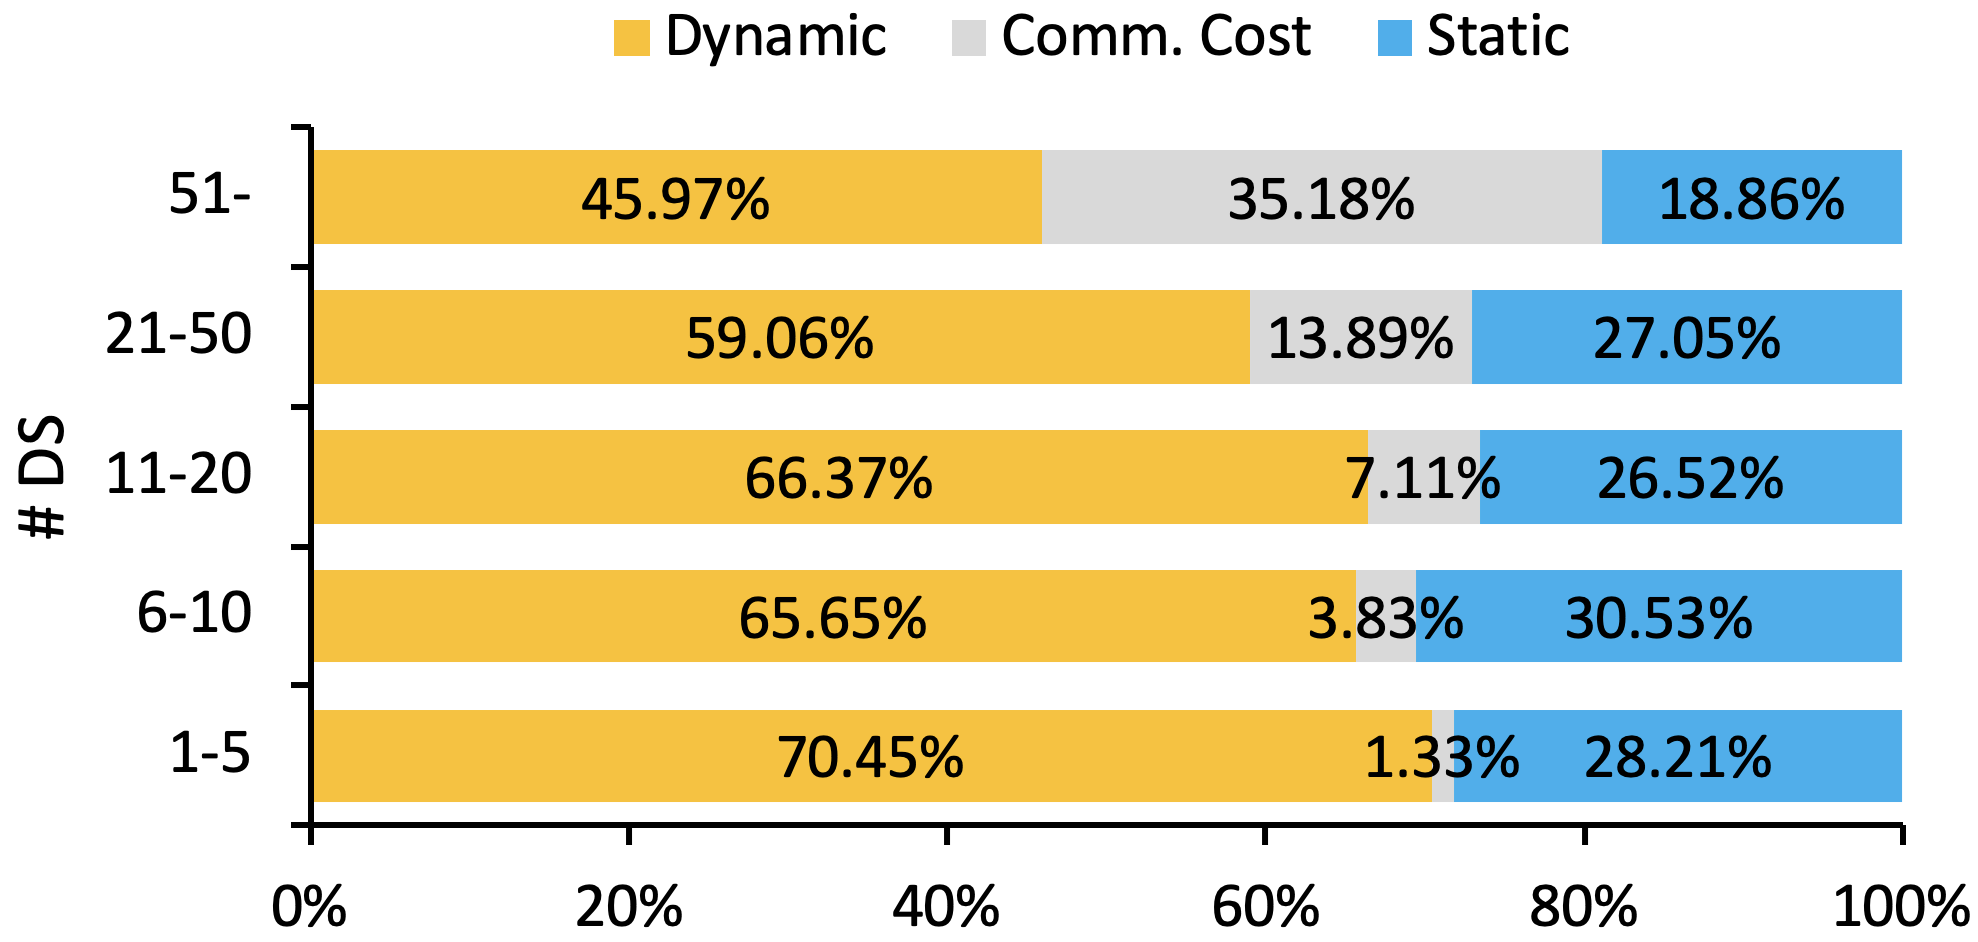
\includegraphics[width=\linewidth]{img/abs-analysis-ratio}
  \vspace*{-1.5em}
  \caption{Analysis time ratio for \inred{143} \textit{abstracted} tests}
  \label{fig:abs-analysis-ratio}
  \vspace*{-1.5em}
\end{figure}

\begin{table*}[t]
  \caption{Number of original (orig.) and abstracted (abs.) tests using dynamic shortcuts
only for each JavaScript built-in library}
  \label{table:func-replace}
  \vspace*{-1em}
  \centering
  \scriptsize
  \[
\quad
    \begin{array}{c|l|c|c?c|l|c|c?c|l|c|c}

      \myhead{Object}       {Function}        {\# Replaced}

      \mysutf{1}{}          {Array    }  {203 / 203}{ 90 / 116} & \mysutf{1}{}             {String     }  { 20 /  20}{  9 /  10} & \mysutf{1}{}       {Object        }  {263 / 263}{151 / 167} \mylinefff
      \mysutf{1}{}          {new Array}  {  0 /   0}{  0 /  10} & \mysutf{1}{}             {toString   }  {  0 /   0}{  0 /  33} & \mysutf{1}{}       {new Object    }  {  0 /   0}{  0 /   3} \mylinefff
      \mysutf{1}{}          {isArray  }  {263 / 263}{144 / 167} & \mysutf{1}{}             {valueOf    }  {  0 /   0}{  0 /  12} & \mysutf{1}{}       {getPrototypeOf}  { 56 /  56}{ 24 /  29} \mylinefff
      \mysutf{1}{}          {concat   }  {263 / 263}{163 / 167} & \mysutt{1}{}             {charAt     }  {  7 /   7}{  5 /   5} & \mysutf{1}{}       {create        }  {263 / 263}{164 / 167} \mylinefff
      \mysutf{1}{}          {join     }  {263 / 263}{166 / 167} & \mysutf{1}{}             {charCodeAt }  { 15 /  15}{  3 /   4} & \mysutf{1}{Object} {defineProperty}  {263 / 263}{160 / 167} \mylinefff
      \mysutf{1}{}          {pop      }  { 25 /  25}{  9 /  13} & \mysutt{1}{}             {indexOf    }  {  2 /   2}{  1 /   1} & \mysbtt{1}{}       {freeze        }  {  1 /   1}{  1 /   1} \mylinefff
      \mysutf{2}{Array}     {push     }  {263 / 263}{150 / 167} & \mysutf{1}{String}       {match      }  { 25 /  25}{ 11 /  13} & \mysutf{1}{}       {keys          }  {263 / 263}{161 / 167} \mylinefff
      \mysutt{1}{}          {reverse  }  { 10 /  10}{  3 /   3} & \mysutf{1}{}             {replace    }  { 55 /  55}{ 19 /  26} & \mysutf{1}{}       {toString      }  {263 / 263}{129 / 167} \mylinefff
      \mysutf{1}{}          {shift    }  {  2 /   2}{  0 /   1} & \mysutf{1}{}             {slice      }  {263 / 263}{165 / 167} & \mysutf{1}{}       {hasOwnProperty}  {263 / 263}{161 / 167} \mylinefft
      \mysutf{1}{}          {slice    }  {263 / 263}{164 / 167} & \mysutf{1}{}             {split      }  {  5 /   5}{  0 /   1} & \mysutf{1}{}       {parseInt}        {  1 /   1}{  0 /   1} \mylinefff
      \mysutf{1}{}          {sort     }  { 69 /  69}{ 26 /  28} & \mysutf{1}{}             {substring  }  {214 / 214}{ 91 / 121} & \mysutf{1}{Global} {isNaN   }        { 15 /  15}{  9 /  25} \mylinefff
      \mysutf{1}{}          {splice   }  { 25 /  25}{  6 /  11} & \mysutf{1}{}             {toLowerCase}  {214 / 214}{ 90 / 121} & \mysbtt{1}{}       {isFinite}        {  3 /   3}{  1 /   1} \mylinefft
      \mysutt{1}{}          {unshift  }  {  2 /   2}{  1 /   1} & \mysutf{1}{}             {toUpperCase}  { 10 /  10}{  4 /   6} & \mysbtt{1}{}       {RegExp    }      {263 / 263}{167 / 167} \mylineftf
      \mysutf{1}{}          {indexOf  }  { 94 /  94}{ 22 /  47} & \mysutt{2}{Boolean}      {Boolean}      {  3 /   3}{  2 /   2} & \mysutf{2}{RegExp} {new RegExp}      {  0 /   0}{  0 /   1} \mylinefff
      \mysutf{1}{}          {every    }  { 92 /  92}{ 23 /  32} & \mysutf{1}{}             {valueOf}      {  0 /   0}{  0 /   6} & \mysbtt{1}{}       {exec      }      {263 / 263}{167 / 167} \mylinettf
      \mysutt{1}{}          {ceil }      { 36 /  36}{  8 /   8} & \mysutf{2}{Number}       {Number }      {  2 /   2}{  1 /   2} & \mysutf{1}{}       {test      }      {263 / 263}{158 / 167} \mylinefft
      \mysuff{1}{}          {floor}      { 16 /  17}{  4 /   5} & \mysutf{1}{}             {valueOf}      {  0 /   0}{  0 /  16} & \mysutf{1}{}       {Error         }  {  1 /   1}{  0 /   1} \mylineftf
      \mysutf{1}{Math}      {max  }      {263 / 263}{134 / 167} & \mysutt{1}{}             {toString}     {263 / 263}{167 / 167} & \mysutf{2}{Error}  {new Error     }  {  0 /   0}{  0 /   8} \mylinefff
      \mysutf{1}{}          {min  }      { 64 /  64}{ 15 /  48} & \mnsutf{1}{Function}     {apply   }     {263 / 263}{124 / 167} & \mysutf{1}{}       {new RangeError}  {  0 /   0}{  0 /   3} \mylinefff
      \mysutt{1}{}          {pow  }      { 11 /  11}{  5 /   5} & \mysuff{1}{}             {call    }     {262 / 263}{ 50 / 167} & \mysutf{1}{}       {new TypeError }  {  0 /   0}{  0 /   9}
    \end{array}
  \]
  \vspace*{-1em}
\end{table*}

Unlike for the original tests, analysis of \inred{143} abstracted tests invoked
\inred{16.05} dynamic shortcuts.  Because taking a dynamic shortcut
requires conversion between abstract states and {\sealed} values
and their exchanges between the static analyzer and the dynamic analyzer,
using dynamic shortcuts multiple times may incur more performance
overhead than performance benefits by using {\sealed} execution.
One conjecture is that the communication cost between the static
analyzer and the dynamic analyzer may be proportional to the number of
dynamic shortcuts.

To experimentally evaluate the conjecture, we investigated the relationship between
the communication cost between analyzers and the number of dynamic shortcuts.
For \inred{198} original tests, the communication cost was only
\inred{3.51\%} compared to the analysis time of no-DS.  However, for \inred{143}
abstracted tests, the communication cost was \inred{82.49\%} compared to the analysis
time of no-DS.  Figure~\ref{fig:abs-analysis-ratio} presents the
analysis time ratio for \inred{143} abstracted tests.
The $x$-axis represents the time ratio normalized by the total analysis time of
no-DS and the $y$-axis denotes the number of dynamic
shortcuts and the number of corresponding tests.
For all \inred{143} tests, the communication cost (Comm. Cost) is larger than
both the static analysis time (Static) and the dynamic analysis
time (Dynamic).  When dynamic shortcuts are performed less than 10 times,
the communication cost is modest compared with the baseline static
analysis time.  However, the more dynamic shortcuts are performed,
the less the performance benefits by using dynamic shortcuts.
\inred{Specifically, when dynamic shortcuts are performed more than
20 times, Comm. Cost is even larger than no-DS.}
Based on this evaluation result, we believe that we can leverage
dynamic shortcuts by optimizing the communication cost between
the static analyzer and the dynamic analyzer.

\begin{figure}[t]
  \centering
  \begin{subfigure}[t]{0.48\textwidth}
    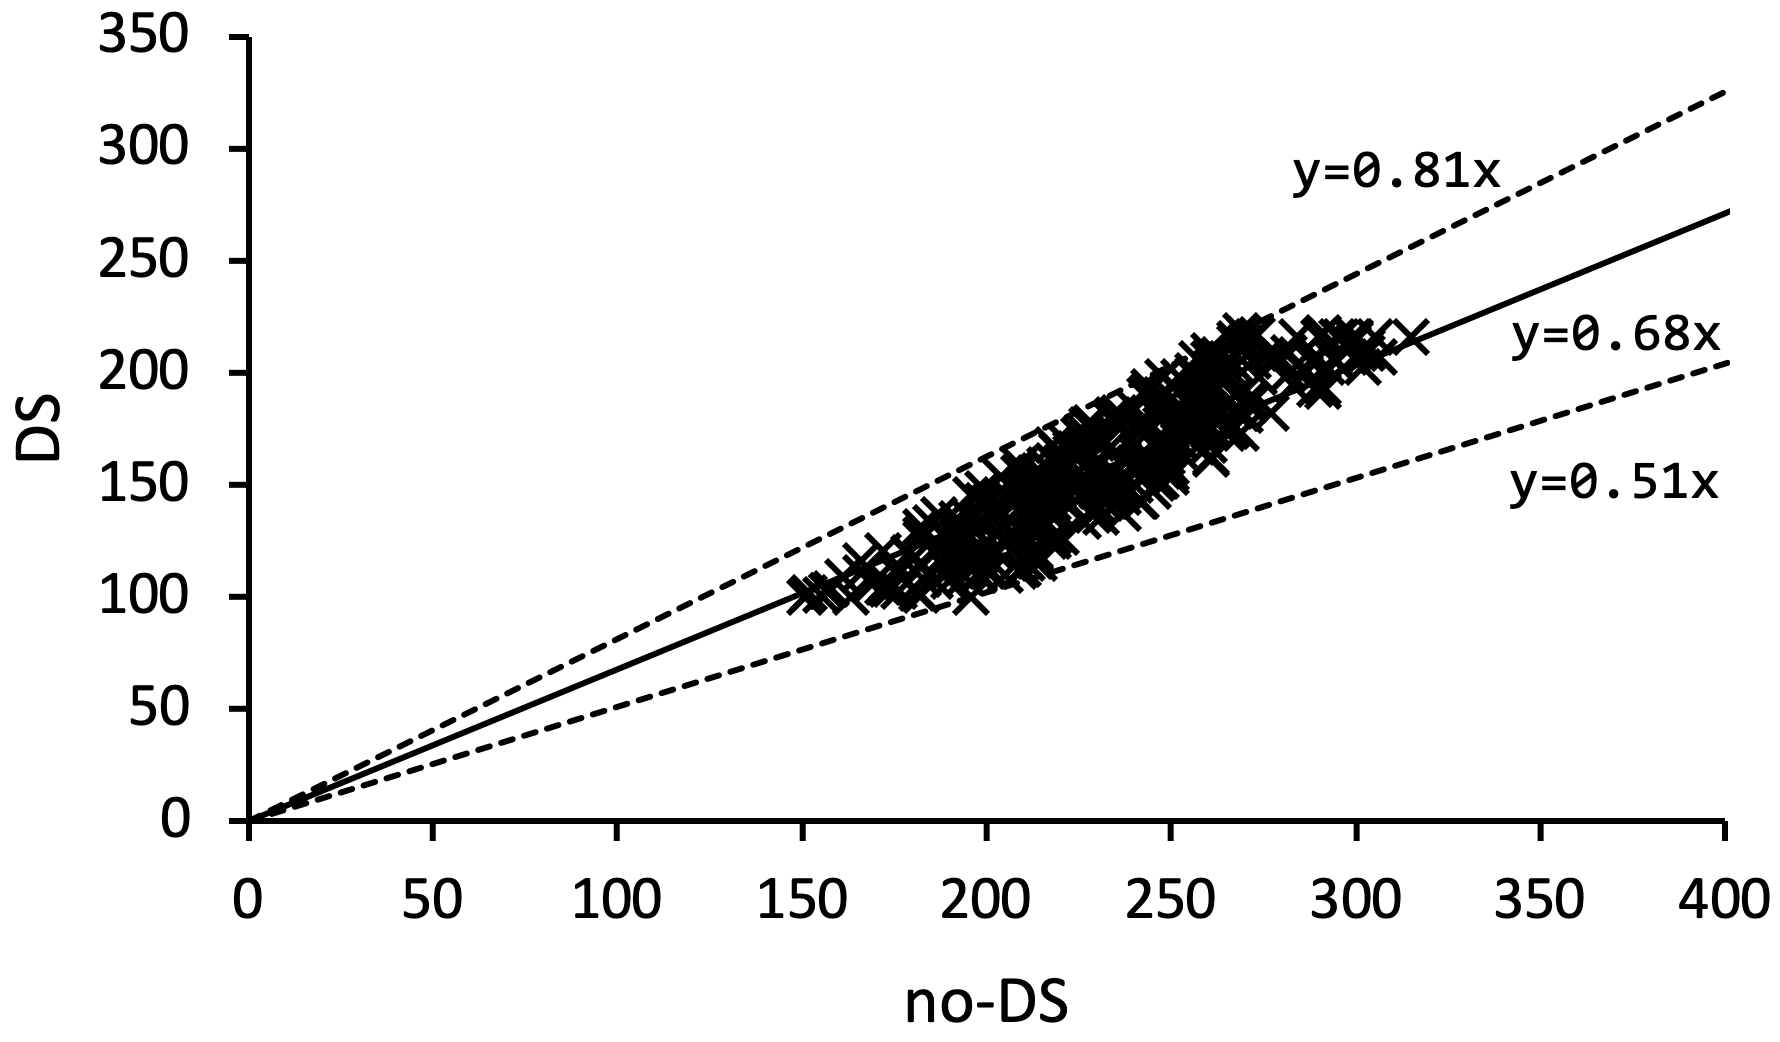
\includegraphics[width=\linewidth]{img/conc-precision}
    \vspace*{-1.5em}
    \caption{Reachable branches for \inred{198} \textit{original} tests}
    \label{fig:precision-fail}
  \end{subfigure}
  \begin{subfigure}[t]{0.48\textwidth}
    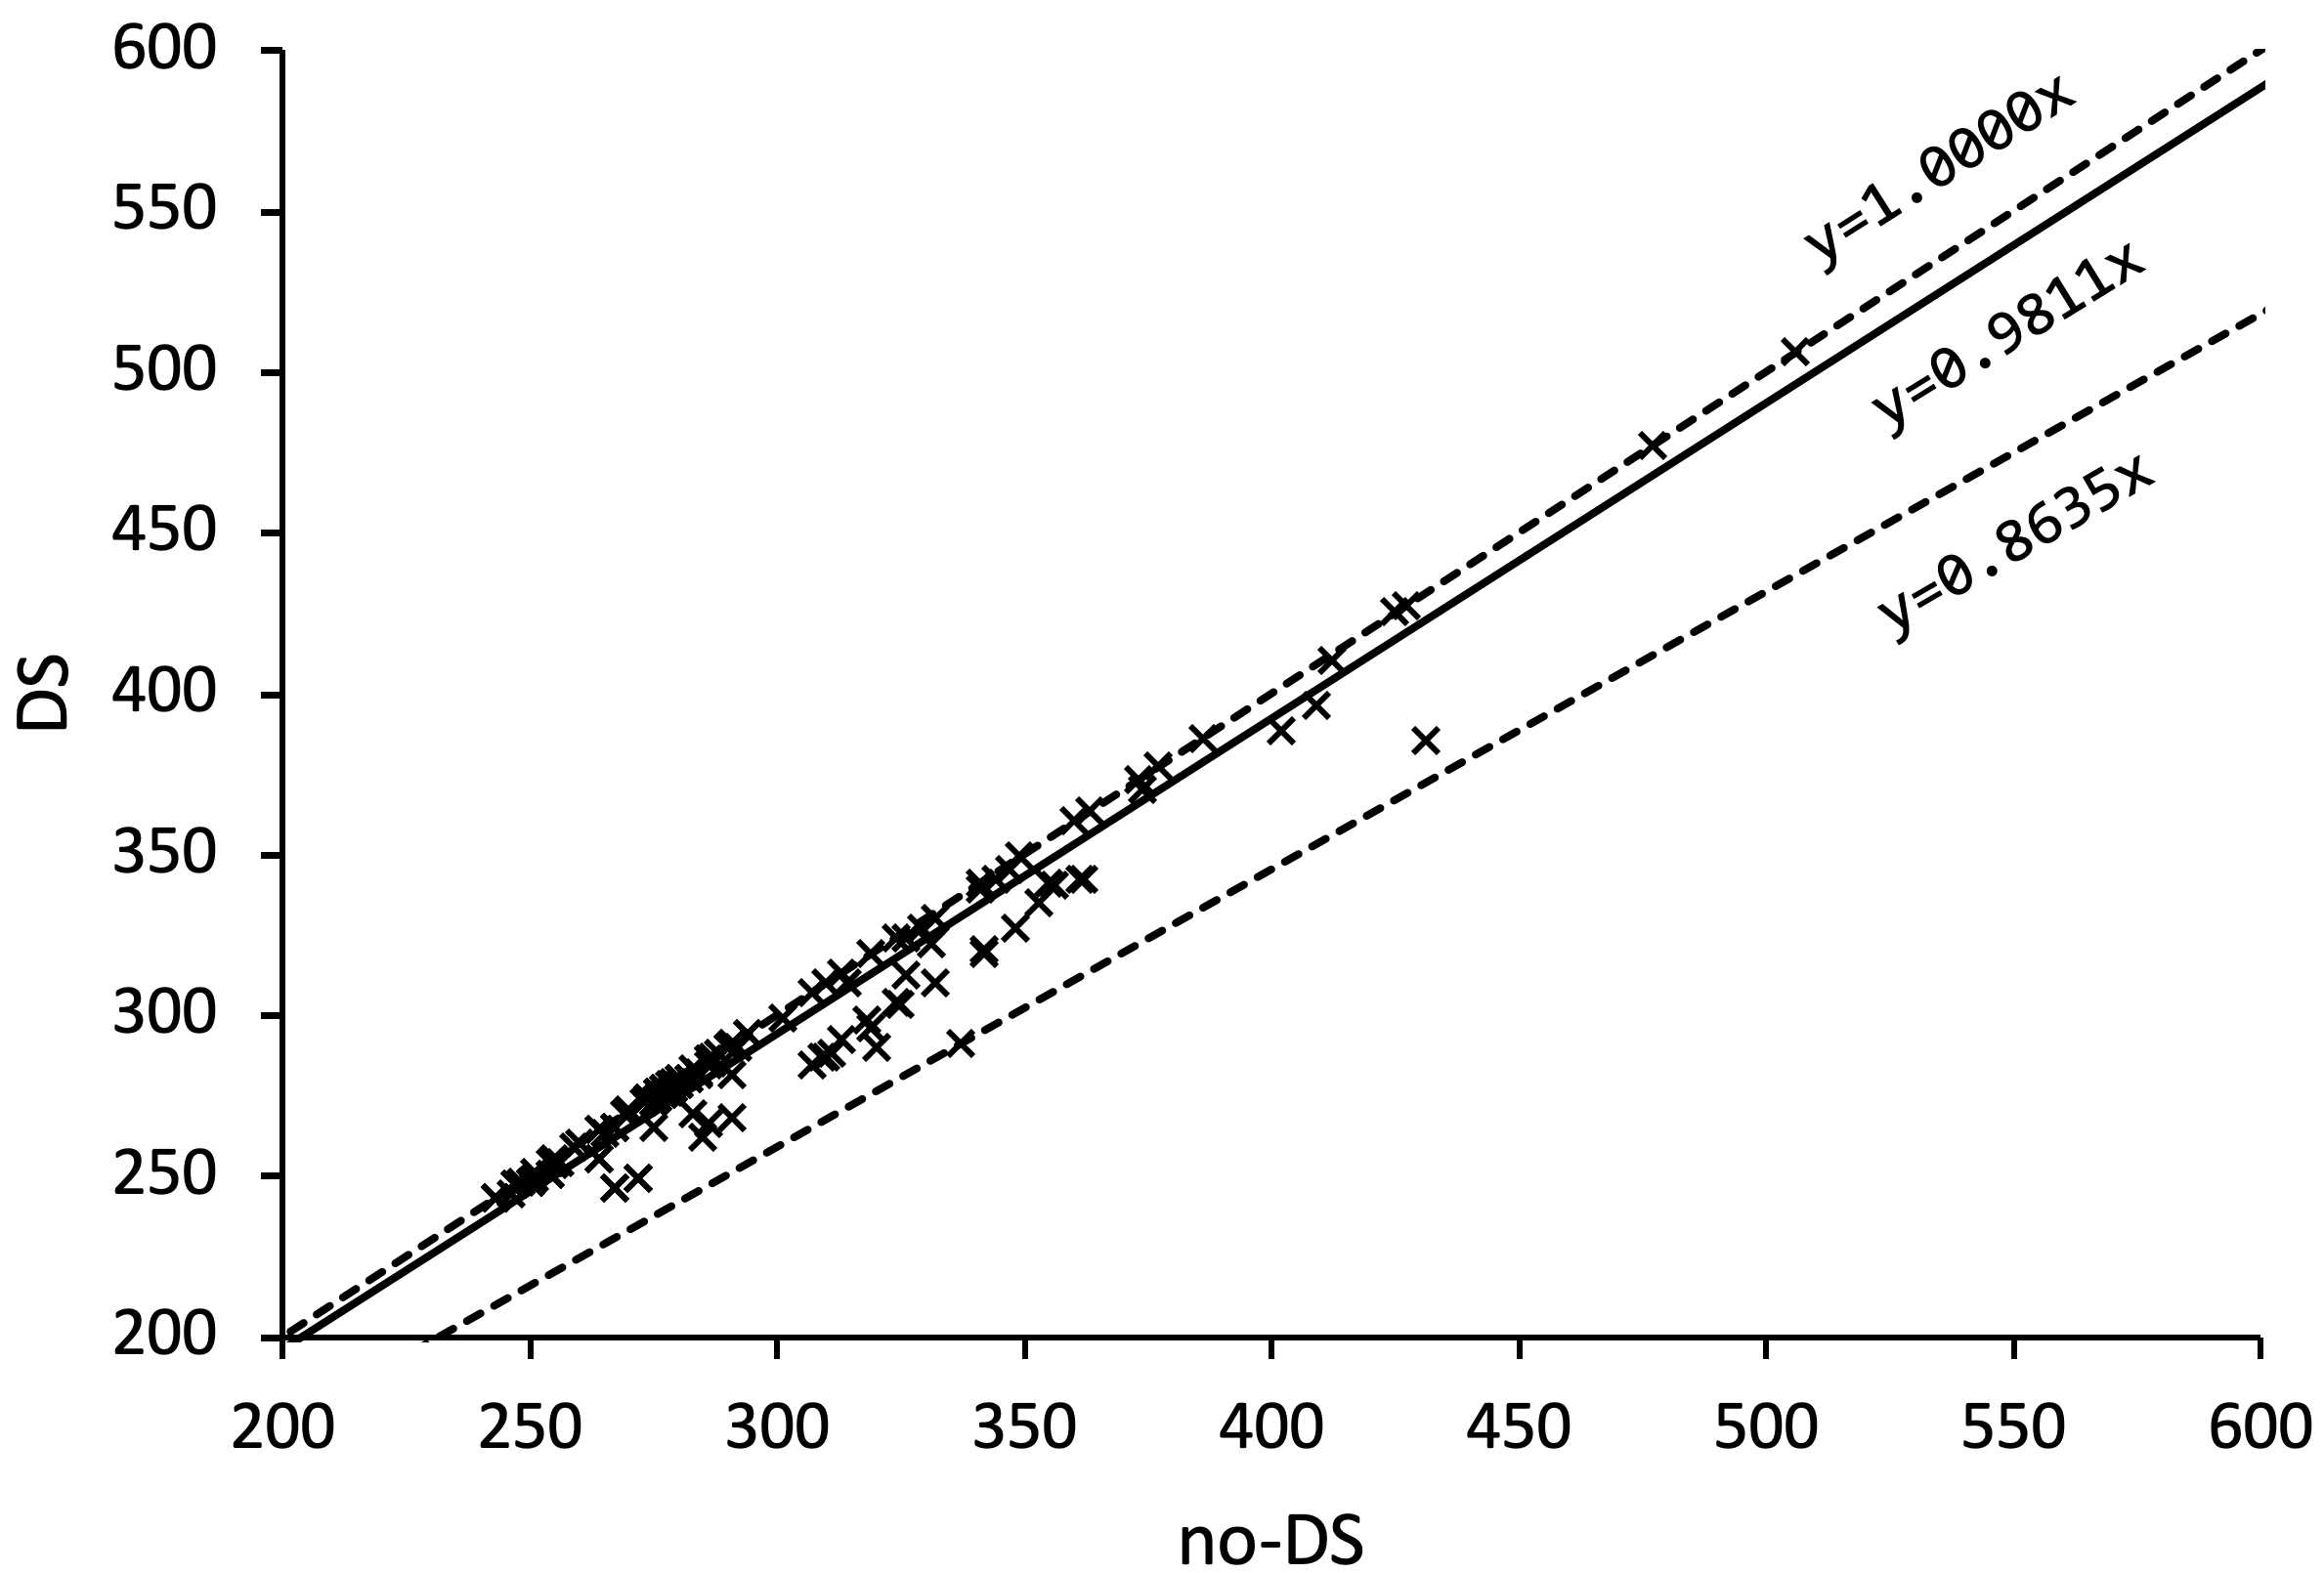
\includegraphics[width=\linewidth]{img/abs-precision}
    \vspace*{-1.5em}
    \caption{Reachable branches for \inred{143} \textit{abstracted} tests}
    \label{fig:precision-branch}
  \end{subfigure}
  \vspace*{-1em}
  \caption{Branch coverage of analysis without (no-DS) and with (DS) dynamic shortcuts}
  \label{fig:precision}
  \vspace*{-1.5em}
\end{figure}



\subsection{Precision Improvement}

To evaluate the analysis precision improvement of dynamic shortcuts,
we measured the number of \inred{assertion fails invoked by} no-DS and DS.
Because both no-DS and DS are sound,
high (low) \inred{number of assertion fails} denotes low (high) analysis precision.

Figure~\ref{fig:precision} depicts the comparison of the analysis
precision between no-DS and DS.  The $x$-axis and the $y$-axis denote
the number of \inred{assertion fails invoked} by no-DS and DS, respectively;
each \inred{circle} mark denotes each test \inred{in heatmap form. The darker the circle is, the more tests it indicates.} The top line
denotes the y=x line, and
the bottom solid line denotes the average improvement.
For \inred{198} original tests that are analyzable by both analyzers,
Figure~\ref{fig:precision}(a) shows that dynamic shortcuts
\inred{completely removed the assertion fails for 24 tests, reducing the nuber of assertion fails by 93\% on average.}
For \inred{143} abstracted tests that are analyzable by both analyzers,
Figure~\ref{fig:precision}(b) shows that dynamic shortcuts successfully cut down
the number of \inred{covered branches 12\% on average.}
Thus, on average, dynamic shortcuts removed analysis of \inred{93\%} and \inred{12\%} spurious alarms
for original and abstracted tests, respectively.

\section{Related Work}\label{sec:related}

Several researchers have introduced analysis technique to utilize dynamic
analysis for static analysis in three different ways: combined analysis,
automatic modeling, and pruning states.


\paragraph{Combined Analysis}

The most related previous work is the combined analysis that utilizes dynamic
analysis during Java static analysis introduced by \citet{concerto}.  They
proved that their combined analysis is sound and showed that it could
significantly improve the precision and performance of Java static analysis by
evaluating their tool, \concerto.  However, their approach have several
limitations compared to the dynamic shortcut.  First, they syntactically divides
a given program to \textit{applications} parts for static analysis and
\textit{frameworks} parts for dynamic analysis.  Thus, it is impossible to
freely switching between static and dynamic and even impossible to perform both
of static and dynamic analysis to the same program part in different contexts.
Besides, they introduced \textit{mostly-concrete interpretation} similar with
our sealed symbolic execution.  However, it supports only a special
\textit{unknown} value that represents any possible value.  Thus, it cannot
preserves the precision of complex abstract domains~\cite{safe, tajs, regex,
weaklySPE} frequently used in JavaScript static analysis.  In the other hand,
the sealed symbolic execution automatically detects whether the abstract
semantics for abstract values.  Finally, \concerto preserves the soundness when
the program satisfies the \textit{state separation hypothesis}.  They assume
that states of application and framework parts do not interrogated or
manipulated by each other.  While it is reasonable for static analysis of Java
applications using external libraries, the assumption is not satisfied for
JavaScript programs in general.  Unlike their approach, our approach does not
have any assumption between static and dynamic analysis parts.


\paragraph{Automatic Modeling}
For static analysis of JavaScript programs, modeling behaviors of built-in
libraries or host-dependent functions is required because they are opaque
codes.  Since manual modeling is error-prone, tedious, and labor-intensive,
several researchers~\cite{safewapi, safets} utilize type information to
automatically model their behaviors.  However, type information is too imprecise
to reflect the detailed semantics and is difficult to represent the
side-effects.  To alleviate the problem, \citet{mimic} introduced the technique
to infer JavaScript codes for opaque codes using concrete execution.  They
captured the effects of opaque codes on user objects by collecting partial
execution traces and synthesized JavaScript codes based on the extracted
behaviors.  They also leveraged ES6 \jscode{Proxy} objects to capture the
effects on user objects.  Instead of synthesizing JavaScript codes,
\citet{opaque-model} presented a \textit{Sample-Run-Abstract (SRA)} approach for
on-demand modeling thus they focused on the current abstract state during static
analysis.  It first \textit{samples} concrete states in a well-distributed way,
\textit{runs} each sampled state on a JavaScript engine, and \textit{abstract}
executions results.  However, all of previous works sacrifice the soundness of
static analysis.  On the other hand, while the dynamic shortcut is not
applicable for all invocation of opaque functions, it is sound if it is
applicable.


\paragraph{Pruning Analysis Scopes}
Another approach to utilize dynamic analysis for JavaScript static analysis is
to prune the scope of analysis.  \citet{blended} introduced \textit{blended
taint analysis} that specializes JavaScript dynamic language features such as
dynamic code generation (e.g. \jscode{eval}) or variadic function calls.  They
first performs dynamic analysis to collect traces with concrete values used in
dynamic language features and restrict the semantics of features based on the
collected traces during static analysis.  \citet{battles, eha} utilizes three
different points to reduce analysis scopes: initial states, dynamically loaded
files, and event handlers.  They dumped the initial states from a specific web
browser to focus on analyzing the behaviors of web browsers running on the
browser.  Then, they collected paths of dynamically loaded files via concrete
executions and utilized the path information in static analysis.  For event
handlers, they intentionally analyzed partial execution flows using concrete
user events.  They collected concrete states for each entry of event handler
during dynamic analysis, merged them to a single abstract state, and analyzed
the event handler with the abstract state.  Unfortunately, all of them does not
preserve soundness of static analysis unlike the dynamic shortcut.


% \subsection{Abstract Counting}
% 
% \begin{itemize}
%   \item Improving flow analyses via $\Gamma$CFA: Abstract garbage collection and
%     counting~\cite{abstract-gc-counting}
%   \item Revisiting recency abstraction for JavaScript: towards an intuitive,
%     compositional, and efficient heap abstraction~\cite{revisit-recency}
% \end{itemize}

% \subsection{Access Analysis}
% 
% \begin{itemize}
%   \item Access Analysis-Based Tight Localization of Abstract
%     Memories~\cite{func-local}
%   \item Design and implementation of sparse global analyses for C-like
%     languages~\cite{sparse}
% \end{itemize}

\section{Conclusion}\label{sec:conclusion}
We presented a novel technique for JavaScript static analysis using \textit{dynamic shortcuts}.
It can significantly accelerate static
analysis by freely leveraging high performance of dynamic analysis for
concretely executable program parts.  To maximize such benefits,
we proposed \textit{sealed symbolic execution}, which performs
concrete execution using sealed symbolic values for abstract values.
We formally defined static analysis using dynamic shortcuts in the
abstract interpretation framework and proved its soundness and termination.
We developed $\tool$ as a prototype implementation of the proposed approach
by extending a combination of the state-of-the-art static and dynamic
analyzers SAFE and Jalangi.  Our tool accelerates the speed
of static analysis \inred{19.96}x for original tests and \inred{6.30}x for
abstracted tests of Lodash 4 library.  Moreover, it detects \inred{6} more
dead branches by using sealed symbolic execution instead of
manual modeling for \inred{12} opaque functions on average.


\bibliographystyle{ACM-Reference-Format}
\bibliography{ref}

\end{document}
\endinput
